\documentclass[a4paper]{book}
\usepackage{a4wide}
\usepackage{makeidx}
\usepackage{graphicx}
\usepackage{multicol}
\usepackage{float}
\usepackage{listings}
\usepackage{color}
\usepackage{textcomp}
\usepackage{alltt}
\usepackage{times}
\usepackage{ifpdf}
\ifpdf
\usepackage[pdftex,
            pagebackref=true,
            colorlinks=true,
            linkcolor=blue,
            unicode
           ]{hyperref}
\else
\usepackage[ps2pdf,
            pagebackref=true,
            colorlinks=true,
            linkcolor=blue,
            unicode
           ]{hyperref}
\usepackage{pspicture}
\fi
\usepackage[utf8]{inputenc}
\usepackage{doxygen}
\lstset{language=C++,inputencoding=utf8,basicstyle=\footnotesize,breaklines=true,breakatwhitespace=true,tabsize=8,numbers=left }
\makeindex
\setcounter{tocdepth}{3}
\renewcommand{\footrulewidth}{0.4pt}
\begin{document}
\hypersetup{pageanchor=false}
\begin{titlepage}
\vspace*{7cm}
\begin{center}
{\Large Reference Manual}\\
\vspace*{1cm}
{\large Generated by Doxygen 1.6.1}\\
\vspace*{0.5cm}
{\small Tue Feb 9 15:58:46 2016}\\
\end{center}
\end{titlepage}
\clearemptydoublepage
\pagenumbering{roman}
\tableofcontents
\clearemptydoublepage
\pagenumbering{arabic}
\hypersetup{pageanchor=true}
\chapter{Namespace Index}
\section{Namespace List}
Here is a list of all documented namespaces with brief descriptions:\begin{DoxyCompactList}
\item\contentsline{section}{\hyperlink{namespaceGeneratePDERestabFile}{GeneratePDERestabFile} (Generates a restab file for PDE )}{\pageref{namespaceGeneratePDERestabFile}}{}
\item\contentsline{section}{\hyperlink{namespaceGeochemistryRHSUtils}{GeochemistryRHSUtils} (Functions to use inside the method evalF for the Geochemistry RHS )}{\pageref{namespaceGeochemistryRHSUtils}}{}
\item\contentsline{section}{\hyperlink{namespaceTimings}{Timings} (An example of use of the C++11 chrono library )}{\pageref{namespaceTimings}}{}
\item\contentsline{section}{\hyperlink{namespaceUtils}{Utils} (Standard Types )}{\pageref{namespaceUtils}}{}
\end{DoxyCompactList}

\chapter{Class Index}
\section{Class Hierarchy}
This inheritance list is sorted roughly, but not completely, alphabetically:\begin{DoxyCompactList}
\item \contentsline{section}{Restab::Array$<$ T $>$}{\pageref{classRestab_1_1Array}}{}
\item \contentsline{section}{BESolverInput}{\pageref{classBESolverInput}}{}
\item \contentsline{section}{BESolverOutput}{\pageref{classBESolverOutput}}{}
\item \contentsline{section}{ChemicalPhase}{\pageref{classChemicalPhase}}{}
\item \contentsline{section}{ChemicalReaction}{\pageref{classChemicalReaction}}{}
\item \contentsline{section}{ChemicalSourceRate}{\pageref{classChemicalSourceRate}}{}
\item \contentsline{section}{ChemicalSpecies}{\pageref{classChemicalSpecies}}{}
\item \contentsline{section}{ChemicalSystem}{\pageref{classChemicalSystem}}{}
\item \contentsline{section}{ChemicalSystemState}{\pageref{classChemicalSystemState}}{}
\item \contentsline{section}{Timings::Chrono}{\pageref{classTimings_1_1Chrono}}{}
\item \contentsline{section}{CubicHermiteInterpolationInputSolver}{\pageref{classCubicHermiteInterpolationInputSolver}}{}
\item \contentsline{section}{CubicHermiteInterpolationOutputSolver}{\pageref{classCubicHermiteInterpolationOutputSolver}}{}
\item \contentsline{section}{CubicHermiteInterpolationSolver}{\pageref{classCubicHermiteInterpolationSolver}}{}
\item \contentsline{section}{Restab::DataCube}{\pageref{classRestab_1_1DataCube}}{}
\item \contentsline{section}{FESolverInput}{\pageref{classFESolverInput}}{}
\item \contentsline{section}{FESolverOutput}{\pageref{classFESolverOutput}}{}
\item \contentsline{section}{TraceOut::Flux}{\pageref{classTraceOut_1_1Flux}}{}
\item \contentsline{section}{GeochemistryParameters}{\pageref{classGeochemistryParameters}}{}
\item \contentsline{section}{GetPot}{\pageref{classGetPot}}{}
\item \contentsline{section}{IBCFunction}{\pageref{classIBCFunction}}{}
\begin{DoxyCompactList}
\item \contentsline{section}{ConstantBCFunction}{\pageref{classConstantBCFunction}}{}
\end{DoxyCompactList}
\item \contentsline{section}{IFluxFunction}{\pageref{classIFluxFunction}}{}
\begin{DoxyCompactList}
\item \contentsline{section}{BurgersFluxFunction}{\pageref{classBurgersFluxFunction}}{}
\item \contentsline{section}{LinearFluxFunction}{\pageref{classLinearFluxFunction}}{}
\end{DoxyCompactList}
\item \contentsline{section}{IMasterSolver}{\pageref{classIMasterSolver}}{}
\begin{DoxyCompactList}
\item \contentsline{section}{MultiRateTRBDF2Solver}{\pageref{classMultiRateTRBDF2Solver}}{}
\item \contentsline{section}{SingleRateBESolver}{\pageref{classSingleRateBESolver}}{}
\item \contentsline{section}{SingleRateFESolver}{\pageref{classSingleRateFESolver}}{}
\item \contentsline{section}{SingleRateTRBDF2Solver}{\pageref{classSingleRateTRBDF2Solver}}{}
\end{DoxyCompactList}
\item \contentsline{section}{Restab::IndexDescription}{\pageref{classRestab_1_1IndexDescription}}{}
\item \contentsline{section}{INewtonFunction}{\pageref{classINewtonFunction}}{}
\begin{DoxyCompactList}
\item \contentsline{section}{BESolverNewtonFunction}{\pageref{classBESolverNewtonFunction}}{}
\item \contentsline{section}{TRBDF2SolverNewtonFunction}{\pageref{classTRBDF2SolverNewtonFunction}}{}
\end{DoxyCompactList}
\item \contentsline{section}{INewtonSolver}{\pageref{classINewtonSolver}}{}
\begin{DoxyCompactList}
\item \contentsline{section}{BasicNewtonSolver}{\pageref{classBasicNewtonSolver}}{}
\item \contentsline{section}{FixedJacobianNewtonSolver}{\pageref{classFixedJacobianNewtonSolver}}{}
\end{DoxyCompactList}
\item \contentsline{section}{IRHSFunction}{\pageref{classIRHSFunction}}{}
\begin{DoxyCompactList}
\item \contentsline{section}{AllenCahnRHSFunction}{\pageref{classAllenCahnRHSFunction}}{}
\item \contentsline{section}{GeochemistryRHSFunction}{\pageref{classGeochemistryRHSFunction}}{}
\item \contentsline{section}{HyperbolicEquationRusanovFlux}{\pageref{classHyperbolicEquationRusanovFlux}}{}
\end{DoxyCompactList}
\item \contentsline{section}{ISolverData}{\pageref{classISolverData}}{}
\begin{DoxyCompactList}
\item \contentsline{section}{MultiRateTRBDF2SolverData}{\pageref{classMultiRateTRBDF2SolverData}}{}
\item \contentsline{section}{SingleRateBESolverData}{\pageref{classSingleRateBESolverData}}{}
\item \contentsline{section}{SingleRateFESolverData}{\pageref{classSingleRateFESolverData}}{}
\item \contentsline{section}{SingleRateTRBDF2SolverData}{\pageref{classSingleRateTRBDF2SolverData}}{}
\end{DoxyCompactList}
\item \contentsline{section}{MasterSolution}{\pageref{classMasterSolution}}{}
\item \contentsline{section}{NulStreambuf}{\pageref{classNulStreambuf}}{}
\begin{DoxyCompactList}
\item \contentsline{section}{NulOStream}{\pageref{classNulOStream}}{}
\end{DoxyCompactList}
\item \contentsline{section}{TraceMng}{\pageref{classTraceMng}}{}
\begin{DoxyCompactList}
\item \contentsline{section}{BasicNewtonSolver}{\pageref{classBasicNewtonSolver}}{}
\item \contentsline{section}{BESolver}{\pageref{classBESolver}}{}
\item \contentsline{section}{BESolverUtils}{\pageref{classBESolverUtils}}{}
\item \contentsline{section}{FESolver}{\pageref{classFESolver}}{}
\item \contentsline{section}{FESolverUtils}{\pageref{classFESolverUtils}}{}
\item \contentsline{section}{FixedJacobianNewtonSolver}{\pageref{classFixedJacobianNewtonSolver}}{}
\item \contentsline{section}{MultiRateTRBDF2Solver}{\pageref{classMultiRateTRBDF2Solver}}{}
\item \contentsline{section}{SingleRateBESolver}{\pageref{classSingleRateBESolver}}{}
\item \contentsline{section}{SingleRateFESolver}{\pageref{classSingleRateFESolver}}{}
\item \contentsline{section}{SingleRateTRBDF2Solver}{\pageref{classSingleRateTRBDF2Solver}}{}
\end{DoxyCompactList}
\item \contentsline{section}{TraceOut}{\pageref{classTraceOut}}{}
\item \contentsline{section}{TRBDF2Solver}{\pageref{classTRBDF2Solver}}{}
\item \contentsline{section}{TRBDF2SolverInput}{\pageref{classTRBDF2SolverInput}}{}
\item \contentsline{section}{TRBDF2SolverOutput}{\pageref{classTRBDF2SolverOutput}}{}
\item \contentsline{section}{TRBDF2SolverParameters}{\pageref{classTRBDF2SolverParameters}}{}
\item \contentsline{section}{Restab::VariableDescription}{\pageref{classRestab_1_1VariableDescription}}{}
\item \contentsline{section}{vector}{\pageref{classstd_1_1vector}}{}
\end{DoxyCompactList}

\chapter{Class Index}
\section{Class List}
Here are the classes, structs, unions and interfaces with brief descriptions:\begin{DoxyCompactList}
\item\contentsline{section}{\hyperlink{classAllenCahnRHSFunction}{AllenCahnRHSFunction} }{\pageref{classAllenCahnRHSFunction}}{}
\item\contentsline{section}{\hyperlink{classRestab_1_1Array}{Restab::Array$<$ T $>$} }{\pageref{classRestab_1_1Array}}{}
\item\contentsline{section}{\hyperlink{classBasicNewtonSolver}{BasicNewtonSolver} }{\pageref{classBasicNewtonSolver}}{}
\item\contentsline{section}{\hyperlink{classBESolver}{BESolver} }{\pageref{classBESolver}}{}
\item\contentsline{section}{\hyperlink{classBESolverInput}{BESolverInput} }{\pageref{classBESolverInput}}{}
\item\contentsline{section}{\hyperlink{classBESolverNewtonFunction}{BESolverNewtonFunction} (Newton Function for BE Solver )}{\pageref{classBESolverNewtonFunction}}{}
\item\contentsline{section}{\hyperlink{classBESolverOutput}{BESolverOutput} (Output for the time step solver )}{\pageref{classBESolverOutput}}{}
\item\contentsline{section}{\hyperlink{classBESolverUtils}{BESolverUtils} }{\pageref{classBESolverUtils}}{}
\item\contentsline{section}{\hyperlink{classBurgersFluxFunction}{BurgersFluxFunction} }{\pageref{classBurgersFluxFunction}}{}
\item\contentsline{section}{\hyperlink{classChemicalPhase}{ChemicalPhase} }{\pageref{classChemicalPhase}}{}
\item\contentsline{section}{\hyperlink{classChemicalReaction}{ChemicalReaction} }{\pageref{classChemicalReaction}}{}
\item\contentsline{section}{\hyperlink{classChemicalSourceRate}{ChemicalSourceRate} }{\pageref{classChemicalSourceRate}}{}
\item\contentsline{section}{\hyperlink{classChemicalSpecies}{ChemicalSpecies} }{\pageref{classChemicalSpecies}}{}
\item\contentsline{section}{\hyperlink{classChemicalSystem}{ChemicalSystem} }{\pageref{classChemicalSystem}}{}
\item\contentsline{section}{\hyperlink{classChemicalSystemState}{ChemicalSystemState} }{\pageref{classChemicalSystemState}}{}
\item\contentsline{section}{\hyperlink{classTimings_1_1Chrono}{Timings::Chrono} }{\pageref{classTimings_1_1Chrono}}{}
\item\contentsline{section}{\hyperlink{classConstantBCFunction}{ConstantBCFunction} (Class to store the Dirichlet boundary condition for the Hyperbolic PDE )}{\pageref{classConstantBCFunction}}{}
\item\contentsline{section}{\hyperlink{classCubicHermiteInterpolationInputSolver}{CubicHermiteInterpolationInputSolver} }{\pageref{classCubicHermiteInterpolationInputSolver}}{}
\item\contentsline{section}{\hyperlink{classCubicHermiteInterpolationOutputSolver}{CubicHermiteInterpolationOutputSolver} }{\pageref{classCubicHermiteInterpolationOutputSolver}}{}
\item\contentsline{section}{\hyperlink{classCubicHermiteInterpolationSolver}{CubicHermiteInterpolationSolver} (Interpolator for the components that are not active )}{\pageref{classCubicHermiteInterpolationSolver}}{}
\item\contentsline{section}{\hyperlink{classRestab_1_1DataCube}{Restab::DataCube} }{\pageref{classRestab_1_1DataCube}}{}
\item\contentsline{section}{\hyperlink{classFESolver}{FESolver} }{\pageref{classFESolver}}{}
\item\contentsline{section}{\hyperlink{classFESolverInput}{FESolverInput} }{\pageref{classFESolverInput}}{}
\item\contentsline{section}{\hyperlink{classFESolverOutput}{FESolverOutput} }{\pageref{classFESolverOutput}}{}
\item\contentsline{section}{\hyperlink{classFESolverUtils}{FESolverUtils} }{\pageref{classFESolverUtils}}{}
\item\contentsline{section}{\hyperlink{classFixedJacobianNewtonSolver}{FixedJacobianNewtonSolver} }{\pageref{classFixedJacobianNewtonSolver}}{}
\item\contentsline{section}{\hyperlink{classTraceOut_1_1Flux}{TraceOut::Flux} }{\pageref{classTraceOut_1_1Flux}}{}
\item\contentsline{section}{\hyperlink{classGeochemistryParameters}{GeochemistryParameters} (Parameters necessary to build the Geochemistry RHS Function )}{\pageref{classGeochemistryParameters}}{}
\item\contentsline{section}{\hyperlink{classGeochemistryRHSFunction}{GeochemistryRHSFunction} (Geochemistry function )}{\pageref{classGeochemistryRHSFunction}}{}
\item\contentsline{section}{\hyperlink{classGetPot}{GetPot} }{\pageref{classGetPot}}{}
\item\contentsline{section}{\hyperlink{classHyperbolicEquationRusanovFlux}{HyperbolicEquationRusanovFlux} }{\pageref{classHyperbolicEquationRusanovFlux}}{}
\item\contentsline{section}{\hyperlink{classIBCFunction}{IBCFunction} }{\pageref{classIBCFunction}}{}
\item\contentsline{section}{\hyperlink{classIFluxFunction}{IFluxFunction} }{\pageref{classIFluxFunction}}{}
\item\contentsline{section}{\hyperlink{classIMasterSolver}{IMasterSolver} }{\pageref{classIMasterSolver}}{}
\item\contentsline{section}{\hyperlink{classRestab_1_1IndexDescription}{Restab::IndexDescription} }{\pageref{classRestab_1_1IndexDescription}}{}
\item\contentsline{section}{\hyperlink{classINewtonFunction}{INewtonFunction} }{\pageref{classINewtonFunction}}{}
\item\contentsline{section}{\hyperlink{classINewtonSolver}{INewtonSolver} }{\pageref{classINewtonSolver}}{}
\item\contentsline{section}{\hyperlink{classIRHSFunction}{IRHSFunction} }{\pageref{classIRHSFunction}}{}
\item\contentsline{section}{\hyperlink{classISolverData}{ISolverData} }{\pageref{classISolverData}}{}
\item\contentsline{section}{\hyperlink{classLinearFluxFunction}{LinearFluxFunction} (Linear flux for the Hyperbolic PDE )}{\pageref{classLinearFluxFunction}}{}
\item\contentsline{section}{\hyperlink{classMasterSolution}{MasterSolution} (Class useful to store only some information from the SolverData class )}{\pageref{classMasterSolution}}{}
\item\contentsline{section}{\hyperlink{classMultiRateTRBDF2Solver}{MultiRateTRBDF2Solver} }{\pageref{classMultiRateTRBDF2Solver}}{}
\item\contentsline{section}{\hyperlink{classMultiRateTRBDF2SolverData}{MultiRateTRBDF2SolverData} }{\pageref{classMultiRateTRBDF2SolverData}}{}
\item\contentsline{section}{\hyperlink{classNulOStream}{NulOStream} }{\pageref{classNulOStream}}{}
\item\contentsline{section}{\hyperlink{classNulStreambuf}{NulStreambuf} }{\pageref{classNulStreambuf}}{}
\item\contentsline{section}{\hyperlink{classSingleRateBESolver}{SingleRateBESolver} (Class to define the Singlerate Backward Euler Solver with a fixed time step )}{\pageref{classSingleRateBESolver}}{}
\item\contentsline{section}{\hyperlink{classSingleRateBESolverData}{SingleRateBESolverData} }{\pageref{classSingleRateBESolverData}}{}
\item\contentsline{section}{\hyperlink{classSingleRateFESolver}{SingleRateFESolver} (Class to define the Singlerate Forward Euler Solver with a fixed time step )}{\pageref{classSingleRateFESolver}}{}
\item\contentsline{section}{\hyperlink{classSingleRateFESolverData}{SingleRateFESolverData} }{\pageref{classSingleRateFESolverData}}{}
\item\contentsline{section}{\hyperlink{classSingleRateTRBDF2Solver}{SingleRateTRBDF2Solver} (Class to define the Singlerate TRBDF2 Solver with a fixed time step )}{\pageref{classSingleRateTRBDF2Solver}}{}
\item\contentsline{section}{\hyperlink{classSingleRateTRBDF2SolverData}{SingleRateTRBDF2SolverData} }{\pageref{classSingleRateTRBDF2SolverData}}{}
\item\contentsline{section}{\hyperlink{classTraceMng}{TraceMng} }{\pageref{classTraceMng}}{}
\item\contentsline{section}{\hyperlink{classTraceOut}{TraceOut} }{\pageref{classTraceOut}}{}
\item\contentsline{section}{\hyperlink{classTRBDF2Solver}{TRBDF2Solver} }{\pageref{classTRBDF2Solver}}{}
\item\contentsline{section}{\hyperlink{classTRBDF2SolverInput}{TRBDF2SolverInput} }{\pageref{classTRBDF2SolverInput}}{}
\item\contentsline{section}{\hyperlink{classTRBDF2SolverNewtonFunction}{TRBDF2SolverNewtonFunction} }{\pageref{classTRBDF2SolverNewtonFunction}}{}
\item\contentsline{section}{\hyperlink{classTRBDF2SolverOutput}{TRBDF2SolverOutput} }{\pageref{classTRBDF2SolverOutput}}{}
\item\contentsline{section}{\hyperlink{classTRBDF2SolverParameters}{TRBDF2SolverParameters} }{\pageref{classTRBDF2SolverParameters}}{}
\item\contentsline{section}{\hyperlink{classRestab_1_1VariableDescription}{Restab::VariableDescription} }{\pageref{classRestab_1_1VariableDescription}}{}
\item\contentsline{section}{\hyperlink{classstd_1_1vector}{vector} }{\pageref{classstd_1_1vector}}{}
\end{DoxyCompactList}

\chapter{Namespace Documentation}
\hypertarget{namespaceGeneratePDERestabFile}{
\section{GeneratePDERestabFile Namespace Reference}
\label{namespaceGeneratePDERestabFile}\index{GeneratePDERestabFile@{GeneratePDERestabFile}}
}


Generates a restab file for PDE.  
\subsection*{Functions}
\begin{DoxyCompactItemize}
\item 
int \hyperlink{namespaceGeneratePDERestabFile_adb588136dbb1afef385772d90e4a40b2}{PDERestab} (Real x0, Real Nx, Real xL, std::vector$<$ \hyperlink{classMasterSolution}{MasterSolution} $>$ \&vect\_\-solution)
\end{DoxyCompactItemize}


\subsection{Detailed Description}
Generates a restab file for PDE. 

\subsection{Function Documentation}
\hypertarget{namespaceGeneratePDERestabFile_adb588136dbb1afef385772d90e4a40b2}{
\index{GeneratePDERestabFile@{GeneratePDERestabFile}!PDERestab@{PDERestab}}
\index{PDERestab@{PDERestab}!GeneratePDERestabFile@{GeneratePDERestabFile}}
\subsubsection[{PDERestab}]{\setlength{\rightskip}{0pt plus 5cm}int GeneratePDERestabFile::PDERestab (Real {\em x0}, \/  Real {\em Nx}, \/  Real {\em xL}, \/  std::vector$<$ {\bf MasterSolution} $>$ \& {\em vect\_\-solution})}}
\label{namespaceGeneratePDERestabFile_adb588136dbb1afef385772d90e4a40b2}
in the x-\/axis we have the space uniform grid in the y-\/axis we have the solution for a fixed time: the initial and the final. 

==================================== Set Description ====================================

==================================== Add Step Values ====================================

====================================== Write Results ======================================

Description 
\hypertarget{namespaceGeochemistryRHSUtils}{
\section{GeochemistryRHSUtils Namespace Reference}
\label{namespaceGeochemistryRHSUtils}\index{GeochemistryRHSUtils@{GeochemistryRHSUtils}}
}


Functions to use inside the method evalF for the Geochemistry RHS.  
\subsection*{Functions}
\begin{DoxyCompactItemize}
\item 
RealVector \hyperlink{namespaceGeochemistryRHSUtils_a84ce122e6af2eaef808c5c9c981cddaf}{PhaseActivityModel} (RealVector \&n, const \hyperlink{classGeochemistryParameters}{GeochemistryParameters} \&parameters)
\item 
\hypertarget{namespaceGeochemistryRHSUtils_a4df588a263eb5854d4cd02f6716cab2c}{
void {\bfseries ReactionThermodynamics} (RealVector \&Omega\_\-reac, RealVector \&Omega\_\-prod, RealVector \&activity, const \hyperlink{classGeochemistryParameters}{GeochemistryParameters} \&parameters)}
\label{namespaceGeochemistryRHSUtils_a4df588a263eb5854d4cd02f6716cab2c}

\item 
\hypertarget{namespaceGeochemistryRHSUtils_a00f20db741aa301f7d5851a689af38af}{
void {\bfseries ReactiveChemistryPb} (RealVector \&R, RealVector \&reac, const \hyperlink{classGeochemistryParameters}{GeochemistryParameters} \&parameters)}
\label{namespaceGeochemistryRHSUtils_a00f20db741aa301f7d5851a689af38af}

\end{DoxyCompactItemize}


\subsection{Detailed Description}
Functions to use inside the method evalF for the Geochemistry RHS. 

\subsection{Function Documentation}
\hypertarget{namespaceGeochemistryRHSUtils_a84ce122e6af2eaef808c5c9c981cddaf}{
\index{GeochemistryRHSUtils@{GeochemistryRHSUtils}!PhaseActivityModel@{PhaseActivityModel}}
\index{PhaseActivityModel@{PhaseActivityModel}!GeochemistryRHSUtils@{GeochemistryRHSUtils}}
\subsubsection[{PhaseActivityModel}]{\setlength{\rightskip}{0pt plus 5cm}RealVector GeochemistryRHSUtils::PhaseActivityModel (RealVector \& {\em n}, \/  const {\bf GeochemistryParameters} \& {\em parameters})}}
\label{namespaceGeochemistryRHSUtils_a84ce122e6af2eaef808c5c9c981cddaf}


H20 activity

activity for species in Water != H2O

activity for other species
\hypertarget{namespaceTimings}{
\section{Timings Namespace Reference}
\label{namespaceTimings}\index{Timings@{Timings}}
}


An example of use of the C++11 chrono library.  
\subsection*{Classes}
\begin{DoxyCompactItemize}
\item 
class \hyperlink{classTimings_1_1Chrono}{Chrono}
\end{DoxyCompactItemize}
\subsection*{Functions}
\begin{DoxyCompactItemize}
\item 
\hypertarget{namespaceTimings_ae4d3f07fac5d71e6572344ebe1858e62}{
std::ostream \& {\bfseries operator$<$$<$} (std::ostream \&out, \hyperlink{classTimings_1_1Chrono}{Chrono} const \&c)}
\label{namespaceTimings_ae4d3f07fac5d71e6572344ebe1858e62}

\end{DoxyCompactItemize}


\subsection{Detailed Description}
An example of use of the C++11 chrono library. 
\hypertarget{namespaceUtils}{
\section{Utils Namespace Reference}
\label{namespaceUtils}\index{Utils@{Utils}}
}


Standard Types.  
\subsection*{Typedefs}
\begin{DoxyCompactItemize}
\item 
\hypertarget{namespaceUtils_a92b5548540d179126bb7f3d5d7308644}{
typedef double {\bfseries Real}}
\label{namespaceUtils_a92b5548540d179126bb7f3d5d7308644}

\item 
\hypertarget{namespaceUtils_af808a1eb18f779a8b275c000566b6ea0}{
typedef bool {\bfseries Bool}}
\label{namespaceUtils_af808a1eb18f779a8b275c000566b6ea0}

\item 
\hypertarget{namespaceUtils_a42abae4a43cc30dd019f62504efb7074}{
typedef int {\bfseries Integer}}
\label{namespaceUtils_a42abae4a43cc30dd019f62504efb7074}

\item 
\hypertarget{namespaceUtils_a9b7ba5c953773cf2789c3c9c35212ae2}{
typedef std::string {\bfseries String}}
\label{namespaceUtils_a9b7ba5c953773cf2789c3c9c35212ae2}

\item 
\hypertarget{namespaceUtils_a61ad62a0280c979cdc4503e60e525e2f}{
typedef char {\bfseries Char}}
\label{namespaceUtils_a61ad62a0280c979cdc4503e60e525e2f}

\item 
\hypertarget{namespaceUtils_a028885ca2ffafd569b4aabd706be1a35}{
typedef Eigen::Matrix$<$ Char, Eigen::Dynamic, 1 $>$ {\bfseries CharVector}}
\label{namespaceUtils_a028885ca2ffafd569b4aabd706be1a35}

\item 
\hypertarget{namespaceUtils_a40326230f02a88539cc7569153b9c828}{
typedef Eigen::Matrix$<$ String, Eigen::Dynamic, 1 $>$ {\bfseries StringVector}}
\label{namespaceUtils_a40326230f02a88539cc7569153b9c828}

\item 
\hypertarget{namespaceUtils_a48fc147be5cc1bcacd99d2e24a348ee0}{
typedef Eigen::Matrix$<$ Bool, Eigen::Dynamic, 1 $>$ {\bfseries BoolVector}}
\label{namespaceUtils_a48fc147be5cc1bcacd99d2e24a348ee0}

\item 
\hypertarget{namespaceUtils_aa88ae93984308e5b854332db5221deb6}{
typedef Eigen::Matrix$<$ Real, Eigen::Dynamic, 1 $>$ {\bfseries RealVector}}
\label{namespaceUtils_aa88ae93984308e5b854332db5221deb6}

\item 
\hypertarget{namespaceUtils_a915d70599a8283137caf67f826df9c82}{
typedef Eigen::Matrix$<$ Integer, Eigen::Dynamic, 1 $>$ {\bfseries IntegerVector}}
\label{namespaceUtils_a915d70599a8283137caf67f826df9c82}

\item 
\hypertarget{namespaceUtils_ae9ae5cf5dae5e0f4a344ea8431980ee5}{
typedef Eigen::Matrix$<$ Real, Eigen::Dynamic, Eigen::Dynamic $>$ {\bfseries RealMatrix}}
\label{namespaceUtils_ae9ae5cf5dae5e0f4a344ea8431980ee5}

\item 
\hypertarget{namespaceUtils_a5c11b253bdb786680effd33724e71a4b}{
typedef Eigen::Matrix$<$ Integer, Eigen::Dynamic, Eigen::Dynamic $>$ {\bfseries IntegerMatrix}}
\label{namespaceUtils_a5c11b253bdb786680effd33724e71a4b}

\item 
\hypertarget{namespaceUtils_a9a2b557f505f73caa28656506540fc66}{
typedef Eigen::SparseMatrix$<$ Real $>$ {\bfseries RealMatrixSparse}}
\label{namespaceUtils_a9a2b557f505f73caa28656506540fc66}

\item 
\hypertarget{namespaceUtils_ad826ceac3e653415a2ca5ecf56e551aa}{
typedef Eigen::SparseMatrix$<$ Integer $>$ {\bfseries IntegerMatrixSparse}}
\label{namespaceUtils_ad826ceac3e653415a2ca5ecf56e551aa}

\item 
\hypertarget{namespaceUtils_a7d3f6d6d13e7f526f20e65aa2b8a15e2}{
typedef std::map$<$ String, Integer $>$ {\bfseries MapInteger}}
\label{namespaceUtils_a7d3f6d6d13e7f526f20e65aa2b8a15e2}

\item 
\hypertarget{namespaceUtils_abcddb9a0bb364d291308b9464f091f0d}{
typedef std::map$<$ String, Real $>$ {\bfseries MapReal}}
\label{namespaceUtils_abcddb9a0bb364d291308b9464f091f0d}

\item 
\hypertarget{namespaceUtils_afffa6a7a8c2175ec82282ec809dedabe}{
typedef std::pair$<$ String, Integer $>$ {\bfseries KeyInteger}}
\label{namespaceUtils_afffa6a7a8c2175ec82282ec809dedabe}

\item 
\hypertarget{namespaceUtils_a4d5243d00623ae4be7caddde087f23bd}{
typedef std::pair$<$ String, Real $>$ {\bfseries KeyReal}}
\label{namespaceUtils_a4d5243d00623ae4be7caddde087f23bd}

\end{DoxyCompactItemize}


\subsection{Detailed Description}
Standard Types. 
\chapter{Class Documentation}
\hypertarget{classAllenCahnRHSFunction}{
\section{AllenCahnRHSFunction Class Reference}
\label{classAllenCahnRHSFunction}\index{AllenCahnRHSFunction@{AllenCahnRHSFunction}}
}


{\ttfamily \#include $<$AllenCahnRHSFunction.h$>$}Inheritance diagram for AllenCahnRHSFunction::\begin{figure}[H]
\begin{center}
\leavevmode
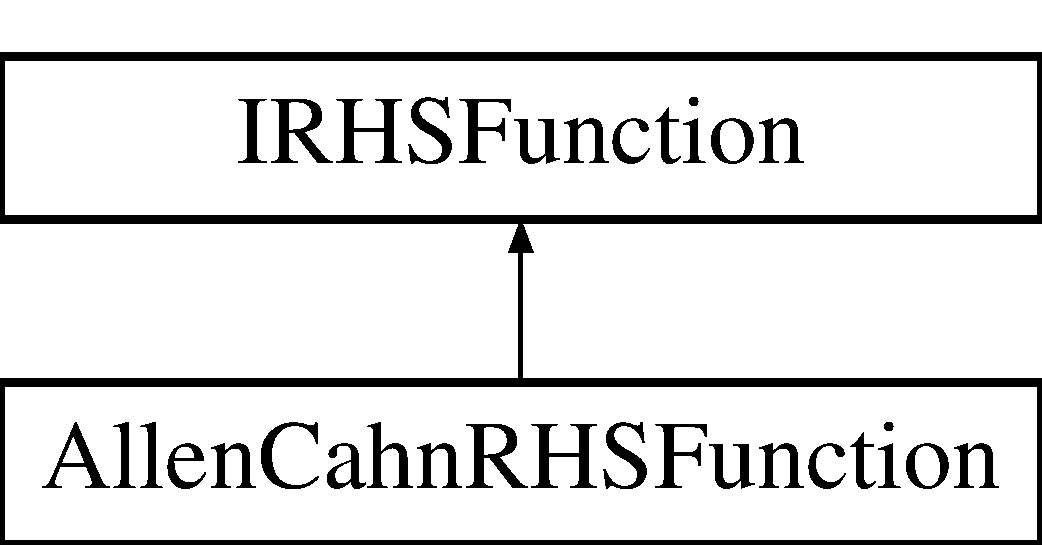
\includegraphics[height=2cm]{classAllenCahnRHSFunction}
\end{center}
\end{figure}
\subsection*{Public Member Functions}
\begin{DoxyCompactItemize}
\item 
\hypertarget{classAllenCahnRHSFunction_adf358cca697faeabd45941ecef135e09}{
void {\bfseries setSigma} (const Real sigma)}
\label{classAllenCahnRHSFunction_adf358cca697faeabd45941ecef135e09}

\item 
\hypertarget{classAllenCahnRHSFunction_a644e239104dc69ab10d24911f65aa0f4}{
void {\bfseries setNx} (const Integer nx)}
\label{classAllenCahnRHSFunction_a644e239104dc69ab10d24911f65aa0f4}

\item 
\hypertarget{classAllenCahnRHSFunction_a74971f71276e33081609df6e2bf7e957}{
Real {\bfseries getSigma} ()}
\label{classAllenCahnRHSFunction_a74971f71276e33081609df6e2bf7e957}

\item 
\hypertarget{classAllenCahnRHSFunction_a67c6edb359ecaec56aa5d04aa4eac183}{
Integer {\bfseries getNx} ()}
\label{classAllenCahnRHSFunction_a67c6edb359ecaec56aa5d04aa4eac183}

\item 
\hypertarget{classAllenCahnRHSFunction_a23944f60ddc12bd00d5afcfac74b4862}{
Real {\bfseries getX0} () const }
\label{classAllenCahnRHSFunction_a23944f60ddc12bd00d5afcfac74b4862}

\item 
\hypertarget{classAllenCahnRHSFunction_a1a495b29623fc793b9021d5448fda2ea}{
void {\bfseries setX0} (Real x0)}
\label{classAllenCahnRHSFunction_a1a495b29623fc793b9021d5448fda2ea}

\item 
\hypertarget{classAllenCahnRHSFunction_a1b2f18b0027c7bca2dd131e7879e228e}{
Real {\bfseries getXL} () const }
\label{classAllenCahnRHSFunction_a1b2f18b0027c7bca2dd131e7879e228e}

\item 
\hypertarget{classAllenCahnRHSFunction_aed5c92e6d1d0add2ff9023547c29a2ed}{
void {\bfseries setXL} (Real l)}
\label{classAllenCahnRHSFunction_aed5c92e6d1d0add2ff9023547c29a2ed}

\item 
RealVector \hyperlink{classAllenCahnRHSFunction_a88cc6858ebc041f62edf9b3fc0505849}{evalF} (Real time, RealVector \&y)
\begin{DoxyCompactList}\small\item\em Returns a vector that it is the RHS evaluated at a certain time and solution. \item\end{DoxyCompactList}\item 
RealVector \hyperlink{classAllenCahnRHSFunction_a4f2df77dfae069945cc40dc2b1eb0200}{evalF} (Real time, RealVector \&y, IntegerVector \&ref)
\begin{DoxyCompactList}\small\item\em Returns a vector that it is the RHS evaluated at a certain time and solution only for the active components. \item\end{DoxyCompactList}\item 
RealMatrixSparse \hyperlink{classAllenCahnRHSFunction_ac203ad1a188d842e6a9a9e70762b2b30}{evaldFdY} (Real time, RealVector \&y)
\begin{DoxyCompactList}\small\item\em Returns the Jacobian matrix at a certain time and solution. \item\end{DoxyCompactList}\item 
RealMatrixSparse \hyperlink{classAllenCahnRHSFunction_a51d138b3083af6914800d956171dfa6a}{evaldFdY} (Real time, RealVector \&y, IntegerVector \&ref)
\begin{DoxyCompactList}\small\item\em Returns the Jacobian matrix at a certain time and solution only for the active components. \item\end{DoxyCompactList}\end{DoxyCompactItemize}


\subsection{Detailed Description}
Class for RHS of PDE $ \frac{\partial u}{ \partial t} = \sigma * \frac{\partial^{2}u}{\partial x^{2} + u(1-(u^{2}))} \frac{\partial u(x0,t)}{ \partial x} = 0; \frac{\partial u(xL,t)}{ \partial x} = 0; $ 

\subsection{Member Function Documentation}
\hypertarget{classAllenCahnRHSFunction_a51d138b3083af6914800d956171dfa6a}{
\index{AllenCahnRHSFunction@{AllenCahnRHSFunction}!evaldFdY@{evaldFdY}}
\index{evaldFdY@{evaldFdY}!AllenCahnRHSFunction@{AllenCahnRHSFunction}}
\subsubsection[{evaldFdY}]{\setlength{\rightskip}{0pt plus 5cm}RealMatrixSparse AllenCahnRHSFunction::evaldFdY (Real {\em time}, \/  RealVector \& {\em y}, \/  IntegerVector \& {\em ref})\hspace{0.3cm}{\ttfamily  \mbox{[}virtual\mbox{]}}}}
\label{classAllenCahnRHSFunction_a51d138b3083af6914800d956171dfa6a}


Returns the Jacobian matrix at a certain time and solution only for the active components. 

this is not the analytical Jacobian! It is compute with finite differences. 

Implements \hyperlink{classIRHSFunction}{IRHSFunction}.\hypertarget{classAllenCahnRHSFunction_ac203ad1a188d842e6a9a9e70762b2b30}{
\index{AllenCahnRHSFunction@{AllenCahnRHSFunction}!evaldFdY@{evaldFdY}}
\index{evaldFdY@{evaldFdY}!AllenCahnRHSFunction@{AllenCahnRHSFunction}}
\subsubsection[{evaldFdY}]{\setlength{\rightskip}{0pt plus 5cm}RealMatrixSparse AllenCahnRHSFunction::evaldFdY (Real {\em time}, \/  RealVector \& {\em y})\hspace{0.3cm}{\ttfamily  \mbox{[}virtual\mbox{]}}}}
\label{classAllenCahnRHSFunction_ac203ad1a188d842e6a9a9e70762b2b30}


Returns the Jacobian matrix at a certain time and solution. 

this is not the analytical Jacobian! It is compute with finite differences. 

Implements \hyperlink{classIRHSFunction}{IRHSFunction}.\hypertarget{classAllenCahnRHSFunction_a4f2df77dfae069945cc40dc2b1eb0200}{
\index{AllenCahnRHSFunction@{AllenCahnRHSFunction}!evalF@{evalF}}
\index{evalF@{evalF}!AllenCahnRHSFunction@{AllenCahnRHSFunction}}
\subsubsection[{evalF}]{\setlength{\rightskip}{0pt plus 5cm}RealVector AllenCahnRHSFunction::evalF (Real {\em time}, \/  RealVector \& {\em y}, \/  IntegerVector \& {\em ref})\hspace{0.3cm}{\ttfamily  \mbox{[}virtual\mbox{]}}}}
\label{classAllenCahnRHSFunction_a4f2df77dfae069945cc40dc2b1eb0200}


Returns a vector that it is the RHS evaluated at a certain time and solution only for the active components. 

For the first and the last node we have to use the Neumann boundary conditions! For the other nodes we use centered finite differences. Only for the components that we have to compute the solution and are not interpolated.

Implements \hyperlink{classIRHSFunction}{IRHSFunction}.\hypertarget{classAllenCahnRHSFunction_a88cc6858ebc041f62edf9b3fc0505849}{
\index{AllenCahnRHSFunction@{AllenCahnRHSFunction}!evalF@{evalF}}
\index{evalF@{evalF}!AllenCahnRHSFunction@{AllenCahnRHSFunction}}
\subsubsection[{evalF}]{\setlength{\rightskip}{0pt plus 5cm}RealVector AllenCahnRHSFunction::evalF (Real {\em time}, \/  RealVector \& {\em y})\hspace{0.3cm}{\ttfamily  \mbox{[}virtual\mbox{]}}}}
\label{classAllenCahnRHSFunction_a88cc6858ebc041f62edf9b3fc0505849}


Returns a vector that it is the RHS evaluated at a certain time and solution. 

I create a uniform grid with Nx nodes.

For the first and the last node we have to use the Neumann boundary conditions! For the other nodes we use centered finite differences.

Implements \hyperlink{classIRHSFunction}{IRHSFunction}.

The documentation for this class was generated from the following files:\begin{DoxyCompactItemize}
\item 
AllenCahnRHSFunction/AllenCahnRHSFunction.h\item 
AllenCahnRHSFunction/AllenCahnRHSFunction.cpp\end{DoxyCompactItemize}

\hypertarget{classRestab_1_1Array}{
\section{Restab::Array$<$ T $>$ Class Template Reference}
\label{classRestab_1_1Array}\index{Restab::Array@{Restab::Array}}
}
\subsection*{Public Member Functions}
\begin{DoxyCompactItemize}
\item 
\hypertarget{classRestab_1_1Array_a53628d891f39d798b1c7f7d0ab2fde4f}{
void {\bfseries add} (T t)}
\label{classRestab_1_1Array_a53628d891f39d798b1c7f7d0ab2fde4f}

\item 
\hypertarget{classRestab_1_1Array_a6d744a9c92c6a8aa761fd46d40ae684e}{
T {\bfseries get} (Integer i)}
\label{classRestab_1_1Array_a6d744a9c92c6a8aa761fd46d40ae684e}

\end{DoxyCompactItemize}
\subsubsection*{template$<$class T$>$ class Restab::Array$<$ T $>$}



The documentation for this class was generated from the following file:\begin{DoxyCompactItemize}
\item 
Restab.h\end{DoxyCompactItemize}

\hypertarget{classBasicNewtonSolver}{
\section{BasicNewtonSolver Class Reference}
\label{classBasicNewtonSolver}\index{BasicNewtonSolver@{BasicNewtonSolver}}
}
Inheritance diagram for BasicNewtonSolver::\begin{figure}[H]
\begin{center}
\leavevmode
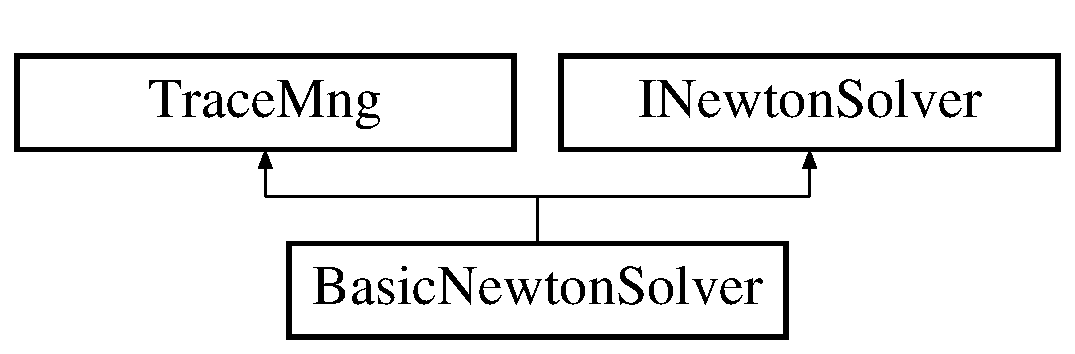
\includegraphics[height=2cm]{classBasicNewtonSolver}
\end{center}
\end{figure}
\subsection*{Public Member Functions}
\begin{DoxyCompactItemize}
\item 
void \hyperlink{classBasicNewtonSolver_a24d27f55e338412dbd6337087a25190a}{compute} (\hyperlink{classINewtonFunction}{INewtonFunction} \&fun, RealMatrixSparse \&J, RealVector \&Y, const Real tol\_\-rel, const Real tol\_\-abs, Bool \&diverge\_\-Newton, const Integer MaxNewtonStep)
\begin{DoxyCompactList}\small\item\em Function to compute the solution with the Newton method for non linear system. \item\end{DoxyCompactList}\end{DoxyCompactItemize}


\subsection{Member Function Documentation}
\hypertarget{classBasicNewtonSolver_a24d27f55e338412dbd6337087a25190a}{
\index{BasicNewtonSolver@{BasicNewtonSolver}!compute@{compute}}
\index{compute@{compute}!BasicNewtonSolver@{BasicNewtonSolver}}
\subsubsection[{compute}]{\setlength{\rightskip}{0pt plus 5cm}void BasicNewtonSolver::compute ({\bf INewtonFunction} \& {\em fun}, \/  RealMatrixSparse \& {\em J}, \/  RealVector \& {\em Y}, \/  const Real {\em tol\_\-rel}, \/  const Real {\em tol\_\-abs}, \/  Bool \& {\em diverge\_\-Newton}, \/  const Integer {\em MaxNewtonStep})\hspace{0.3cm}{\ttfamily  \mbox{[}virtual\mbox{]}}}}
\label{classBasicNewtonSolver_a24d27f55e338412dbd6337087a25190a}


Function to compute the solution with the Newton method for non linear system. Returns the solution by reference 

Implements \hyperlink{classINewtonSolver_aaf2a0a6fbf03d4f58ba24e47590458d0}{INewtonSolver}.

The documentation for this class was generated from the following files:\begin{DoxyCompactItemize}
\item 
NewtonSolver/BasicNewtonSolver.h\item 
NewtonSolver/BasicNewtonSolver.cpp\end{DoxyCompactItemize}

\hypertarget{classBESolver}{
\section{BESolver Class Reference}
\label{classBESolver}\index{BESolver@{BESolver}}
}
Inheritance diagram for BESolver::\begin{figure}[H]
\begin{center}
\leavevmode
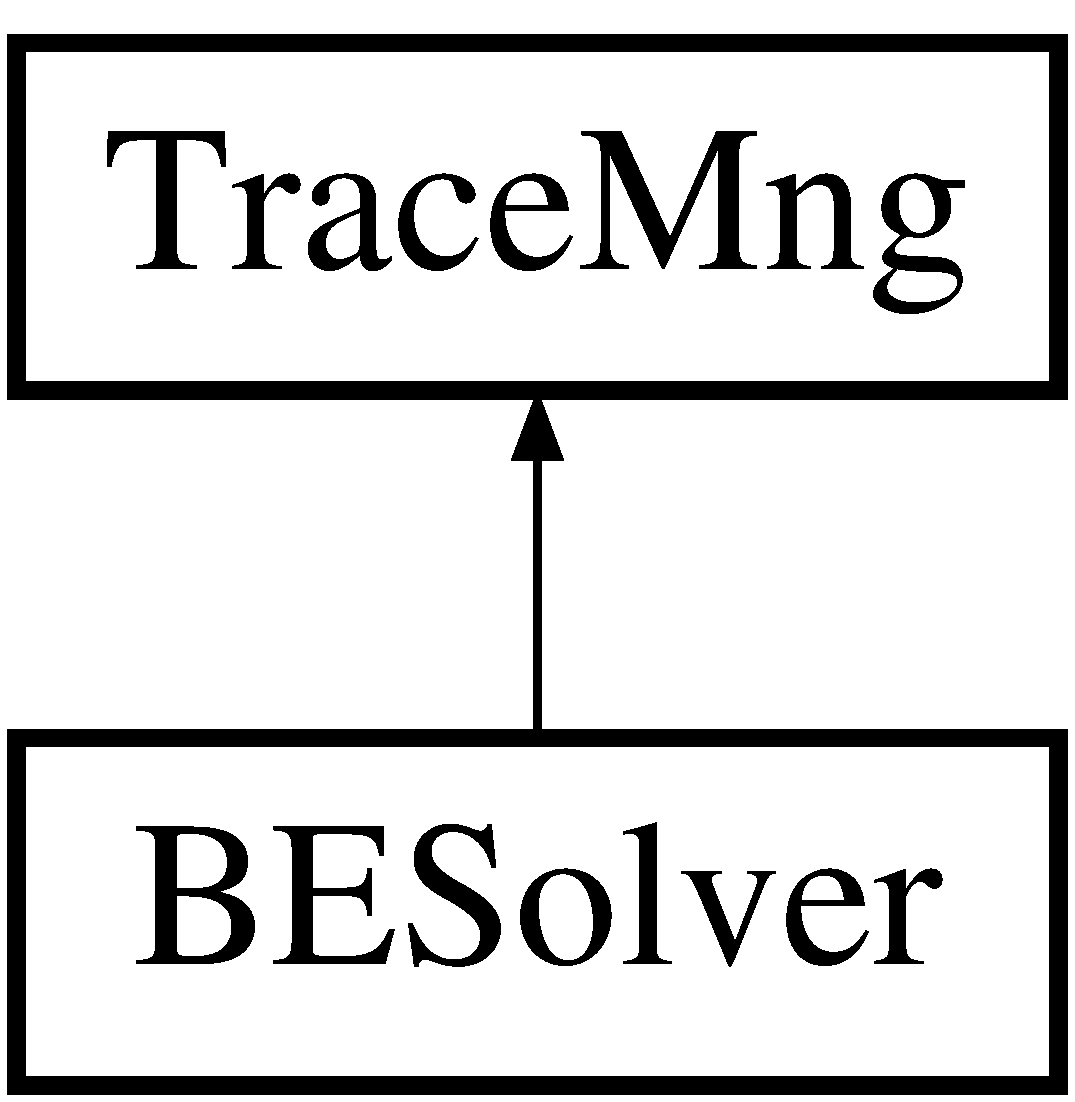
\includegraphics[height=2cm]{classBESolver}
\end{center}
\end{figure}
\subsection*{Public Member Functions}
\begin{DoxyCompactItemize}
\item 
\hypertarget{classBESolver_a75cdcd48861507ea3edd7ebbedf9770c}{
void {\bfseries setRHSFunction} (\hyperlink{classIRHSFunction}{IRHSFunction} $\ast$fun)}
\label{classBESolver_a75cdcd48861507ea3edd7ebbedf9770c}

\item 
\hypertarget{classBESolver_aaf3933d2b810cd9d1da51f9aa9f6e3e3}{
void {\bfseries setNewtSolv} (std::unique\_\-ptr$<$ \hyperlink{classINewtonSolver}{INewtonSolver} $>$ newtSolv)}
\label{classBESolver_aaf3933d2b810cd9d1da51f9aa9f6e3e3}

\item 
\hypertarget{classBESolver_abd9f73ecfe190b8007aed57aeec611ca}{
void \hyperlink{classBESolver_abd9f73ecfe190b8007aed57aeec611ca}{compute} ()}
\label{classBESolver_abd9f73ecfe190b8007aed57aeec611ca}

\begin{DoxyCompactList}\small\item\em This method advances by one time step the solution. \item\end{DoxyCompactList}\item 
\hypertarget{classBESolver_aac67d1152ce69e297e70f520619420b2}{
void {\bfseries setInput} (\hyperlink{classBESolverInput}{BESolverInput} input)}
\label{classBESolver_aac67d1152ce69e297e70f520619420b2}

\item 
\hypertarget{classBESolver_a127b8c23946822caf9ce4e46bce779ab}{
\hyperlink{classBESolverOutput}{BESolverOutput} {\bfseries getOutputBE} ()}
\label{classBESolver_a127b8c23946822caf9ce4e46bce779ab}

\end{DoxyCompactItemize}


The documentation for this class was generated from the following files:\begin{DoxyCompactItemize}
\item 
BESolver/BESolver.h\item 
BESolver/BESolver.cpp\end{DoxyCompactItemize}

\hypertarget{classBESolverInput}{
\section{BESolverInput Class Reference}
\label{classBESolverInput}\index{BESolverInput@{BESolverInput}}
}
\subsection*{Public Member Functions}
\begin{DoxyCompactItemize}
\item 
void \hyperlink{classBESolverInput_ae169118cebc5cab39af09d11eea4aff1}{set} (Real t0, Real dt, RealVector \&y0, Real Newton\_\-tol\_\-rel, Real Newton\_\-tol\_\-abs)
\begin{DoxyCompactList}\small\item\em Sets the input. \item\end{DoxyCompactList}\item 
\hypertarget{classBESolverInput_af7564a03a9212a553fc7308daf91dcfc}{
Real {\bfseries getDt} () const }
\label{classBESolverInput_af7564a03a9212a553fc7308daf91dcfc}

\item 
\hypertarget{classBESolverInput_a058be78d49b73876d0d09a5298c10fbb}{
Real {\bfseries getT0} () const }
\label{classBESolverInput_a058be78d49b73876d0d09a5298c10fbb}

\item 
\hypertarget{classBESolverInput_aae6968751afbbaae823b1f2f35d77ad2}{
RealVector \& {\bfseries getY0} ()}
\label{classBESolverInput_aae6968751afbbaae823b1f2f35d77ad2}

\item 
\hypertarget{classBESolverInput_ab3e74a57ff02d7bd7fe1082cf5d74f09}{
Real {\bfseries getNewtonTolAbs} () const }
\label{classBESolverInput_ab3e74a57ff02d7bd7fe1082cf5d74f09}

\item 
\hypertarget{classBESolverInput_a02df3d117faf378369713a9f9e2aeb60}{
Real {\bfseries getNewtonTolRel} () const }
\label{classBESolverInput_a02df3d117faf378369713a9f9e2aeb60}

\end{DoxyCompactItemize}


\subsection{Member Function Documentation}
\hypertarget{classBESolverInput_ae169118cebc5cab39af09d11eea4aff1}{
\index{BESolverInput@{BESolverInput}!set@{set}}
\index{set@{set}!BESolverInput@{BESolverInput}}
\subsubsection[{set}]{\setlength{\rightskip}{0pt plus 5cm}void BESolverInput::set (Real {\em t0}, \/  Real {\em dt}, \/  RealVector \& {\em y0}, \/  Real {\em Newton\_\-tol\_\-rel}, \/  Real {\em Newton\_\-tol\_\-abs})}}
\label{classBESolverInput_ae169118cebc5cab39af09d11eea4aff1}


Sets the input. 
\begin{DoxyParams}{Parameters}
\item[{\em t0}]initial time \item[{\em dt}]time step \item[{\em y0}]initial solution \item[{\em Newton\_\-tol\_\-rel}]Newton relative tolerance \item[{\em Newton\_\-tol\_\-abs}]Newton absolute tolerance \end{DoxyParams}


The documentation for this class was generated from the following files:\begin{DoxyCompactItemize}
\item 
BESolver/BESolverInput.h\item 
BESolver/BESolverInput.cpp\end{DoxyCompactItemize}

\hypertarget{classBESolverNewtonFunction}{
\section{BESolverNewtonFunction Class Reference}
\label{classBESolverNewtonFunction}\index{BESolverNewtonFunction@{BESolverNewtonFunction}}
}


Newton Function for BE Solver.  


{\ttfamily \#include $<$BESolverNewtonFunction.h$>$}Inheritance diagram for BESolverNewtonFunction::\begin{figure}[H]
\begin{center}
\leavevmode
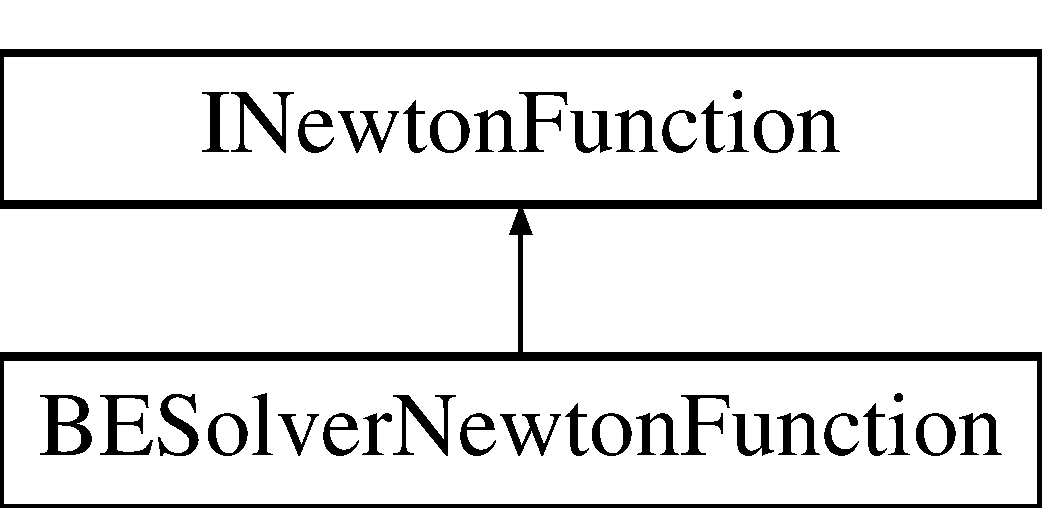
\includegraphics[height=2cm]{classBESolverNewtonFunction}
\end{center}
\end{figure}
\subsection*{Public Member Functions}
\begin{DoxyCompactItemize}
\item 
\hypertarget{classBESolverNewtonFunction_a4839e9f396001ec74f0ed84c60bceeea}{
void {\bfseries setDt} (Real dt)}
\label{classBESolverNewtonFunction_a4839e9f396001ec74f0ed84c60bceeea}

\item 
\hypertarget{classBESolverNewtonFunction_af8ac5afaee7f9150715d64864113728f}{
void {\bfseries setFun} (\hyperlink{classIRHSFunction}{IRHSFunction} $\ast$fun)}
\label{classBESolverNewtonFunction_af8ac5afaee7f9150715d64864113728f}

\item 
\hypertarget{classBESolverNewtonFunction_a6a0988dcce895a7da36f33adaa412a0c}{
void {\bfseries setYn} (const RealVector \&yn)}
\label{classBESolverNewtonFunction_a6a0988dcce895a7da36f33adaa412a0c}

\item 
\hypertarget{classBESolverNewtonFunction_a8120d01800736505481b08e47394fe84}{
void {\bfseries setTnp} (Real tnp)}
\label{classBESolverNewtonFunction_a8120d01800736505481b08e47394fe84}

\item 
\hypertarget{classBESolverNewtonFunction_aab571de51fc3667739191c93df8a0065}{
void \hyperlink{classBESolverNewtonFunction_aab571de51fc3667739191c93df8a0065}{evalFJ} (RealVector \&Y, RealVector \&F, RealMatrixSparse \&J)}
\label{classBESolverNewtonFunction_aab571de51fc3667739191c93df8a0065}

\begin{DoxyCompactList}\small\item\em Returns as references the evaluate of Newton function (F) and Newton Jacobian (J) in Y. \item\end{DoxyCompactList}\item 
\hypertarget{classBESolverNewtonFunction_a66238e6376f8ec8945a3867b3a065deb}{
void \hyperlink{classBESolverNewtonFunction_a66238e6376f8ec8945a3867b3a065deb}{evalF} (RealVector \&Y, RealVector \&F)}
\label{classBESolverNewtonFunction_a66238e6376f8ec8945a3867b3a065deb}

\begin{DoxyCompactList}\small\item\em Returns as reference the evaluate of Newton function (F) in Y. \item\end{DoxyCompactList}\end{DoxyCompactItemize}


\subsection{Detailed Description}
Newton Function for BE Solver. $ F(y) = y - y_{n} - dt*(f_{RHS}(t_{n+1},y)) $ 

The documentation for this class was generated from the following files:\begin{DoxyCompactItemize}
\item 
BESolverNewtonFunction/BESolverNewtonFunction.h\item 
BESolverNewtonFunction/BESolverNewtonFunction.cpp\end{DoxyCompactItemize}

\hypertarget{classBESolverOutput}{
\section{BESolverOutput Class Reference}
\label{classBESolverOutput}\index{BESolverOutput@{BESolverOutput}}
}


Output for the time step solver.  


{\ttfamily \#include $<$BESolverOutput.h$>$}\subsection*{Public Member Functions}
\begin{DoxyCompactItemize}
\item 
\hypertarget{classBESolverOutput_af64510e72c2be3c1893dcf860cb2f59f}{
void {\bfseries setYFinal} (const RealVector \&final)}
\label{classBESolverOutput_af64510e72c2be3c1893dcf860cb2f59f}

\item 
\hypertarget{classBESolverOutput_a65170df7854de381abfeeda76476d6a3}{
const RealVector \& {\bfseries getYFinal} () const }
\label{classBESolverOutput_a65170df7854de381abfeeda76476d6a3}

\item 
\hypertarget{classBESolverOutput_ab010f2b70af2ddde1d932dcae2885abd}{
Real {\bfseries getTFinal} () const }
\label{classBESolverOutput_ab010f2b70af2ddde1d932dcae2885abd}

\item 
\hypertarget{classBESolverOutput_a2f0275ab6bc4dab947926375a45c7e07}{
Bool {\bfseries getIsConverged} () const }
\label{classBESolverOutput_a2f0275ab6bc4dab947926375a45c7e07}

\item 
\hypertarget{classBESolverOutput_a78b7246f32c4a733af2bb0e92c6d7f4c}{
void {\bfseries setIsConverged} (Bool isConverged)}
\label{classBESolverOutput_a78b7246f32c4a733af2bb0e92c6d7f4c}

\item 
\hypertarget{classBESolverOutput_ad6a51456e274386d290d8614aa42b835}{
void {\bfseries setTFinal} (const Real final)}
\label{classBESolverOutput_ad6a51456e274386d290d8614aa42b835}

\item 
\hypertarget{classBESolverOutput_afdafc1ea0c5363efa4ac203f4f6e9c8f}{
Real {\bfseries getDt} () const }
\label{classBESolverOutput_afdafc1ea0c5363efa4ac203f4f6e9c8f}

\item 
\hypertarget{classBESolverOutput_a7f1f43b10a953825a95475d99270626e}{
void {\bfseries setDt} (Real dt)}
\label{classBESolverOutput_a7f1f43b10a953825a95475d99270626e}

\end{DoxyCompactItemize}


\subsection{Detailed Description}
Output for the time step solver. 

The documentation for this class was generated from the following files:\begin{DoxyCompactItemize}
\item 
BESolver/BESolverOutput.h\item 
BESolver/BESolverOutput.cpp\end{DoxyCompactItemize}

\hypertarget{classBESolverUtils}{
\section{BESolverUtils Class Reference}
\label{classBESolverUtils}\index{BESolverUtils@{BESolverUtils}}
}
Inheritance diagram for BESolverUtils::\begin{figure}[H]
\begin{center}
\leavevmode
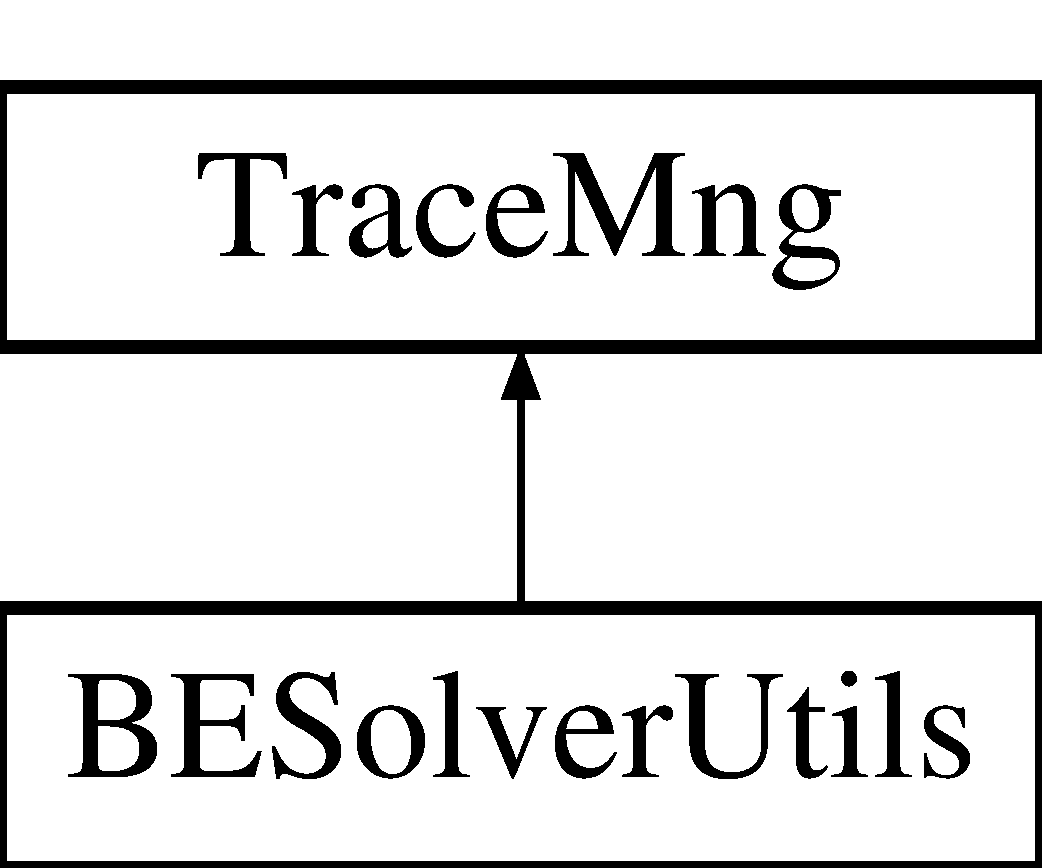
\includegraphics[height=2cm]{classBESolverUtils}
\end{center}
\end{figure}
\subsection*{Public Member Functions}
\begin{DoxyCompactItemize}
\item 
\hypertarget{classBESolverUtils_a4229f6f6ac615a46c073c3359f1e1150}{
void \hyperlink{classBESolverUtils_a4229f6f6ac615a46c073c3359f1e1150}{printInfo} (\hyperlink{classBESolverOutput}{BESolverOutput} output)}
\label{classBESolverUtils_a4229f6f6ac615a46c073c3359f1e1150}

\begin{DoxyCompactList}\small\item\em Outputs some info on the time step solver. \item\end{DoxyCompactList}\end{DoxyCompactItemize}


The documentation for this class was generated from the following files:\begin{DoxyCompactItemize}
\item 
BESolver/BESolverUtils.h\item 
BESolver/BESolverUtils.cpp\end{DoxyCompactItemize}

\hypertarget{classBurgersFluxFunction}{
\section{BurgersFluxFunction Class Reference}
\label{classBurgersFluxFunction}\index{BurgersFluxFunction@{BurgersFluxFunction}}
}
Inheritance diagram for BurgersFluxFunction::\begin{figure}[H]
\begin{center}
\leavevmode
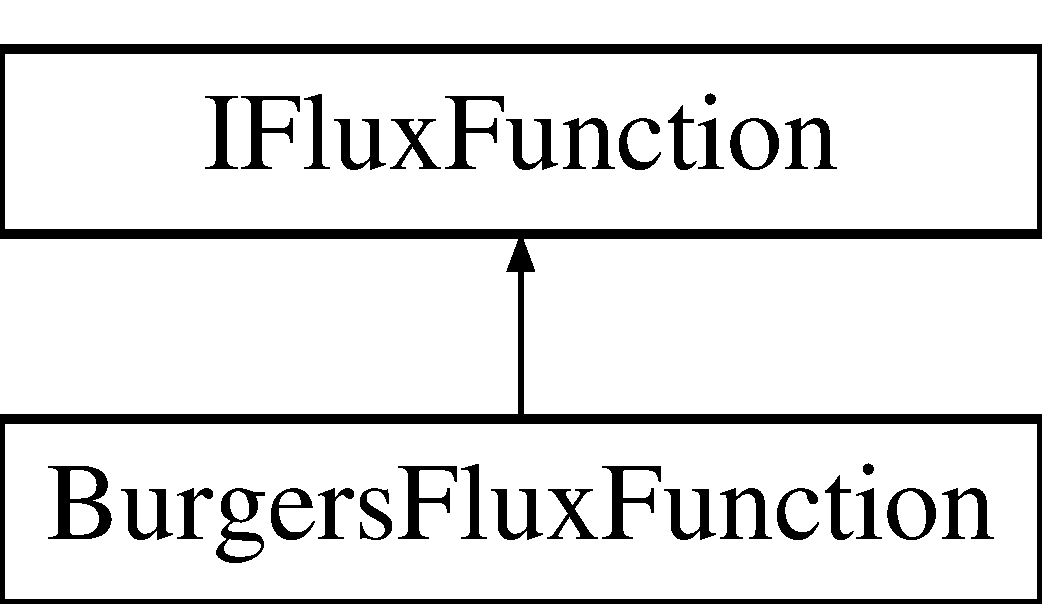
\includegraphics[height=2cm]{classBurgersFluxFunction}
\end{center}
\end{figure}
\subsection*{Public Member Functions}
\begin{DoxyCompactItemize}
\item 
\hypertarget{classBurgersFluxFunction_a89fdd1c6cc40707e2a83701eda1777d0}{
Real {\bfseries evalF} (Real time, Real y\_\-sol)}
\label{classBurgersFluxFunction_a89fdd1c6cc40707e2a83701eda1777d0}

\item 
\hypertarget{classBurgersFluxFunction_ad86ece8a9bf4750a6159311390efa6cd}{
Real {\bfseries evalFderivative} (Real time, Real y\_\-sol)}
\label{classBurgersFluxFunction_ad86ece8a9bf4750a6159311390efa6cd}

\end{DoxyCompactItemize}


The documentation for this class was generated from the following files:\begin{DoxyCompactItemize}
\item 
HyperbolicEquationRusanovFlux/BurgersFluxFunction.h\item 
HyperbolicEquationRusanovFlux/BurgersFluxFunction.cpp\end{DoxyCompactItemize}

\hypertarget{classChemicalPhase}{
\section{ChemicalPhase Class Reference}
\label{classChemicalPhase}\index{ChemicalPhase@{ChemicalPhase}}
}
\subsection*{Public Member Functions}
\begin{DoxyCompactItemize}
\item 
\hypertarget{classChemicalPhase_aa73ef3b78a5dab9bffae03173a3f9d70}{
{\bfseries ChemicalPhase} (String phase, String phaseModel, String law)}
\label{classChemicalPhase_aa73ef3b78a5dab9bffae03173a3f9d70}

\item 
\hypertarget{classChemicalPhase_a23fc0a2d0d84959d653b2913ced12ed9}{
void {\bfseries setChemicalPhase} (String phase, String phaseModel, String law)}
\label{classChemicalPhase_a23fc0a2d0d84959d653b2913ced12ed9}

\item 
\hypertarget{classChemicalPhase_a46d6d3c2fb58213b8decaae5e5542a35}{
const String \& {\bfseries getLaw} () const }
\label{classChemicalPhase_a46d6d3c2fb58213b8decaae5e5542a35}

\item 
\hypertarget{classChemicalPhase_ad1dd0dc5eb3bbb4edaf5f83c43d1778c}{
const String \& {\bfseries getPhase} () const }
\label{classChemicalPhase_ad1dd0dc5eb3bbb4edaf5f83c43d1778c}

\item 
\hypertarget{classChemicalPhase_a81624aa6a6b8201ab2fd336a8be8466e}{
const String \& {\bfseries getPhaseModel} () const }
\label{classChemicalPhase_a81624aa6a6b8201ab2fd336a8be8466e}

\end{DoxyCompactItemize}


The documentation for this class was generated from the following files:\begin{DoxyCompactItemize}
\item 
ChemicalSystemTools/ChemicalPhase.h\item 
ChemicalSystemTools/ChemicalPhase.cpp\end{DoxyCompactItemize}

\hypertarget{classChemicalReaction}{
\section{ChemicalReaction Class Reference}
\label{classChemicalReaction}\index{ChemicalReaction@{ChemicalReaction}}
}
\subsection*{Public Member Functions}
\begin{DoxyCompactItemize}
\item 
\hypertarget{classChemicalReaction_a6af90fdc570a3b58f983b7cf9692e766}{
{\bfseries ChemicalReaction} (String nameReaction, Real kinValue)}
\label{classChemicalReaction_a6af90fdc570a3b58f983b7cf9692e766}

\item 
\hypertarget{classChemicalReaction_a31a0d6302796ce560d2983d7885f2c0d}{
void {\bfseries setChemicalReaction} (String nameReaction, Real kinValue)}
\label{classChemicalReaction_a31a0d6302796ce560d2983d7885f2c0d}

\item 
\hypertarget{classChemicalReaction_a6a8e09e4c96dc351fdb756ff4848e35f}{
void {\bfseries addSpecies} (KeyReal species)}
\label{classChemicalReaction_a6a8e09e4c96dc351fdb756ff4848e35f}

\item 
\hypertarget{classChemicalReaction_a2bc0c065a07adba9c2f97d69052d91ee}{
const String \& {\bfseries getNameReaction} () const }
\label{classChemicalReaction_a2bc0c065a07adba9c2f97d69052d91ee}

\item 
\hypertarget{classChemicalReaction_ac4b8b5ae5d9b806d7e37323876f3081c}{
Real {\bfseries getKinValue} () const }
\label{classChemicalReaction_ac4b8b5ae5d9b806d7e37323876f3081c}

\item 
\hypertarget{classChemicalReaction_ae00e74e62e03e4bb642b5bcce178ff5e}{
const std::vector$<$ KeyReal $>$ \& {\bfseries getSpecies} () const }
\label{classChemicalReaction_ae00e74e62e03e4bb642b5bcce178ff5e}

\end{DoxyCompactItemize}


The documentation for this class was generated from the following files:\begin{DoxyCompactItemize}
\item 
ChemicalSystemTools/ChemicalReaction.h\item 
ChemicalSystemTools/ChemicalReaction.cpp\end{DoxyCompactItemize}

\hypertarget{classChemicalSourceRate}{
\section{ChemicalSourceRate Class Reference}
\label{classChemicalSourceRate}\index{ChemicalSourceRate@{ChemicalSourceRate}}
}
\subsection*{Public Member Functions}
\begin{DoxyCompactItemize}
\item 
\hypertarget{classChemicalSourceRate_a4ae0590def527e09a4c4ba19562c4ea7}{
void {\bfseries setSourceRate} (KeyReal sourceRate)}
\label{classChemicalSourceRate_a4ae0590def527e09a4c4ba19562c4ea7}

\item 
\hypertarget{classChemicalSourceRate_a53dfd88295b2211a4c40aa8b51691c73}{
const std::vector$<$ KeyReal $>$ \& {\bfseries getSourceRate} () const }
\label{classChemicalSourceRate_a53dfd88295b2211a4c40aa8b51691c73}

\end{DoxyCompactItemize}


The documentation for this class was generated from the following files:\begin{DoxyCompactItemize}
\item 
ChemicalSystemTools/ChemicalSourceRate.h\item 
ChemicalSystemTools/ChemicalSourceRate.cpp\end{DoxyCompactItemize}

\hypertarget{classChemicalSpecies}{
\section{ChemicalSpecies Class Reference}
\label{classChemicalSpecies}\index{ChemicalSpecies@{ChemicalSpecies}}
}
\subsection*{Public Member Functions}
\begin{DoxyCompactItemize}
\item 
\hypertarget{classChemicalSpecies_a72ccba3bec44166dedc0b203b3528703}{
{\bfseries ChemicalSpecies} (String species, String speciesPhase, String speciesModel, String sModel, Real logk)}
\label{classChemicalSpecies_a72ccba3bec44166dedc0b203b3528703}

\item 
\hypertarget{classChemicalSpecies_a8f89b95c5f47214080cb18c8b4d542da}{
void {\bfseries setChemicalSpecies} (String species, String speciesPhase, String speciesModel, String sModel, Real logk)}
\label{classChemicalSpecies_a8f89b95c5f47214080cb18c8b4d542da}

\item 
\hypertarget{classChemicalSpecies_ab7ad83f095e2a4f1fc258ce2518f342a}{
Real {\bfseries getLogk} () const }
\label{classChemicalSpecies_ab7ad83f095e2a4f1fc258ce2518f342a}

\item 
\hypertarget{classChemicalSpecies_a60d41b98d78a8e9ef5daa6c9b32ae6b6}{
const String \& {\bfseries getSModel} () const }
\label{classChemicalSpecies_a60d41b98d78a8e9ef5daa6c9b32ae6b6}

\item 
\hypertarget{classChemicalSpecies_a970db2293bf68bfc277e2bfb9114dd8e}{
const String \& {\bfseries getSpecies} () const }
\label{classChemicalSpecies_a970db2293bf68bfc277e2bfb9114dd8e}

\item 
\hypertarget{classChemicalSpecies_a12fda065e554be6b54ff324939c5bd1b}{
const String \& {\bfseries getSpeciesModel} () const }
\label{classChemicalSpecies_a12fda065e554be6b54ff324939c5bd1b}

\item 
\hypertarget{classChemicalSpecies_a7a44f124badcf1ba81a0463a3cb04916}{
const String \& {\bfseries getSpeciesPhase} () const }
\label{classChemicalSpecies_a7a44f124badcf1ba81a0463a3cb04916}

\end{DoxyCompactItemize}


The documentation for this class was generated from the following files:\begin{DoxyCompactItemize}
\item 
ChemicalSystemTools/ChemicalSpecies.h\item 
ChemicalSystemTools/ChemicalSpecies.cpp\end{DoxyCompactItemize}

\hypertarget{classChemicalSystem}{
\section{ChemicalSystem Class Reference}
\label{classChemicalSystem}\index{ChemicalSystem@{ChemicalSystem}}
}
\subsection*{Public Member Functions}
\begin{DoxyCompactItemize}
\item 
\hypertarget{classChemicalSystem_af5329cab016edc282c8c9649bfb9e17b}{
const std::vector$<$ \hyperlink{classChemicalPhase}{ChemicalPhase} $>$ \& {\bfseries getPhase} () const }
\label{classChemicalSystem_af5329cab016edc282c8c9649bfb9e17b}

\item 
\hypertarget{classChemicalSystem_a033fb4111d6a7efae0ac2366934a7075}{
const std::vector$<$ \hyperlink{classChemicalReaction}{ChemicalReaction} $>$ \& {\bfseries getReaction} () const }
\label{classChemicalSystem_a033fb4111d6a7efae0ac2366934a7075}

\item 
\hypertarget{classChemicalSystem_ab7390699dc460d3591681608fc1977f9}{
const std::vector$<$ \hyperlink{classChemicalSpecies}{ChemicalSpecies} $>$ \& {\bfseries getSpecies} () const }
\label{classChemicalSystem_ab7390699dc460d3591681608fc1977f9}

\item 
\hypertarget{classChemicalSystem_ab472cd49dfcc13a513c86862718202e9}{
void {\bfseries addPhase} (\hyperlink{classChemicalPhase}{ChemicalPhase} phase)}
\label{classChemicalSystem_ab472cd49dfcc13a513c86862718202e9}

\item 
\hypertarget{classChemicalSystem_a246cc3cd35ac8f22743a37cc0e3df5cf}{
void {\bfseries addSpecies} (\hyperlink{classChemicalSpecies}{ChemicalSpecies} species)}
\label{classChemicalSystem_a246cc3cd35ac8f22743a37cc0e3df5cf}

\item 
\hypertarget{classChemicalSystem_ab28e575a558063b14317fff90984227e}{
void {\bfseries addReaction} (\hyperlink{classChemicalReaction}{ChemicalReaction} reaction)}
\label{classChemicalSystem_ab28e575a558063b14317fff90984227e}

\end{DoxyCompactItemize}


The documentation for this class was generated from the following files:\begin{DoxyCompactItemize}
\item 
ChemicalSystemTools/ChemicalSystem.h\item 
ChemicalSystemTools/ChemicalSystem.cpp\end{DoxyCompactItemize}

\hypertarget{classChemicalSystemState}{
\section{ChemicalSystemState Class Reference}
\label{classChemicalSystemState}\index{ChemicalSystemState@{ChemicalSystemState}}
}
\subsection*{Public Member Functions}
\begin{DoxyCompactItemize}
\item 
\hypertarget{classChemicalSystemState_a90288975cb9a28e55d50851e8a4fd962}{
void {\bfseries setAmountSpecies} (KeyReal stateSpecies)}
\label{classChemicalSystemState_a90288975cb9a28e55d50851e8a4fd962}

\item 
\hypertarget{classChemicalSystemState_a0778859d03b8dde1e9654e17a35b6159}{
const std::vector$<$ KeyReal $>$ \& {\bfseries getStateSpecies} () const }
\label{classChemicalSystemState_a0778859d03b8dde1e9654e17a35b6159}

\end{DoxyCompactItemize}


The documentation for this class was generated from the following files:\begin{DoxyCompactItemize}
\item 
ChemicalSystemTools/ChemicalSystemState.h\item 
ChemicalSystemTools/ChemicalSystemState.cpp\end{DoxyCompactItemize}

\hypertarget{classTimings_1_1Chrono}{
\section{Timings::Chrono Class Reference}
\label{classTimings_1_1Chrono}\index{Timings::Chrono@{Timings::Chrono}}
}
\subsection*{Public Member Functions}
\begin{DoxyCompactItemize}
\item 
\hypertarget{classTimings_1_1Chrono_ad6f26c8e4b1e0835e64111539539f790}{
\hyperlink{classTimings_1_1Chrono_ad6f26c8e4b1e0835e64111539539f790}{Chrono} (const \hyperlink{classTimings_1_1Chrono}{Chrono} \&)}
\label{classTimings_1_1Chrono_ad6f26c8e4b1e0835e64111539539f790}

\begin{DoxyCompactList}\small\item\em Explicitly defaulted automatic consts/assignements. \item\end{DoxyCompactList}\item 
\hypertarget{classTimings_1_1Chrono_a6ec606516a51e26069a8fb954f9f3a17}{
{\bfseries Chrono} (\hyperlink{classTimings_1_1Chrono}{Chrono} \&\&)}
\label{classTimings_1_1Chrono_a6ec606516a51e26069a8fb954f9f3a17}

\item 
\hypertarget{classTimings_1_1Chrono_a849fee8b2d99488eee4e83c774079557}{
\hyperlink{classTimings_1_1Chrono}{Chrono} \& {\bfseries operator=} (\hyperlink{classTimings_1_1Chrono}{Chrono} \&\&)}
\label{classTimings_1_1Chrono_a849fee8b2d99488eee4e83c774079557}

\item 
\hypertarget{classTimings_1_1Chrono_a3a2307eff53e845add3236149cf4ed0b}{
\hyperlink{classTimings_1_1Chrono}{Chrono} \& {\bfseries operator=} (const \hyperlink{classTimings_1_1Chrono}{Chrono} \&)}
\label{classTimings_1_1Chrono_a3a2307eff53e845add3236149cf4ed0b}

\item 
\hypertarget{classTimings_1_1Chrono_aefe8228cdb096ba44351f0cfa729745d}{
void \hyperlink{classTimings_1_1Chrono_aefe8228cdb096ba44351f0cfa729745d}{start} ()}
\label{classTimings_1_1Chrono_aefe8228cdb096ba44351f0cfa729745d}

\begin{DoxyCompactList}\small\item\em Starts/reset counting time. \item\end{DoxyCompactList}\item 
\hypertarget{classTimings_1_1Chrono_a4f3e8cc48b33ec4fa0fe2ef160ca9474}{
void \hyperlink{classTimings_1_1Chrono_a4f3e8cc48b33ec4fa0fe2ef160ca9474}{stop} ()}
\label{classTimings_1_1Chrono_a4f3e8cc48b33ec4fa0fe2ef160ca9474}

\begin{DoxyCompactList}\small\item\em Stops counting time. \item\end{DoxyCompactList}\item 
\hypertarget{classTimings_1_1Chrono_a7072889b8af30d030d9c2ecfd2770771}{
double \hyperlink{classTimings_1_1Chrono_a7072889b8af30d030d9c2ecfd2770771}{wallTime} () const }
\label{classTimings_1_1Chrono_a7072889b8af30d030d9c2ecfd2770771}

\begin{DoxyCompactList}\small\item\em Outputs wall time between last start and stop (in seconds). \item\end{DoxyCompactList}\item 
\hypertarget{classTimings_1_1Chrono_a85a7c55297dd9eefde2487b0ec5e8c1c}{
double \hyperlink{classTimings_1_1Chrono_a85a7c55297dd9eefde2487b0ec5e8c1c}{wallTimeNow} () const }
\label{classTimings_1_1Chrono_a85a7c55297dd9eefde2487b0ec5e8c1c}

\begin{DoxyCompactList}\small\item\em Outputs wall time between last start and now! (in seconds). \item\end{DoxyCompactList}\end{DoxyCompactItemize}
\subsection*{Friends}
\begin{DoxyCompactItemize}
\item 
\hypertarget{classTimings_1_1Chrono_a2b517387193dba843d6ce9a05250a070}{
std::ostream \& \hyperlink{classTimings_1_1Chrono_a2b517387193dba843d6ce9a05250a070}{operator$<$$<$} (std::ostream \&, \hyperlink{classTimings_1_1Chrono}{Chrono} const \&)}
\label{classTimings_1_1Chrono_a2b517387193dba843d6ce9a05250a070}

\begin{DoxyCompactList}\small\item\em Outputs time from last start and stop. \item\end{DoxyCompactList}\end{DoxyCompactItemize}


The documentation for this class was generated from the following files:\begin{DoxyCompactItemize}
\item 
chrono.hpp\item 
chrono.cpp\end{DoxyCompactItemize}

\hypertarget{classConstantBCFunction}{
\section{ConstantBCFunction Class Reference}
\label{classConstantBCFunction}\index{ConstantBCFunction@{ConstantBCFunction}}
}


Class to store the Dirichlet boundary condition for the Hyperbolic PDE.  


{\ttfamily \#include $<$ConstantBCFunction.h$>$}Inheritance diagram for ConstantBCFunction::\begin{figure}[H]
\begin{center}
\leavevmode
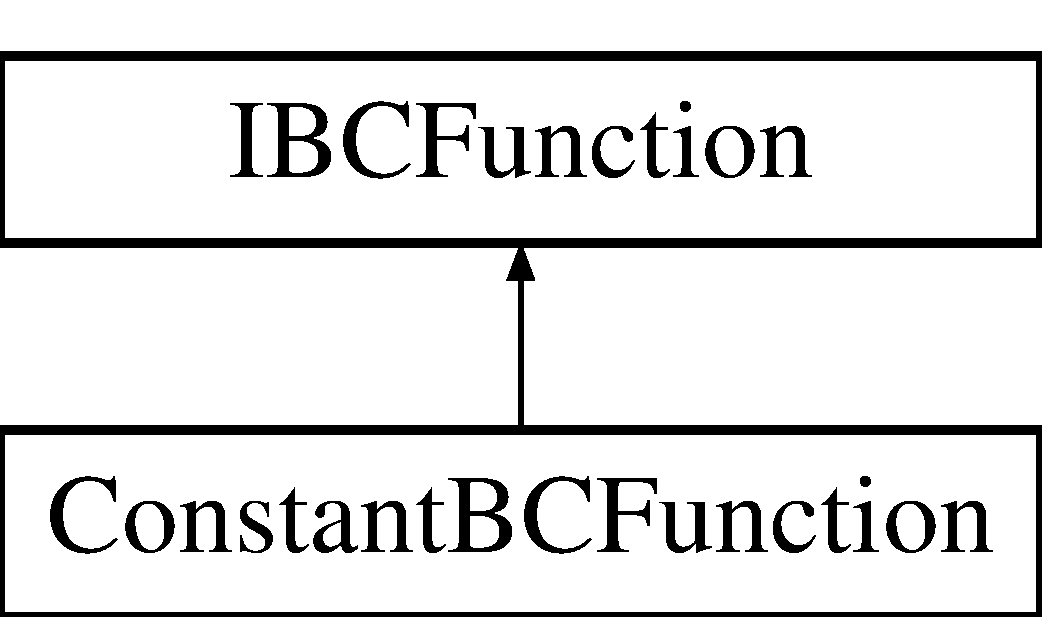
\includegraphics[height=2cm]{classConstantBCFunction}
\end{center}
\end{figure}
\subsection*{Public Member Functions}
\begin{DoxyCompactItemize}
\item 
\hypertarget{classConstantBCFunction_ac8b4e6d431c17a938b26b9ab33dc2245}{
Real {\bfseries getValue} (Real time)}
\label{classConstantBCFunction_ac8b4e6d431c17a938b26b9ab33dc2245}

\item 
\hypertarget{classConstantBCFunction_a061c12e0c2e73b1026035d642092749b}{
void {\bfseries setValue} (Real BCvalue)}
\label{classConstantBCFunction_a061c12e0c2e73b1026035d642092749b}

\end{DoxyCompactItemize}


\subsection{Detailed Description}
Class to store the Dirichlet boundary condition for the Hyperbolic PDE. In this class we have a constant function. 

The documentation for this class was generated from the following files:\begin{DoxyCompactItemize}
\item 
ConstantBCFunction/ConstantBCFunction.h\item 
ConstantBCFunction/ConstantBCFunction.cpp\end{DoxyCompactItemize}

\hypertarget{classCubicHermiteInterpolationInputSolver}{
\section{CubicHermiteInterpolationInputSolver Class Reference}
\label{classCubicHermiteInterpolationInputSolver}\index{CubicHermiteInterpolationInputSolver@{CubicHermiteInterpolationInputSolver}}
}
\subsection*{Public Member Functions}
\begin{DoxyCompactItemize}
\item 
\hypertarget{classCubicHermiteInterpolationInputSolver_af88bf041935f0059d60cbc59d376c562}{
void {\bfseries setRef} (const IntegerVector \&ref)}
\label{classCubicHermiteInterpolationInputSolver_af88bf041935f0059d60cbc59d376c562}

\item 
\hypertarget{classCubicHermiteInterpolationInputSolver_a6595ab2c6bf05d8cac27bf61a15acf3b}{
void {\bfseries setT0Int} (const RealVector \&t0Int)}
\label{classCubicHermiteInterpolationInputSolver_a6595ab2c6bf05d8cac27bf61a15acf3b}

\item 
\hypertarget{classCubicHermiteInterpolationInputSolver_afb1bbd061fa2aee97f98d67d2471ee4d}{
void {\bfseries setT1Int} (const RealVector \&t1Int)}
\label{classCubicHermiteInterpolationInputSolver_afb1bbd061fa2aee97f98d67d2471ee4d}

\item 
\hypertarget{classCubicHermiteInterpolationInputSolver_a939b229acbe2594bf002c3efe4e68c94}{
void {\bfseries setT2Int} (const RealVector \&t2Int)}
\label{classCubicHermiteInterpolationInputSolver_a939b229acbe2594bf002c3efe4e68c94}

\item 
\hypertarget{classCubicHermiteInterpolationInputSolver_a7e38af555ded333308c026ffe9345d53}{
void {\bfseries setY0Int} (const RealVector \&y0Int)}
\label{classCubicHermiteInterpolationInputSolver_a7e38af555ded333308c026ffe9345d53}

\item 
\hypertarget{classCubicHermiteInterpolationInputSolver_a55eb332143a93ecaaa6c6cddbb13be28}{
void {\bfseries setY1Int} (const RealVector \&y1Int)}
\label{classCubicHermiteInterpolationInputSolver_a55eb332143a93ecaaa6c6cddbb13be28}

\item 
\hypertarget{classCubicHermiteInterpolationInputSolver_a46b4dfe81f7e03877dab1984426390ee}{
void {\bfseries setY2Int} (const RealVector \&y2Int)}
\label{classCubicHermiteInterpolationInputSolver_a46b4dfe81f7e03877dab1984426390ee}

\item 
\hypertarget{classCubicHermiteInterpolationInputSolver_ac6392254a279228e4c7f5e29809efdd1}{
void {\bfseries setZ0Int} (const RealVector \&z0Int)}
\label{classCubicHermiteInterpolationInputSolver_ac6392254a279228e4c7f5e29809efdd1}

\item 
\hypertarget{classCubicHermiteInterpolationInputSolver_a8b10728e0da5a3a3b39d9a60725c5d00}{
void {\bfseries setZ1Int} (const RealVector \&z1Int)}
\label{classCubicHermiteInterpolationInputSolver_a8b10728e0da5a3a3b39d9a60725c5d00}

\item 
\hypertarget{classCubicHermiteInterpolationInputSolver_ac42a913883c8be029f8f106de0242c46}{
void {\bfseries setZ2Int} (const RealVector \&z2Int)}
\label{classCubicHermiteInterpolationInputSolver_ac42a913883c8be029f8f106de0242c46}

\item 
\hypertarget{classCubicHermiteInterpolationInputSolver_a723e99edf9560ecdc46b8182e962d274}{
const IntegerVector \& {\bfseries getRef} () const }
\label{classCubicHermiteInterpolationInputSolver_a723e99edf9560ecdc46b8182e962d274}

\item 
\hypertarget{classCubicHermiteInterpolationInputSolver_a996a8c4dcd486b1811acf584a978ea40}{
const RealVector \& {\bfseries getT0Int} () const }
\label{classCubicHermiteInterpolationInputSolver_a996a8c4dcd486b1811acf584a978ea40}

\item 
\hypertarget{classCubicHermiteInterpolationInputSolver_ab701bb75ca8285eda7aeccf653342753}{
const RealVector \& {\bfseries getT1Int} () const }
\label{classCubicHermiteInterpolationInputSolver_ab701bb75ca8285eda7aeccf653342753}

\item 
\hypertarget{classCubicHermiteInterpolationInputSolver_af5ab872432c90aeca491942919faeb20}{
const RealVector \& {\bfseries getT2Int} () const }
\label{classCubicHermiteInterpolationInputSolver_af5ab872432c90aeca491942919faeb20}

\item 
\hypertarget{classCubicHermiteInterpolationInputSolver_a71e6b6dbd8da276544a56b894742488a}{
const RealVector \& {\bfseries getY0Int} () const }
\label{classCubicHermiteInterpolationInputSolver_a71e6b6dbd8da276544a56b894742488a}

\item 
\hypertarget{classCubicHermiteInterpolationInputSolver_ab64418a694f822e0f5246d598061b4ae}{
const RealVector \& {\bfseries getY1Int} () const }
\label{classCubicHermiteInterpolationInputSolver_ab64418a694f822e0f5246d598061b4ae}

\item 
\hypertarget{classCubicHermiteInterpolationInputSolver_ae967f5ec314040184a130353f155246e}{
const RealVector \& {\bfseries getY2Int} () const }
\label{classCubicHermiteInterpolationInputSolver_ae967f5ec314040184a130353f155246e}

\item 
\hypertarget{classCubicHermiteInterpolationInputSolver_a5621da0e021e3c4f1a9bb0191b8644fd}{
const RealVector \& {\bfseries getZ0Int} () const }
\label{classCubicHermiteInterpolationInputSolver_a5621da0e021e3c4f1a9bb0191b8644fd}

\item 
\hypertarget{classCubicHermiteInterpolationInputSolver_ad1671ab8460455a1e35a42e79b2feaf3}{
const RealVector \& {\bfseries getZ1Int} () const }
\label{classCubicHermiteInterpolationInputSolver_ad1671ab8460455a1e35a42e79b2feaf3}

\item 
\hypertarget{classCubicHermiteInterpolationInputSolver_af04cbd96ed2cd9a38c9cc00194aa150f}{
const RealVector \& {\bfseries getZ2Int} () const }
\label{classCubicHermiteInterpolationInputSolver_af04cbd96ed2cd9a38c9cc00194aa150f}

\end{DoxyCompactItemize}


The documentation for this class was generated from the following files:\begin{DoxyCompactItemize}
\item 
CubicHermiteInterpolationSolver/CubicHermiteInterpolationInputSolver.h\item 
CubicHermiteInterpolationSolver/CubicHermiteInterpolationInputSolver.cpp\end{DoxyCompactItemize}

\hypertarget{classCubicHermiteInterpolationOutputSolver}{
\section{CubicHermiteInterpolationOutputSolver Class Reference}
\label{classCubicHermiteInterpolationOutputSolver}\index{CubicHermiteInterpolationOutputSolver@{CubicHermiteInterpolationOutputSolver}}
}
\subsection*{Public Member Functions}
\begin{DoxyCompactItemize}
\item 
\hypertarget{classCubicHermiteInterpolationOutputSolver_a42c91965adfa2f4b0c73068ad8791b39}{
const RealVector \& {\bfseries getY1} () const }
\label{classCubicHermiteInterpolationOutputSolver_a42c91965adfa2f4b0c73068ad8791b39}

\item 
\hypertarget{classCubicHermiteInterpolationOutputSolver_a56ad7fc8d6c8a5dc03b811b49b6b6504}{
void {\bfseries setY1} (const RealVector \&y1)}
\label{classCubicHermiteInterpolationOutputSolver_a56ad7fc8d6c8a5dc03b811b49b6b6504}

\item 
\hypertarget{classCubicHermiteInterpolationOutputSolver_a526058d3324bd6930154d1d3954aa832}{
const RealVector \& {\bfseries getY2} () const }
\label{classCubicHermiteInterpolationOutputSolver_a526058d3324bd6930154d1d3954aa832}

\item 
\hypertarget{classCubicHermiteInterpolationOutputSolver_a2ad18acaef9b4c114bb0667653fd5132}{
void {\bfseries setY2} (const RealVector \&y2)}
\label{classCubicHermiteInterpolationOutputSolver_a2ad18acaef9b4c114bb0667653fd5132}

\end{DoxyCompactItemize}


The documentation for this class was generated from the following files:\begin{DoxyCompactItemize}
\item 
CubicHermiteInterpolationSolver/CubicHermiteInterpolationOutputSolver.h\item 
CubicHermiteInterpolationSolver/CubicHermiteInterpolationOutputSolver.cpp\end{DoxyCompactItemize}

\hypertarget{classCubicHermiteInterpolationSolver}{
\section{CubicHermiteInterpolationSolver Class Reference}
\label{classCubicHermiteInterpolationSolver}\index{CubicHermiteInterpolationSolver@{CubicHermiteInterpolationSolver}}
}


Interpolator for the components that are not active.  


{\ttfamily \#include $<$CubicHermiteInterpolationSolver.h$>$}\subsection*{Public Member Functions}
\begin{DoxyCompactItemize}
\item 
void \hyperlink{classCubicHermiteInterpolationSolver_ac82c752ef418ef7ceb0172f645e01543}{compute} (Real t1, Real t2, Real gm)
\begin{DoxyCompactList}\small\item\em Compute method. \item\end{DoxyCompactList}\item 
\hypertarget{classCubicHermiteInterpolationSolver_a097971cdb4dfeba37b2a17749e2a3d92}{
void {\bfseries setInput} (const \hyperlink{classCubicHermiteInterpolationInputSolver}{CubicHermiteInterpolationInputSolver} \&input)}
\label{classCubicHermiteInterpolationSolver_a097971cdb4dfeba37b2a17749e2a3d92}

\item 
\hypertarget{classCubicHermiteInterpolationSolver_a2631d060d246495ecdfd9d2697e397af}{
const \hyperlink{classCubicHermiteInterpolationOutputSolver}{CubicHermiteInterpolationOutputSolver} \& {\bfseries getOutput} () const }
\label{classCubicHermiteInterpolationSolver_a2631d060d246495ecdfd9d2697e397af}

\end{DoxyCompactItemize}
\subsection*{Public Attributes}
\begin{DoxyCompactItemize}
\item 
\hypertarget{classCubicHermiteInterpolationSolver_ae17c7cdd5d2ae63b2c1b43b5243e36e7}{
\hyperlink{classCubicHermiteInterpolationInputSolver}{CubicHermiteInterpolationInputSolver} {\bfseries input}}
\label{classCubicHermiteInterpolationSolver_ae17c7cdd5d2ae63b2c1b43b5243e36e7}

\item 
\hypertarget{classCubicHermiteInterpolationSolver_a09da14c9cf6fcaccb195f376237b3590}{
\hyperlink{classCubicHermiteInterpolationOutputSolver}{CubicHermiteInterpolationOutputSolver} {\bfseries output}}
\label{classCubicHermiteInterpolationSolver_a09da14c9cf6fcaccb195f376237b3590}

\end{DoxyCompactItemize}


\subsection{Detailed Description}
Interpolator for the components that are not active. We use a Cubic Hermite Interpolator for the TRBDF2 Multirate method. 

\subsection{Member Function Documentation}
\hypertarget{classCubicHermiteInterpolationSolver_ac82c752ef418ef7ceb0172f645e01543}{
\index{CubicHermiteInterpolationSolver@{CubicHermiteInterpolationSolver}!compute@{compute}}
\index{compute@{compute}!CubicHermiteInterpolationSolver@{CubicHermiteInterpolationSolver}}
\subsubsection[{compute}]{\setlength{\rightskip}{0pt plus 5cm}void CubicHermiteInterpolationSolver::compute (Real {\em t1}, \/  Real {\em t2}, \/  Real {\em gm})}}
\label{classCubicHermiteInterpolationSolver_ac82c752ef418ef7ceb0172f645e01543}


Compute method. As input is required the time t1 and t2 to do interpolation (TRBDF2 is a two step method) and the coefficient gamma In the input class we need the solution at a previous and next time where we want to do the interpolation We store the solution in the output class 

The documentation for this class was generated from the following files:\begin{DoxyCompactItemize}
\item 
CubicHermiteInterpolationSolver/CubicHermiteInterpolationSolver.h\item 
CubicHermiteInterpolationSolver/CubicHermiteInterpolationSolver.cpp\end{DoxyCompactItemize}

\hypertarget{classRestab_1_1DataCube}{
\section{Restab::DataCube Class Reference}
\label{classRestab_1_1DataCube}\index{Restab::DataCube@{Restab::DataCube}}
}
\subsection*{Public Member Functions}
\begin{DoxyCompactItemize}
\item 
\hypertarget{classRestab_1_1DataCube_ab96289de1962f4f6892c213f6f6be5ba}{
String {\bfseries toString} ()}
\label{classRestab_1_1DataCube_ab96289de1962f4f6892c213f6f6be5ba}

\item 
String \hyperlink{classRestab_1_1DataCube_a1f3b93599231f3ca13294453d5ed3f66}{toStringDescription} ()
\item 
String \hyperlink{classRestab_1_1DataCube_ab60df8cf202f561a6b7c18582c4921b5}{toStringData} ()
\item 
\hypertarget{classRestab_1_1DataCube_ab18372eec12a286ac5a6e0c95c31a91a}{
void {\bfseries writeDescription} (String filename)}
\label{classRestab_1_1DataCube_ab18372eec12a286ac5a6e0c95c31a91a}

\item 
\hypertarget{classRestab_1_1DataCube_a3e61dc87a23d9fadce6d92598af59963}{
void {\bfseries writeData} (String filename)}
\label{classRestab_1_1DataCube_a3e61dc87a23d9fadce6d92598af59963}

\end{DoxyCompactItemize}
\subsection*{Public Attributes}
\begin{DoxyCompactItemize}
\item 
\hypertarget{classRestab_1_1DataCube_a8d25283917638e817d20aed66780b31f}{
\hyperlink{classRestab_1_1Array}{Array}$<$ \hyperlink{classRestab_1_1IndexDescription}{IndexDescription} $>$ {\bfseries list\_\-of\_\-index\_\-description}}
\label{classRestab_1_1DataCube_a8d25283917638e817d20aed66780b31f}

\item 
\hypertarget{classRestab_1_1DataCube_a7ae0a0098d0b1987a8ae7002af1f5fb5}{
\hyperlink{classRestab_1_1Array}{Array}$<$ \hyperlink{classRestab_1_1VariableDescription}{VariableDescription} $>$ {\bfseries list\_\-of\_\-variable\_\-description}}
\label{classRestab_1_1DataCube_a7ae0a0098d0b1987a8ae7002af1f5fb5}

\item 
\hypertarget{classRestab_1_1DataCube_a874e37b1c8c16fcd2adc4118cdcaeaa7}{
\hyperlink{classRestab_1_1Array}{Array}$<$ MapInteger $>$ {\bfseries table\_\-of\_\-index\_\-values}}
\label{classRestab_1_1DataCube_a874e37b1c8c16fcd2adc4118cdcaeaa7}

\item 
\hypertarget{classRestab_1_1DataCube_a46fc810e07e9eb6de46d55fbab7c9095}{
\hyperlink{classRestab_1_1Array}{Array}$<$ MapReal $>$ {\bfseries table\_\-of\_\-variable\_\-values}}
\label{classRestab_1_1DataCube_a46fc810e07e9eb6de46d55fbab7c9095}

\end{DoxyCompactItemize}


\subsection{Member Function Documentation}
\hypertarget{classRestab_1_1DataCube_ab60df8cf202f561a6b7c18582c4921b5}{
\index{Restab::DataCube@{Restab::DataCube}!toStringData@{toStringData}}
\index{toStringData@{toStringData}!Restab::DataCube@{Restab::DataCube}}
\subsubsection[{toStringData}]{\setlength{\rightskip}{0pt plus 5cm}String Restab::DataCube::toStringData ()\hspace{0.3cm}{\ttfamily  \mbox{[}inline\mbox{]}}}}
\label{classRestab_1_1DataCube_ab60df8cf202f561a6b7c18582c4921b5}


=========================================== Data File ============================================ \hypertarget{classRestab_1_1DataCube_a1f3b93599231f3ca13294453d5ed3f66}{
\index{Restab::DataCube@{Restab::DataCube}!toStringDescription@{toStringDescription}}
\index{toStringDescription@{toStringDescription}!Restab::DataCube@{Restab::DataCube}}
\subsubsection[{toStringDescription}]{\setlength{\rightskip}{0pt plus 5cm}String Restab::DataCube::toStringDescription ()\hspace{0.3cm}{\ttfamily  \mbox{[}inline\mbox{]}}}}
\label{classRestab_1_1DataCube_a1f3b93599231f3ca13294453d5ed3f66}


=========================================== Description File =========================================== 

The documentation for this class was generated from the following file:\begin{DoxyCompactItemize}
\item 
Restab.h\end{DoxyCompactItemize}

\hypertarget{classFESolver}{
\section{FESolver Class Reference}
\label{classFESolver}\index{FESolver@{FESolver}}
}
Inheritance diagram for FESolver::\begin{figure}[H]
\begin{center}
\leavevmode
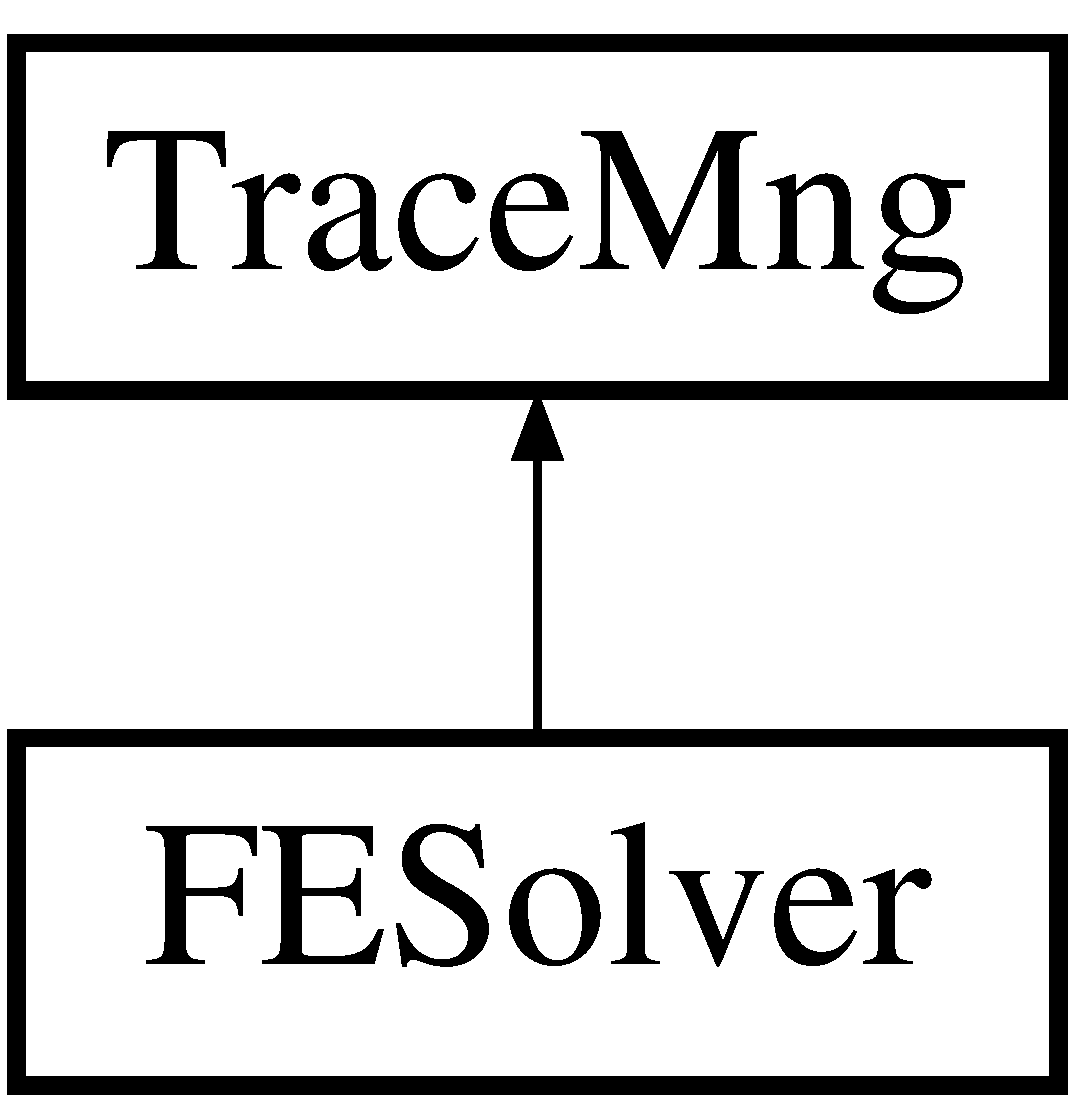
\includegraphics[height=2cm]{classFESolver}
\end{center}
\end{figure}
\subsection*{Public Member Functions}
\begin{DoxyCompactItemize}
\item 
\hypertarget{classFESolver_a131a56fa01a75f28e7bcf0dcbd5627b7}{
void {\bfseries setRHSFunction} (\hyperlink{classIRHSFunction}{IRHSFunction} $\ast$fun)}
\label{classFESolver_a131a56fa01a75f28e7bcf0dcbd5627b7}

\item 
\hypertarget{classFESolver_afa2236c236e3ed9b445945f6b6f9db54}{
void {\bfseries compute} ()}
\label{classFESolver_afa2236c236e3ed9b445945f6b6f9db54}

\item 
\hypertarget{classFESolver_a75187f8017010a24af1f1dc363c29660}{
void {\bfseries setInput} (\hyperlink{classFESolverInput}{FESolverInput} input)}
\label{classFESolver_a75187f8017010a24af1f1dc363c29660}

\item 
\hypertarget{classFESolver_a9841eb6057fa694d6cea2fa4300483e0}{
\hyperlink{classFESolverOutput}{FESolverOutput} {\bfseries getOutputFE} ()}
\label{classFESolver_a9841eb6057fa694d6cea2fa4300483e0}

\end{DoxyCompactItemize}


The documentation for this class was generated from the following files:\begin{DoxyCompactItemize}
\item 
FESolver/FESolver.h\item 
FESolver/FESolver.cpp\end{DoxyCompactItemize}

\hypertarget{classFESolverInput}{
\section{FESolverInput Class Reference}
\label{classFESolverInput}\index{FESolverInput@{FESolverInput}}
}
\subsection*{Public Member Functions}
\begin{DoxyCompactItemize}
\item 
\hypertarget{classFESolverInput_a88ad8d5ea0ba74e1b83e1ef7ed3350fc}{
void {\bfseries set} (Real t0, Real dt, RealVector \&y0)}
\label{classFESolverInput_a88ad8d5ea0ba74e1b83e1ef7ed3350fc}

\item 
\hypertarget{classFESolverInput_ab86ff7eea7fca1e7ad6a02848a4b34e0}{
Real {\bfseries getDt} () const }
\label{classFESolverInput_ab86ff7eea7fca1e7ad6a02848a4b34e0}

\item 
\hypertarget{classFESolverInput_a0c71112b0a658da15e04ec636cc31acc}{
Real {\bfseries getT0} () const }
\label{classFESolverInput_a0c71112b0a658da15e04ec636cc31acc}

\item 
\hypertarget{classFESolverInput_aa5765164c5aa548129d84cd1bf3446d7}{
const RealVector \& {\bfseries getY0} () const }
\label{classFESolverInput_aa5765164c5aa548129d84cd1bf3446d7}

\end{DoxyCompactItemize}


The documentation for this class was generated from the following files:\begin{DoxyCompactItemize}
\item 
FESolver/FESolverInput.h\item 
FESolver/FESolverInput.cpp\end{DoxyCompactItemize}

\hypertarget{classFESolverOutput}{
\section{FESolverOutput Class Reference}
\label{classFESolverOutput}\index{FESolverOutput@{FESolverOutput}}
}
\subsection*{Public Member Functions}
\begin{DoxyCompactItemize}
\item 
\hypertarget{classFESolverOutput_a890577c0649e10516ef34c9fc027d058}{
void {\bfseries setYFinal} (const RealVector \&final)}
\label{classFESolverOutput_a890577c0649e10516ef34c9fc027d058}

\item 
\hypertarget{classFESolverOutput_addc33a0512e2e53c6f9b3a845b9759a5}{
const RealVector \& {\bfseries getYFinal} () const }
\label{classFESolverOutput_addc33a0512e2e53c6f9b3a845b9759a5}

\item 
\hypertarget{classFESolverOutput_a0648c1129ea238be4b20889e2b1726cb}{
Real {\bfseries getTFinal} () const }
\label{classFESolverOutput_a0648c1129ea238be4b20889e2b1726cb}

\item 
\hypertarget{classFESolverOutput_a1e060bdb866aa2f89d62f5e191b39c32}{
Bool {\bfseries getIsConverged} () const }
\label{classFESolverOutput_a1e060bdb866aa2f89d62f5e191b39c32}

\item 
\hypertarget{classFESolverOutput_ab1edc441da120ef956fcfd647352e0e2}{
void {\bfseries setIsConverged} (Bool isConverged)}
\label{classFESolverOutput_ab1edc441da120ef956fcfd647352e0e2}

\item 
\hypertarget{classFESolverOutput_aa4150e5690c01bf135659b8f86cbd39d}{
void {\bfseries setTFinal} (const Real final)}
\label{classFESolverOutput_aa4150e5690c01bf135659b8f86cbd39d}

\end{DoxyCompactItemize}


The documentation for this class was generated from the following files:\begin{DoxyCompactItemize}
\item 
FESolver/FESolverOutput.h\item 
FESolver/FESolverOutput.cpp\end{DoxyCompactItemize}

\hypertarget{classFESolverUtils}{
\section{FESolverUtils Class Reference}
\label{classFESolverUtils}\index{FESolverUtils@{FESolverUtils}}
}
Inheritance diagram for FESolverUtils::\begin{figure}[H]
\begin{center}
\leavevmode
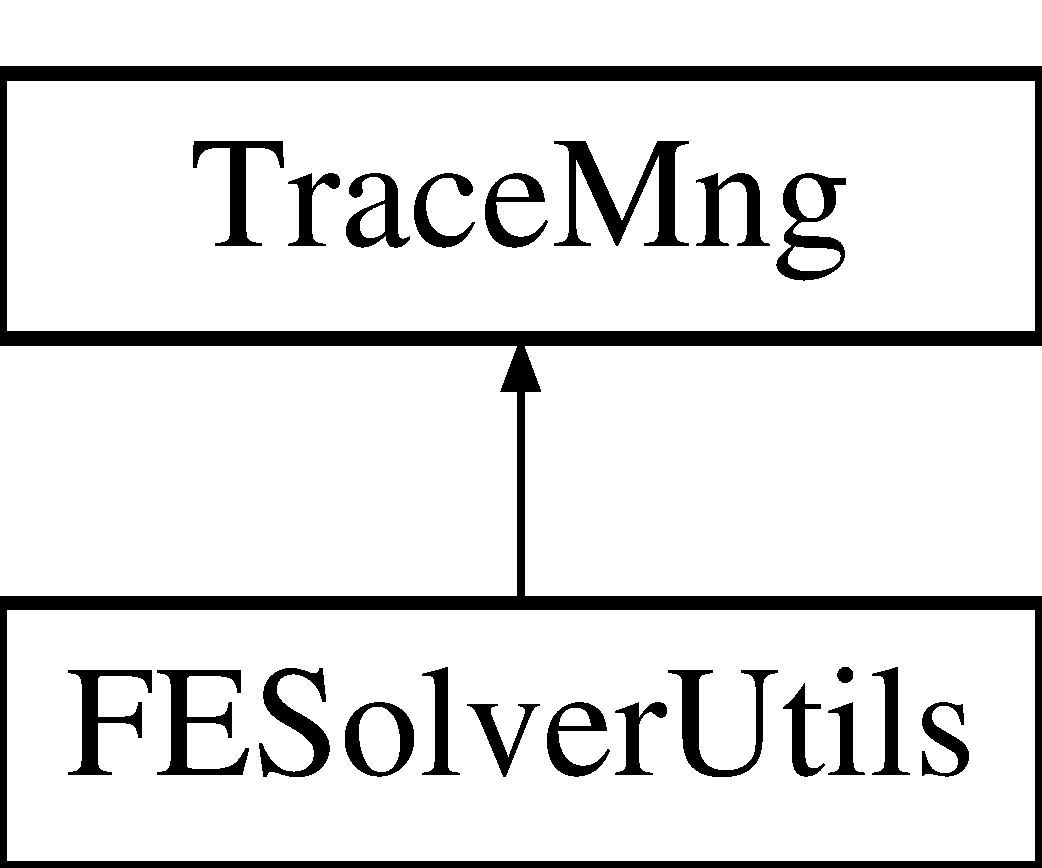
\includegraphics[height=2cm]{classFESolverUtils}
\end{center}
\end{figure}
\subsection*{Public Member Functions}
\begin{DoxyCompactItemize}
\item 
\hypertarget{classFESolverUtils_a7a97d0b724004bed7df58855607c25fe}{
void \hyperlink{classFESolverUtils_a7a97d0b724004bed7df58855607c25fe}{printInfo} (\hyperlink{classFESolverOutput}{FESolverOutput} output)}
\label{classFESolverUtils_a7a97d0b724004bed7df58855607c25fe}

\begin{DoxyCompactList}\small\item\em Outputs some info on the time step solver. \item\end{DoxyCompactList}\end{DoxyCompactItemize}


The documentation for this class was generated from the following files:\begin{DoxyCompactItemize}
\item 
FESolver/FESolverUtils.h\item 
FESolver/FESolverUtils.cpp\end{DoxyCompactItemize}

\hypertarget{classFixedJacobianNewtonSolver}{
\section{FixedJacobianNewtonSolver Class Reference}
\label{classFixedJacobianNewtonSolver}\index{FixedJacobianNewtonSolver@{FixedJacobianNewtonSolver}}
}
Inheritance diagram for FixedJacobianNewtonSolver::\begin{figure}[H]
\begin{center}
\leavevmode
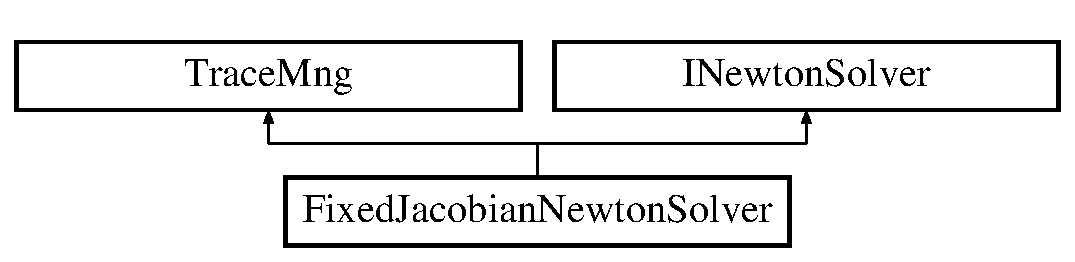
\includegraphics[height=2cm]{classFixedJacobianNewtonSolver}
\end{center}
\end{figure}
\subsection*{Public Member Functions}
\begin{DoxyCompactItemize}
\item 
void \hyperlink{classFixedJacobianNewtonSolver_a0afd96a1a9a1622f27cbe7b3fa345d01}{compute} (\hyperlink{classINewtonFunction}{INewtonFunction} \&fun, RealMatrixSparse \&J, RealVector \&Y, const Real tol\_\-rel, const Real tol\_\-abs, Bool \&diverge\_\-Newton, const Integer MaxNewtonStep)
\begin{DoxyCompactList}\small\item\em Function to compute the solution with the inexat Newton method for non linear system the Jacobian is fixed. \item\end{DoxyCompactList}\end{DoxyCompactItemize}


\subsection{Member Function Documentation}
\hypertarget{classFixedJacobianNewtonSolver_a0afd96a1a9a1622f27cbe7b3fa345d01}{
\index{FixedJacobianNewtonSolver@{FixedJacobianNewtonSolver}!compute@{compute}}
\index{compute@{compute}!FixedJacobianNewtonSolver@{FixedJacobianNewtonSolver}}
\subsubsection[{compute}]{\setlength{\rightskip}{0pt plus 5cm}void FixedJacobianNewtonSolver::compute ({\bf INewtonFunction} \& {\em fun}, \/  RealMatrixSparse \& {\em J}, \/  RealVector \& {\em Y}, \/  const Real {\em tol\_\-rel}, \/  const Real {\em tol\_\-abs}, \/  Bool \& {\em diverge\_\-Newton}, \/  const Integer {\em MaxNewtonStep})\hspace{0.3cm}{\ttfamily  \mbox{[}virtual\mbox{]}}}}
\label{classFixedJacobianNewtonSolver_a0afd96a1a9a1622f27cbe7b3fa345d01}


Function to compute the solution with the inexat Newton method for non linear system the Jacobian is fixed. Returns the solution by reference 

Implements \hyperlink{classINewtonSolver_aaf2a0a6fbf03d4f58ba24e47590458d0}{INewtonSolver}.

The documentation for this class was generated from the following files:\begin{DoxyCompactItemize}
\item 
NewtonSolver/FixedJacobianNewtonSolver.h\item 
NewtonSolver/FixedJacobianNewtonSolver.cpp\end{DoxyCompactItemize}

\hypertarget{classTraceOut_1_1Flux}{
\section{TraceOut::Flux Class Reference}
\label{classTraceOut_1_1Flux}\index{TraceOut::Flux@{TraceOut::Flux}}
}
\subsection*{Public Member Functions}
\begin{DoxyCompactItemize}
\item 
\hypertarget{classTraceOut_1_1Flux_aa39e09f5dd5bfa04a8be3eef8cfa17cd}{
{\bfseries Flux} (std::ostream \&os, bool \&is\_\-fatal)}
\label{classTraceOut_1_1Flux_aa39e09f5dd5bfa04a8be3eef8cfa17cd}

\end{DoxyCompactItemize}
\subsection*{Public Attributes}
\begin{DoxyCompactItemize}
\item 
\hypertarget{classTraceOut_1_1Flux_a4ea5098a346240d4a5d8af0b8aa5f205}{
std::ostream \& {\bfseries f\_\-os}}
\label{classTraceOut_1_1Flux_a4ea5098a346240d4a5d8af0b8aa5f205}

\item 
\hypertarget{classTraceOut_1_1Flux_a04866de0cc0e129c146e7f9d51aa0304}{
bool \& {\bfseries f\_\-is\_\-fatal}}
\label{classTraceOut_1_1Flux_a04866de0cc0e129c146e7f9d51aa0304}

\end{DoxyCompactItemize}


The documentation for this class was generated from the following file:\begin{DoxyCompactItemize}
\item 
TraceMng.h\end{DoxyCompactItemize}

\hypertarget{classGeochemistryParameters}{
\section{GeochemistryParameters Class Reference}
\label{classGeochemistryParameters}\index{GeochemistryParameters@{GeochemistryParameters}}
}


Parameters necessary to build the Geochemistry RHS Function.  


{\ttfamily \#include $<$GeochemistryParameters.h$>$}\subsection*{Public Member Functions}
\begin{DoxyCompactItemize}
\item 
\hypertarget{classGeochemistryParameters_abe67b2fbbba26c71333d8dc5fa33ea17}{
const RealVector \& {\bfseries getKReaction} () const }
\label{classGeochemistryParameters_abe67b2fbbba26c71333d8dc5fa33ea17}

\item 
\hypertarget{classGeochemistryParameters_a519272ad201baee1c117b3471b7f7a4d}{
void {\bfseries setKReaction} (const RealVector \&reactions)}
\label{classGeochemistryParameters_a519272ad201baee1c117b3471b7f7a4d}

\item 
\hypertarget{classGeochemistryParameters_a8ed20d1f41db8f3c651e7ae9179e42a1}{
const RealVector \& {\bfseries getLogK} () const }
\label{classGeochemistryParameters_a8ed20d1f41db8f3c651e7ae9179e42a1}

\item 
\hypertarget{classGeochemistryParameters_a6cf912426641b20ca80f72d3b6d5c5d4}{
void {\bfseries setLogK} (const RealVector \&logK)}
\label{classGeochemistryParameters_a6cf912426641b20ca80f72d3b6d5c5d4}

\item 
\hypertarget{classGeochemistryParameters_aaf7f26a4a54c58f8a9b5d0f9e44226a3}{
const StringVector \& {\bfseries getPhase} () const }
\label{classGeochemistryParameters_aaf7f26a4a54c58f8a9b5d0f9e44226a3}

\item 
\hypertarget{classGeochemistryParameters_a2e1b7c736879949560195d02754fe466}{
void {\bfseries setPhase} (const StringVector \&phase)}
\label{classGeochemistryParameters_a2e1b7c736879949560195d02754fe466}

\item 
\hypertarget{classGeochemistryParameters_a05ba8a6df36d04cc63f2faa313d3b4c7}{
const StringVector \& {\bfseries getPhaseLaw} () const }
\label{classGeochemistryParameters_a05ba8a6df36d04cc63f2faa313d3b4c7}

\item 
\hypertarget{classGeochemistryParameters_affd3051edc17f64242ab7eb3a476bb75}{
void {\bfseries setPhaseLaw} (const StringVector \&phaseLaw)}
\label{classGeochemistryParameters_affd3051edc17f64242ab7eb3a476bb75}

\item 
\hypertarget{classGeochemistryParameters_aff2a5716e26bf445c2ef41f76a9f8529}{
const StringVector \& {\bfseries getPhaseModel} () const }
\label{classGeochemistryParameters_aff2a5716e26bf445c2ef41f76a9f8529}

\item 
\hypertarget{classGeochemistryParameters_a3138434a1b35ca7a1ec3ab2f5584c59a}{
void {\bfseries setPhaseModel} (const StringVector \&phaseModel)}
\label{classGeochemistryParameters_a3138434a1b35ca7a1ec3ab2f5584c59a}

\item 
\hypertarget{classGeochemistryParameters_ae3b075ec3d81e2769cad8eb80c5c2970}{
const StringVector \& {\bfseries getReaction} () const }
\label{classGeochemistryParameters_ae3b075ec3d81e2769cad8eb80c5c2970}

\item 
\hypertarget{classGeochemistryParameters_a3a53b3df20f8cc51eebec809bc61bc23}{
void {\bfseries setReaction} (const StringVector \&reaction)}
\label{classGeochemistryParameters_a3a53b3df20f8cc51eebec809bc61bc23}

\item 
\hypertarget{classGeochemistryParameters_af788c888d3687a7b3cb2d781eb3223c4}{
const RealMatrixSparse \& {\bfseries getMatrix} () const }
\label{classGeochemistryParameters_af788c888d3687a7b3cb2d781eb3223c4}

\item 
\hypertarget{classGeochemistryParameters_aa1b7ae943f93cc695a9efe3bf31d80c1}{
void {\bfseries setMatrix} (const RealMatrixSparse \&matrix)}
\label{classGeochemistryParameters_aa1b7ae943f93cc695a9efe3bf31d80c1}

\item 
\hypertarget{classGeochemistryParameters_a72f9fdd76ad845d43f224c321d46592e}{
const StringVector \& {\bfseries getSModel} () const }
\label{classGeochemistryParameters_a72f9fdd76ad845d43f224c321d46592e}

\item 
\hypertarget{classGeochemistryParameters_a5598f30c8860f910b30e37824ec63a23}{
void {\bfseries setSModel} (const StringVector \&model)}
\label{classGeochemistryParameters_a5598f30c8860f910b30e37824ec63a23}

\item 
\hypertarget{classGeochemistryParameters_afe5e999d8db3f175bfe233e34dc8e621}{
const StringVector \& {\bfseries getSpecies} () const }
\label{classGeochemistryParameters_afe5e999d8db3f175bfe233e34dc8e621}

\item 
\hypertarget{classGeochemistryParameters_a884ca7ffb7b3f80f7db0e995ac9c83b9}{
void {\bfseries setSpecies} (const StringVector \&species)}
\label{classGeochemistryParameters_a884ca7ffb7b3f80f7db0e995ac9c83b9}

\item 
\hypertarget{classGeochemistryParameters_a2795fdf359649341c45e86d6c7ea3831}{
const StringVector \& {\bfseries getSpeciesModel} () const }
\label{classGeochemistryParameters_a2795fdf359649341c45e86d6c7ea3831}

\item 
\hypertarget{classGeochemistryParameters_a9df2e901f16047ad6b079601b9d059ba}{
void {\bfseries setSpeciesModel} (const StringVector \&speciesModel)}
\label{classGeochemistryParameters_a9df2e901f16047ad6b079601b9d059ba}

\item 
\hypertarget{classGeochemistryParameters_a48646a5c66d883471803c3bcf8dce9fd}{
const StringVector \& {\bfseries getSpeciesPhase} () const }
\label{classGeochemistryParameters_a48646a5c66d883471803c3bcf8dce9fd}

\item 
\hypertarget{classGeochemistryParameters_a64597072499d818de8eb9d7cde120c46}{
void {\bfseries setSpeciesPhase} (const StringVector \&speciesPhase)}
\label{classGeochemistryParameters_a64597072499d818de8eb9d7cde120c46}

\item 
\hypertarget{classGeochemistryParameters_ab36064d9dbddb0d925dd4726079acb22}{
const RealVector \& {\bfseries getScostant} () const }
\label{classGeochemistryParameters_ab36064d9dbddb0d925dd4726079acb22}

\item 
\hypertarget{classGeochemistryParameters_a58c5c789c15a470822b98adc8c08012c}{
void {\bfseries setScostant} (const RealVector \&scostant)}
\label{classGeochemistryParameters_a58c5c789c15a470822b98adc8c08012c}

\end{DoxyCompactItemize}


\subsection{Detailed Description}
Parameters necessary to build the Geochemistry RHS Function. 

The documentation for this class was generated from the following files:\begin{DoxyCompactItemize}
\item 
GeochemistryRHSFunction/GeochemistryParameters.h\item 
GeochemistryRHSFunction/GeochemistryParameters.cpp\end{DoxyCompactItemize}

\hypertarget{classGeochemistryRHSFunction}{
\section{GeochemistryRHSFunction Class Reference}
\label{classGeochemistryRHSFunction}\index{GeochemistryRHSFunction@{GeochemistryRHSFunction}}
}


Geochemistry function.  


{\ttfamily \#include $<$GeochemistryRHSFunction.h$>$}Inheritance diagram for GeochemistryRHSFunction::\begin{figure}[H]
\begin{center}
\leavevmode
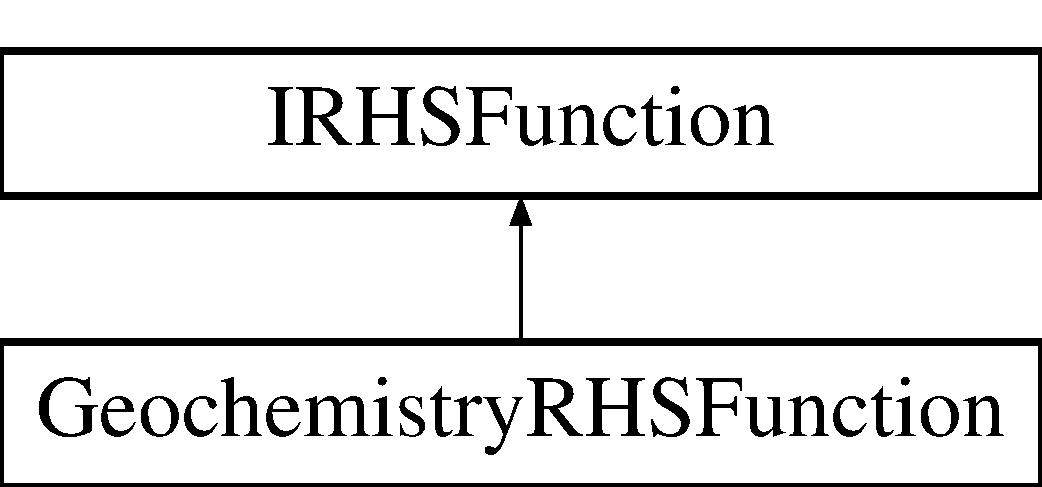
\includegraphics[height=2cm]{classGeochemistryRHSFunction}
\end{center}
\end{figure}
\subsection*{Public Member Functions}
\begin{DoxyCompactItemize}
\item 
\hypertarget{classGeochemistryRHSFunction_ab2a3ed2ba939f826922a540bfea66170}{
const \hyperlink{classGeochemistryParameters}{GeochemistryParameters} \& {\bfseries getParameters} () const }
\label{classGeochemistryRHSFunction_ab2a3ed2ba939f826922a540bfea66170}

\item 
\hypertarget{classGeochemistryRHSFunction_ad13a354a864092c722abdf5a28daa5f6}{
void {\bfseries setParameters} (const \hyperlink{classGeochemistryParameters}{GeochemistryParameters} \&parameters)}
\label{classGeochemistryRHSFunction_ad13a354a864092c722abdf5a28daa5f6}

\item 
RealVector \hyperlink{classGeochemistryRHSFunction_a2f7125c7c0ae977aea796acc9ea63e82}{evalF} (Real time, RealVector \&y)
\begin{DoxyCompactList}\small\item\em Returns a vector that it is the RHS evaluated at a certain time and solution. \item\end{DoxyCompactList}\item 
RealVector \hyperlink{classGeochemistryRHSFunction_a55eef411737aff551702c1a56d9673a1}{evalF} (Real time, RealVector \&y, IntegerVector \&ref)
\begin{DoxyCompactList}\small\item\em Returns a vector that it is the RHS evaluated at a certain time and solution only for the active components. \item\end{DoxyCompactList}\item 
RealMatrixSparse \hyperlink{classGeochemistryRHSFunction_a851506d3afa8a261a69e88421239b5e8}{evaldFdY} (Real time, RealVector \&y)
\begin{DoxyCompactList}\small\item\em Returns the Jacobian matrix at a certain time and solution. \item\end{DoxyCompactList}\item 
RealMatrixSparse \hyperlink{classGeochemistryRHSFunction_a87772d1a56b1bfe204b899dc14c44ad1}{evaldFdY} (Real time, RealVector \&y, IntegerVector \&ref)
\begin{DoxyCompactList}\small\item\em Returns the Jacobian matrix at a certain time and solution only for the active components. \item\end{DoxyCompactList}\end{DoxyCompactItemize}


\subsection{Detailed Description}
Geochemistry function. 

\subsection{Member Function Documentation}
\hypertarget{classGeochemistryRHSFunction_a87772d1a56b1bfe204b899dc14c44ad1}{
\index{GeochemistryRHSFunction@{GeochemistryRHSFunction}!evaldFdY@{evaldFdY}}
\index{evaldFdY@{evaldFdY}!GeochemistryRHSFunction@{GeochemistryRHSFunction}}
\subsubsection[{evaldFdY}]{\setlength{\rightskip}{0pt plus 5cm}RealMatrixSparse GeochemistryRHSFunction::evaldFdY (Real {\em time}, \/  RealVector \& {\em y}, \/  IntegerVector \& {\em ref})\hspace{0.3cm}{\ttfamily  \mbox{[}virtual\mbox{]}}}}
\label{classGeochemistryRHSFunction_a87772d1a56b1bfe204b899dc14c44ad1}


Returns the Jacobian matrix at a certain time and solution only for the active components. It can be the analytical one or compute with finite difference, it depends by the implementation. 

this is not the exact Jacobian!

Implements \hyperlink{classIRHSFunction}{IRHSFunction}.\hypertarget{classGeochemistryRHSFunction_a851506d3afa8a261a69e88421239b5e8}{
\index{GeochemistryRHSFunction@{GeochemistryRHSFunction}!evaldFdY@{evaldFdY}}
\index{evaldFdY@{evaldFdY}!GeochemistryRHSFunction@{GeochemistryRHSFunction}}
\subsubsection[{evaldFdY}]{\setlength{\rightskip}{0pt plus 5cm}RealMatrixSparse GeochemistryRHSFunction::evaldFdY (Real {\em time}, \/  RealVector \& {\em y})\hspace{0.3cm}{\ttfamily  \mbox{[}virtual\mbox{]}}}}
\label{classGeochemistryRHSFunction_a851506d3afa8a261a69e88421239b5e8}


Returns the Jacobian matrix at a certain time and solution. It can be the analytical one or compute with finite difference, it depends by the implementation. 

this is not the exact Jacobian!

Implements \hyperlink{classIRHSFunction}{IRHSFunction}.\hypertarget{classGeochemistryRHSFunction_a55eef411737aff551702c1a56d9673a1}{
\index{GeochemistryRHSFunction@{GeochemistryRHSFunction}!evalF@{evalF}}
\index{evalF@{evalF}!GeochemistryRHSFunction@{GeochemistryRHSFunction}}
\subsubsection[{evalF}]{\setlength{\rightskip}{0pt plus 5cm}RealVector GeochemistryRHSFunction::evalF (Real {\em time}, \/  RealVector \& {\em y}, \/  IntegerVector \& {\em ref})\hspace{0.3cm}{\ttfamily  \mbox{[}virtual\mbox{]}}}}
\label{classGeochemistryRHSFunction_a55eef411737aff551702c1a56d9673a1}


Returns a vector that it is the RHS evaluated at a certain time and solution only for the active components. 

ACTIVITY PARAMETER

Reaction Thermodynamics

Kinetic Reaction

Reactive Chemistry Problem ///////////////////////////////////// 

Implements \hyperlink{classIRHSFunction}{IRHSFunction}.\hypertarget{classGeochemistryRHSFunction_a2f7125c7c0ae977aea796acc9ea63e82}{
\index{GeochemistryRHSFunction@{GeochemistryRHSFunction}!evalF@{evalF}}
\index{evalF@{evalF}!GeochemistryRHSFunction@{GeochemistryRHSFunction}}
\subsubsection[{evalF}]{\setlength{\rightskip}{0pt plus 5cm}RealVector GeochemistryRHSFunction::evalF (Real {\em time}, \/  RealVector \& {\em y})\hspace{0.3cm}{\ttfamily  \mbox{[}virtual\mbox{]}}}}
\label{classGeochemistryRHSFunction_a2f7125c7c0ae977aea796acc9ea63e82}


Returns a vector that it is the RHS evaluated at a certain time and solution. 

ACTIVITY PARAMETER

Reaction Thermodynamics

Kinetic Reaction

Reactive Chemistry Problem ///////////////////////////////////// 

Implements \hyperlink{classIRHSFunction}{IRHSFunction}.

The documentation for this class was generated from the following files:\begin{DoxyCompactItemize}
\item 
GeochemistryRHSFunction/GeochemistryRHSFunction.h\item 
GeochemistryRHSFunction/GeochemistryRHSFunction.cpp\end{DoxyCompactItemize}

\hypertarget{classGetPot}{
\section{GetPot Class Reference}
\label{classGetPot}\index{GetPot@{GetPot}}
}
\subsection*{Classes}
\begin{DoxyCompactItemize}
\item 
struct {\bfseries variable}
\end{DoxyCompactItemize}
\subsection*{Public Member Functions}
\begin{DoxyCompactItemize}
\item 
\hypertarget{classGetPot_ac36175020c34fa0b29dcadda76f6926e}{
{\bfseries GetPot} (const \hyperlink{classGetPot}{GetPot} \&)}
\label{classGetPot_ac36175020c34fa0b29dcadda76f6926e}

\item 
\hypertarget{classGetPot_a75bfaf47037a4794d02a7b48befa3ecf}{
{\bfseries GetPot} (const int argc\_\-, char $\ast$$\ast$argv\_\-, const char $\ast$FieldSeparator=0x0)}
\label{classGetPot_a75bfaf47037a4794d02a7b48befa3ecf}

\item 
\hypertarget{classGetPot_a076ce92a05d0dfe45e1982102d6b4526}{
{\bfseries GetPot} (const char $\ast$FileName, const char $\ast$CommentStart=0x0, const char $\ast$CommentEnd=0x0, const char $\ast$FieldSeparator=0x0)}
\label{classGetPot_a076ce92a05d0dfe45e1982102d6b4526}

\item 
\hypertarget{classGetPot_ac55964791c1b7ac69c8c955022539873}{
{\footnotesize template$<$typename STRING $>$ }\\{\bfseries GetPot} (const STRING \&FileName, const char $\ast$CommentStart=0x0, const char $\ast$CommentEnd=0x0, const char $\ast$FieldSeparator=0x0)}
\label{classGetPot_ac55964791c1b7ac69c8c955022539873}

\item 
\hypertarget{classGetPot_a92c9fa06ffb4b578cdbb6e9200d27249}{
\hyperlink{classGetPot}{GetPot} \& {\bfseries operator=} (const \hyperlink{classGetPot}{GetPot} \&)}
\label{classGetPot_a92c9fa06ffb4b578cdbb6e9200d27249}

\item 
\hypertarget{classGetPot_a22bb4a0e853fb40b19293f5604341a6c}{
{\bfseries GetPot} (const STRING\_\-VECTOR \&FileNameList)}
\label{classGetPot_a22bb4a0e853fb40b19293f5604341a6c}

\item 
\hypertarget{classGetPot_a57b2855086d47efa2e32cb626d1d21c9}{
void {\bfseries absorb} (const \hyperlink{classGetPot}{GetPot} \&That)}
\label{classGetPot_a57b2855086d47efa2e32cb626d1d21c9}

\item 
\hypertarget{classGetPot_acb2c8d28c7483627cc6875bf149cf8aa}{
void {\bfseries clear\_\-requests} ()}
\label{classGetPot_acb2c8d28c7483627cc6875bf149cf8aa}

\item 
\hypertarget{classGetPot_afdadd023da7b4d13ab41e15845e6bec0}{
void {\bfseries disable\_\-request\_\-recording} ()}
\label{classGetPot_afdadd023da7b4d13ab41e15845e6bec0}

\item 
\hypertarget{classGetPot_a5163b19865018750f4f3452744da2cd8}{
void {\bfseries enable\_\-request\_\-recording} ()}
\label{classGetPot_a5163b19865018750f4f3452744da2cd8}

\item 
\hypertarget{classGetPot_a4fdfa726da0722a03d9bb2fed4aab47a}{
const std::string {\bfseries operator\mbox{[}$\,$\mbox{]}} (unsigned Idx) const }
\label{classGetPot_a4fdfa726da0722a03d9bb2fed4aab47a}

\item 
\hypertarget{classGetPot_a1c017e282a0074f949ea4b6aa7bae6b6}{
int {\bfseries get} (unsigned Idx, int Default) const }
\label{classGetPot_a1c017e282a0074f949ea4b6aa7bae6b6}

\item 
\hypertarget{classGetPot_abb786eaf8984494fa8043cbd4a952407}{
double {\bfseries get} (unsigned Idx, const double \&Default) const }
\label{classGetPot_abb786eaf8984494fa8043cbd4a952407}

\item 
\hypertarget{classGetPot_a432360a5cb32d189e3364c09d41306ca}{
const std::string {\bfseries get} (unsigned Idx, const char $\ast$Default) const }
\label{classGetPot_a432360a5cb32d189e3364c09d41306ca}

\item 
\hypertarget{classGetPot_a2d932ac1adaa8c96cd7d6a9379bee729}{
unsigned {\bfseries size} () const }
\label{classGetPot_a2d932ac1adaa8c96cd7d6a9379bee729}

\item 
\hypertarget{classGetPot_ae0ca20c8e8ddd2908d8d47e0a2d0569b}{
bool {\bfseries options\_\-contain} (const char $\ast$FlagList) const }
\label{classGetPot_ae0ca20c8e8ddd2908d8d47e0a2d0569b}

\item 
\hypertarget{classGetPot_a30b6999f373de76e53eb702667b0b09f}{
bool {\bfseries argument\_\-contains} (unsigned Idx, const char $\ast$FlagList) const }
\label{classGetPot_a30b6999f373de76e53eb702667b0b09f}

\item 
\hypertarget{classGetPot_ae8ef969f90efc0b45d53265c45b4ae4d}{
bool {\bfseries operator()} (const char $\ast$VarName, bool Default) const }
\label{classGetPot_ae8ef969f90efc0b45d53265c45b4ae4d}

\item 
\hypertarget{classGetPot_a97a8b10f961e4401ef6f6db3b4642c78}{
int {\bfseries operator()} (const char $\ast$VarName, int Default) const }
\label{classGetPot_a97a8b10f961e4401ef6f6db3b4642c78}

\item 
\hypertarget{classGetPot_a9064c182ca259bead82b93d3083eb9ab}{
double {\bfseries operator()} (const char $\ast$VarName, const double \&Default) const }
\label{classGetPot_a9064c182ca259bead82b93d3083eb9ab}

\item 
\hypertarget{classGetPot_adc0c5a1666bce6eac40d24f444801d68}{
const std::string {\bfseries operator()} (const char $\ast$VarName, const char $\ast$Default) const }
\label{classGetPot_adc0c5a1666bce6eac40d24f444801d68}

\item 
\hypertarget{classGetPot_af87d43a0947c7464416434787821b59a}{
bool {\bfseries operator()} (const char $\ast$VarName, bool Default, bool \&found) const }
\label{classGetPot_af87d43a0947c7464416434787821b59a}

\item 
\hypertarget{classGetPot_a63be4fe6c4bb9fa1a08f1b36c9c60ffe}{
int {\bfseries operator()} (const char $\ast$VarName, int Default, bool \&found) const }
\label{classGetPot_a63be4fe6c4bb9fa1a08f1b36c9c60ffe}

\item 
\hypertarget{classGetPot_a526e6534609b0157a57959923f51fe93}{
double {\bfseries operator()} (const char $\ast$VarName, const double \&Default, bool \&found) const }
\label{classGetPot_a526e6534609b0157a57959923f51fe93}

\item 
\hypertarget{classGetPot_a7e54e5aa5777277a5bea8fdec05d6590}{
const std::string {\bfseries operator()} (const char $\ast$VarName, const char $\ast$Default, bool \&found) const }
\label{classGetPot_a7e54e5aa5777277a5bea8fdec05d6590}

\item 
\hypertarget{classGetPot_a17489588d77437b4e8b6d6b002a8898d}{
bool {\bfseries operator()} (const char $\ast$VarName, bool Default, unsigned Idx) const }
\label{classGetPot_a17489588d77437b4e8b6d6b002a8898d}

\item 
\hypertarget{classGetPot_a403ee188f1ba0447569cd982cb9dcc44}{
int {\bfseries operator()} (const char $\ast$VarName, int Default, unsigned Idx) const }
\label{classGetPot_a403ee188f1ba0447569cd982cb9dcc44}

\item 
\hypertarget{classGetPot_aa269bc0f2f7b3ea56b56aec8054d2f98}{
double {\bfseries operator()} (const char $\ast$VarName, const double \&Default, unsigned Idx) const }
\label{classGetPot_aa269bc0f2f7b3ea56b56aec8054d2f98}

\item 
\hypertarget{classGetPot_ad7781191cffcf56db83267ed29eb2204}{
const std::string {\bfseries operator()} (const char $\ast$VarName, const char $\ast$Default, unsigned Idx) const }
\label{classGetPot_ad7781191cffcf56db83267ed29eb2204}

\item 
\hypertarget{classGetPot_a389eb9b67c5ff84394c648932b1d717f}{
void {\bfseries set} (const char $\ast$VarName, const char $\ast$Value, const bool Requested=true)}
\label{classGetPot_a389eb9b67c5ff84394c648932b1d717f}

\item 
\hypertarget{classGetPot_a9d9386ce9c4538015b0c8b6e8fda52ee}{
void {\bfseries set} (const char $\ast$VarName, const double \&Value, const bool Requested=true)}
\label{classGetPot_a9d9386ce9c4538015b0c8b6e8fda52ee}

\item 
\hypertarget{classGetPot_a6f5c03e5370a9f4ea7216fdfcec576b1}{
void {\bfseries set} (const char $\ast$VarName, const int Value, const bool Requested=true)}
\label{classGetPot_a6f5c03e5370a9f4ea7216fdfcec576b1}

\item 
\hypertarget{classGetPot_acebb6f432d3749c950ae732eb9fa7b21}{
bool {\bfseries checkVariable} (const char $\ast$VarName) const }
\label{classGetPot_acebb6f432d3749c950ae732eb9fa7b21}

\item 
\hypertarget{classGetPot_ac58129dc7b1cccfa45a7175f33c8d6c3}{
unsigned {\bfseries vector\_\-variable\_\-size} (const char $\ast$VarName) const }
\label{classGetPot_ac58129dc7b1cccfa45a7175f33c8d6c3}

\item 
\hypertarget{classGetPot_a811c7b5230512718ec8f82de6662f28f}{
STRING\_\-VECTOR {\bfseries get\_\-variable\_\-names} () const }
\label{classGetPot_a811c7b5230512718ec8f82de6662f28f}

\item 
\hypertarget{classGetPot_a2dfc532c29426f5010cc07f2f07a5ea3}{
STRING\_\-VECTOR {\bfseries get\_\-section\_\-names} () const }
\label{classGetPot_a2dfc532c29426f5010cc07f2f07a5ea3}

\item 
\hypertarget{classGetPot_a19e24ca540e9e72ea3a8a8780d950a22}{
void {\bfseries set\_\-prefix} (const char $\ast$Prefix)}
\label{classGetPot_a19e24ca540e9e72ea3a8a8780d950a22}

\item 
\hypertarget{classGetPot_a5d6af0d1618f40cb9d0acaba79931014}{
bool {\bfseries search\_\-failed} () const }
\label{classGetPot_a5d6af0d1618f40cb9d0acaba79931014}

\item 
\hypertarget{classGetPot_a84b0e0199ae3df63c01ea125a16be83f}{
void {\bfseries disable\_\-loop} ()}
\label{classGetPot_a84b0e0199ae3df63c01ea125a16be83f}

\item 
\hypertarget{classGetPot_a99f8e9cc6ff54d0abf4ef090cd39d8a7}{
void {\bfseries enable\_\-loop} ()}
\label{classGetPot_a99f8e9cc6ff54d0abf4ef090cd39d8a7}

\item 
\hypertarget{classGetPot_ad55107a9bd39804599844194218e8e3a}{
void {\bfseries reset\_\-cursor} ()}
\label{classGetPot_ad55107a9bd39804599844194218e8e3a}

\item 
\hypertarget{classGetPot_af8d29a623cd9a37d9f133c66b712efc5}{
void {\bfseries init\_\-multiple\_\-occurrence} ()}
\label{classGetPot_af8d29a623cd9a37d9f133c66b712efc5}

\item 
\hypertarget{classGetPot_a183e68216495d2afe4fb1d3a6363718d}{
bool {\bfseries search} (const char $\ast$option)}
\label{classGetPot_a183e68216495d2afe4fb1d3a6363718d}

\item 
\hypertarget{classGetPot_aba4993d981a043ea377eed1588f6da98}{
bool {\bfseries search} (unsigned No, const char $\ast$P,...)}
\label{classGetPot_aba4993d981a043ea377eed1588f6da98}

\item 
\hypertarget{classGetPot_ab198c8915bf041f409d021d947a63c8d}{
int {\bfseries next} (int Default)}
\label{classGetPot_ab198c8915bf041f409d021d947a63c8d}

\item 
\hypertarget{classGetPot_a0c492a6a937df46a8bf7107c8960743b}{
double {\bfseries next} (const double \&Default)}
\label{classGetPot_a0c492a6a937df46a8bf7107c8960743b}

\item 
\hypertarget{classGetPot_a295a0e34f2553a5ac76ace0adcfa023f}{
const std::string {\bfseries next} (const char $\ast$Default)}
\label{classGetPot_a295a0e34f2553a5ac76ace0adcfa023f}

\item 
\hypertarget{classGetPot_aaa1c2b835b2599c5c087d2d4f82e368b}{
int {\bfseries follow} (int Default, const char $\ast$Option)}
\label{classGetPot_aaa1c2b835b2599c5c087d2d4f82e368b}

\item 
\hypertarget{classGetPot_a855b9098faff198692edae7741573065}{
double {\bfseries follow} (const double \&Default, const char $\ast$Option)}
\label{classGetPot_a855b9098faff198692edae7741573065}

\item 
\hypertarget{classGetPot_a091faf970647b60ffdbc74a27160e6b1}{
const std::string {\bfseries follow} (const char $\ast$Default, const char $\ast$Option)}
\label{classGetPot_a091faf970647b60ffdbc74a27160e6b1}

\item 
\hypertarget{classGetPot_a55bfc61743e387853e6939e7fa70b5ee}{
int {\bfseries follow} (int Default, unsigned No, const char $\ast$Option,...)}
\label{classGetPot_a55bfc61743e387853e6939e7fa70b5ee}

\item 
\hypertarget{classGetPot_af8f391bb9b55d0fd01ce1e74282d2cdf}{
double {\bfseries follow} (const double \&Default, unsigned No, const char $\ast$Option,...)}
\label{classGetPot_af8f391bb9b55d0fd01ce1e74282d2cdf}

\item 
\hypertarget{classGetPot_ad32ef7ad9fdcd024f250da838197d7a8}{
const std::string {\bfseries follow} (const char $\ast$Default, unsigned No, const char $\ast$Option,...)}
\label{classGetPot_ad32ef7ad9fdcd024f250da838197d7a8}

\item 
\hypertarget{classGetPot_ad86cc5f063845dd24f0aa9e8500317b1}{
std::vector$<$ std::string $>$ {\bfseries nominus\_\-followers} (const char $\ast$Option)}
\label{classGetPot_ad86cc5f063845dd24f0aa9e8500317b1}

\item 
\hypertarget{classGetPot_a3c0bc7200bc2558217039050b9087d97}{
std::vector$<$ std::string $>$ {\bfseries nominus\_\-followers} (unsigned No,...)}
\label{classGetPot_a3c0bc7200bc2558217039050b9087d97}

\item 
\hypertarget{classGetPot_a2eec5ed54d86646402e5e16485601fea}{
int {\bfseries direct\_\-follow} (int Default, const char $\ast$Option)}
\label{classGetPot_a2eec5ed54d86646402e5e16485601fea}

\item 
\hypertarget{classGetPot_ad64bcf7d37c78bae36ad97aaac92a86b}{
double {\bfseries direct\_\-follow} (const double \&Default, const char $\ast$Option)}
\label{classGetPot_ad64bcf7d37c78bae36ad97aaac92a86b}

\item 
\hypertarget{classGetPot_aca40e39c14f630802931cac3c2aeb524}{
const std::string {\bfseries direct\_\-follow} (const char $\ast$Default, const char $\ast$Option)}
\label{classGetPot_aca40e39c14f630802931cac3c2aeb524}

\item 
\hypertarget{classGetPot_a2f79e3c21adc9568a507eb91ce15e4d0}{
std::vector$<$ std::string $>$ {\bfseries string\_\-tails} (const char $\ast$StartString)}
\label{classGetPot_a2f79e3c21adc9568a507eb91ce15e4d0}

\item 
\hypertarget{classGetPot_a269879b326c9388c7145bad57ca5fcb1}{
std::vector$<$ int $>$ {\bfseries int\_\-tails} (const char $\ast$StartString, const int Default=1)}
\label{classGetPot_a269879b326c9388c7145bad57ca5fcb1}

\item 
\hypertarget{classGetPot_aa50b6e2ea274355c930a608079a88a1f}{
std::vector$<$ double $>$ {\bfseries double\_\-tails} (const char $\ast$StartString, const double Default=1.0)}
\label{classGetPot_aa50b6e2ea274355c930a608079a88a1f}

\item 
\hypertarget{classGetPot_a2bb3ce06e8d8d1875722480254e8fc56}{
STRING\_\-VECTOR {\bfseries nominus\_\-vector} () const }
\label{classGetPot_a2bb3ce06e8d8d1875722480254e8fc56}

\item 
\hypertarget{classGetPot_ab696e5463b8a7e1e5cbab563e406db60}{
unsigned {\bfseries nominus\_\-size} () const }
\label{classGetPot_ab696e5463b8a7e1e5cbab563e406db60}

\item 
\hypertarget{classGetPot_a99f571a68efe22003f5162e739c7b801}{
std::string {\bfseries next\_\-nominus} ()}
\label{classGetPot_a99f571a68efe22003f5162e739c7b801}

\item 
\hypertarget{classGetPot_aa5c283ed5ae3f40341df871c5cdf6588}{
STRING\_\-VECTOR {\bfseries unidentified\_\-arguments} (unsigned Number, const char $\ast$Known,...) const }
\label{classGetPot_aa5c283ed5ae3f40341df871c5cdf6588}

\item 
\hypertarget{classGetPot_a08a1a9ab9ae443888718cacf10afd06d}{
STRING\_\-VECTOR {\bfseries unidentified\_\-arguments} (const STRING\_\-VECTOR \&Knowns) const }
\label{classGetPot_a08a1a9ab9ae443888718cacf10afd06d}

\item 
\hypertarget{classGetPot_a88e7f9c789b8bea223127dbfecea5041}{
STRING\_\-VECTOR {\bfseries unidentified\_\-arguments} () const }
\label{classGetPot_a88e7f9c789b8bea223127dbfecea5041}

\item 
\hypertarget{classGetPot_ac11b52993315a910ad7ee9fd5729605a}{
STRING\_\-VECTOR {\bfseries unidentified\_\-options} (unsigned Number, const char $\ast$Known,...) const }
\label{classGetPot_ac11b52993315a910ad7ee9fd5729605a}

\item 
\hypertarget{classGetPot_a70b0e051abb2af10b5bef708db80f774}{
STRING\_\-VECTOR {\bfseries unidentified\_\-options} (const STRING\_\-VECTOR \&Knowns) const }
\label{classGetPot_a70b0e051abb2af10b5bef708db80f774}

\item 
\hypertarget{classGetPot_a7a51d05e04dfdba0788c6f399120b35a}{
STRING\_\-VECTOR {\bfseries unidentified\_\-options} () const }
\label{classGetPot_a7a51d05e04dfdba0788c6f399120b35a}

\item 
\hypertarget{classGetPot_a3b4c3f3128a38c2a24c977f9c5371c1a}{
std::string {\bfseries unidentified\_\-flags} (const char $\ast$Known, int ArgumentNumber) const }
\label{classGetPot_a3b4c3f3128a38c2a24c977f9c5371c1a}

\item 
\hypertarget{classGetPot_a534677efd6bf66f2b7bbb03e2f588a7f}{
STRING\_\-VECTOR {\bfseries unidentified\_\-variables} (unsigned Number, const char $\ast$Known,...) const }
\label{classGetPot_a534677efd6bf66f2b7bbb03e2f588a7f}

\item 
\hypertarget{classGetPot_a5685c87e7392e8936fedcc74f811c504}{
STRING\_\-VECTOR {\bfseries unidentified\_\-variables} (const STRING\_\-VECTOR \&Knowns) const }
\label{classGetPot_a5685c87e7392e8936fedcc74f811c504}

\item 
\hypertarget{classGetPot_a605018ceff57881e1607608a4c978906}{
STRING\_\-VECTOR {\bfseries unidentified\_\-variables} () const }
\label{classGetPot_a605018ceff57881e1607608a4c978906}

\item 
\hypertarget{classGetPot_ada04daaaee674288521f6532ed3fbcf0}{
STRING\_\-VECTOR {\bfseries unidentified\_\-sections} (unsigned Number, const char $\ast$Known,...) const }
\label{classGetPot_ada04daaaee674288521f6532ed3fbcf0}

\item 
\hypertarget{classGetPot_a5e716f5a2db7bd7cf9ac43c1d02e16ab}{
STRING\_\-VECTOR {\bfseries unidentified\_\-sections} (const STRING\_\-VECTOR \&Knowns) const }
\label{classGetPot_a5e716f5a2db7bd7cf9ac43c1d02e16ab}

\item 
\hypertarget{classGetPot_ae54ef4d5f10fa3b5badf39e5dcda529b}{
STRING\_\-VECTOR {\bfseries unidentified\_\-sections} () const }
\label{classGetPot_ae54ef4d5f10fa3b5badf39e5dcda529b}

\item 
\hypertarget{classGetPot_a9378d42c51fe2fa8f2388c2c47744080}{
STRING\_\-VECTOR {\bfseries unidentified\_\-nominuses} (unsigned Number, const char $\ast$Known,...) const }
\label{classGetPot_a9378d42c51fe2fa8f2388c2c47744080}

\item 
\hypertarget{classGetPot_a72f3552844a9fd451cc981ca212bd74c}{
STRING\_\-VECTOR {\bfseries unidentified\_\-nominuses} (const STRING\_\-VECTOR \&Knowns) const }
\label{classGetPot_a72f3552844a9fd451cc981ca212bd74c}

\item 
\hypertarget{classGetPot_a11086beb1e3d595140617838ae16a53e}{
STRING\_\-VECTOR {\bfseries unidentified\_\-nominuses} () const }
\label{classGetPot_a11086beb1e3d595140617838ae16a53e}

\item 
\hypertarget{classGetPot_a50eb9af9aec818bf434da399bb3644d1}{
int {\bfseries print} () const }
\label{classGetPot_a50eb9af9aec818bf434da399bb3644d1}

\end{DoxyCompactItemize}


The documentation for this class was generated from the following file:\begin{DoxyCompactItemize}
\item 
GetPot.hpp\end{DoxyCompactItemize}

\hypertarget{classHyperbolicEquationRusanovFlux}{
\section{HyperbolicEquationRusanovFlux Class Reference}
\label{classHyperbolicEquationRusanovFlux}\index{HyperbolicEquationRusanovFlux@{HyperbolicEquationRusanovFlux}}
}
Inheritance diagram for HyperbolicEquationRusanovFlux::\begin{figure}[H]
\begin{center}
\leavevmode
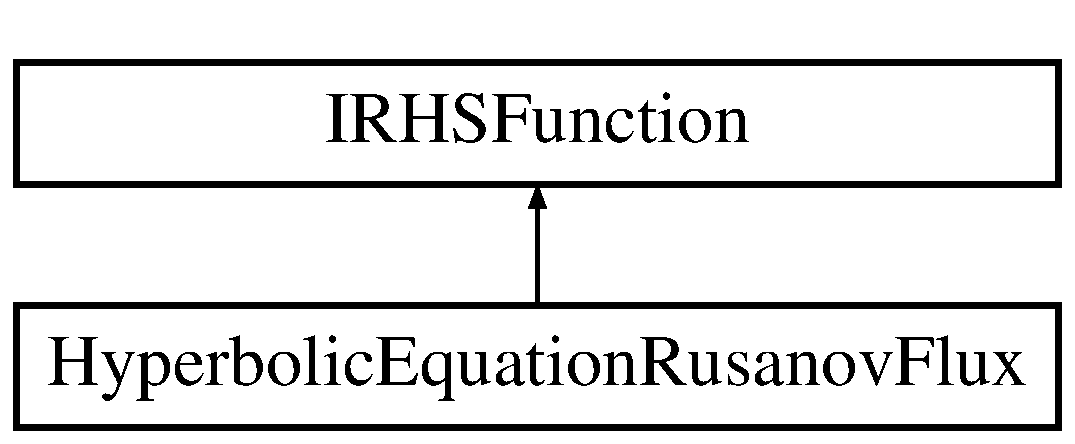
\includegraphics[height=2cm]{classHyperbolicEquationRusanovFlux}
\end{center}
\end{figure}
\subsection*{Public Member Functions}
\begin{DoxyCompactItemize}
\item 
\hypertarget{classHyperbolicEquationRusanovFlux_a38f44780041dab581b00c92f666e48be}{
Integer {\bfseries getNx} () const }
\label{classHyperbolicEquationRusanovFlux_a38f44780041dab581b00c92f666e48be}

\item 
\hypertarget{classHyperbolicEquationRusanovFlux_ab6a4dae66b856582549f1c386edd6240}{
void {\bfseries setNx} (Integer nx)}
\label{classHyperbolicEquationRusanovFlux_ab6a4dae66b856582549f1c386edd6240}

\item 
\hypertarget{classHyperbolicEquationRusanovFlux_ad29be60cc9f1554fcbb91e1c79ba15d6}{
Real {\bfseries getX0} () const }
\label{classHyperbolicEquationRusanovFlux_ad29be60cc9f1554fcbb91e1c79ba15d6}

\item 
\hypertarget{classHyperbolicEquationRusanovFlux_aedfdd231d68ffb2ed5837eab6e1f715b}{
void {\bfseries setX0} (Real x0)}
\label{classHyperbolicEquationRusanovFlux_aedfdd231d68ffb2ed5837eab6e1f715b}

\item 
\hypertarget{classHyperbolicEquationRusanovFlux_a5205073c68f3368649e1ba391b2d6346}{
Real {\bfseries getXL} () const }
\label{classHyperbolicEquationRusanovFlux_a5205073c68f3368649e1ba391b2d6346}

\item 
\hypertarget{classHyperbolicEquationRusanovFlux_a812d0ca71081816f919fc8c00cfc6500}{
void {\bfseries setXL} (Real l)}
\label{classHyperbolicEquationRusanovFlux_a812d0ca71081816f919fc8c00cfc6500}

\item 
\hypertarget{classHyperbolicEquationRusanovFlux_a702f9f6f1e607b541f877c0883fc1ca8}{
void {\bfseries setBcFunc} (\hyperlink{classIBCFunction}{IBCFunction} $\ast$bcFunc)}
\label{classHyperbolicEquationRusanovFlux_a702f9f6f1e607b541f877c0883fc1ca8}

\item 
\hypertarget{classHyperbolicEquationRusanovFlux_a165bc58a62fd625d3f2cbaeb07574efd}{
void {\bfseries setFluxFunc} (\hyperlink{classIFluxFunction}{IFluxFunction} $\ast$fl\_\-func)}
\label{classHyperbolicEquationRusanovFlux_a165bc58a62fd625d3f2cbaeb07574efd}

\item 
RealVector \hyperlink{classHyperbolicEquationRusanovFlux_a32c91624ae05d626535a45b12776ef9b}{evalF} (Real time, RealVector \&y)
\begin{DoxyCompactList}\small\item\em Returns a vector that it is the RHS evaluated at a certain time and solution. \item\end{DoxyCompactList}\item 
RealVector \hyperlink{classHyperbolicEquationRusanovFlux_ad7ae556cb8b48064d77163d554d83396}{evalF} (Real time, RealVector \&y, IntegerVector \&ref)
\begin{DoxyCompactList}\small\item\em Returns a vector that it is the RHS evaluated at a certain time and solution only for the active components. \item\end{DoxyCompactList}\item 
RealMatrixSparse \hyperlink{classHyperbolicEquationRusanovFlux_a401392a4b37dd6ec8a15817f37936d1b}{evaldFdY} (Real time, RealVector \&y)
\begin{DoxyCompactList}\small\item\em Returns the Jacobian matrix at a certain time and solution. \item\end{DoxyCompactList}\item 
RealMatrixSparse \hyperlink{classHyperbolicEquationRusanovFlux_a5bdb9a2cdb9acfffb191c77db1dc10e8}{evaldFdY} (Real time, RealVector \&y, IntegerVector \&ref)
\begin{DoxyCompactList}\small\item\em Returns the Jacobian matrix at a certain time and solution only for the active components. \item\end{DoxyCompactList}\end{DoxyCompactItemize}


\subsection{Member Function Documentation}
\hypertarget{classHyperbolicEquationRusanovFlux_a5bdb9a2cdb9acfffb191c77db1dc10e8}{
\index{HyperbolicEquationRusanovFlux@{HyperbolicEquationRusanovFlux}!evaldFdY@{evaldFdY}}
\index{evaldFdY@{evaldFdY}!HyperbolicEquationRusanovFlux@{HyperbolicEquationRusanovFlux}}
\subsubsection[{evaldFdY}]{\setlength{\rightskip}{0pt plus 5cm}RealMatrixSparse HyperbolicEquationRusanovFlux::evaldFdY (Real {\em time}, \/  RealVector \& {\em y}, \/  IntegerVector \& {\em ref})\hspace{0.3cm}{\ttfamily  \mbox{[}virtual\mbox{]}}}}
\label{classHyperbolicEquationRusanovFlux_a5bdb9a2cdb9acfffb191c77db1dc10e8}


Returns the Jacobian matrix at a certain time and solution only for the active components. It can be the analytical one or compute with finite difference, it depends by the implementation. 

this is not the exact Jacobian!

Implements \hyperlink{classIRHSFunction}{IRHSFunction}.\hypertarget{classHyperbolicEquationRusanovFlux_a401392a4b37dd6ec8a15817f37936d1b}{
\index{HyperbolicEquationRusanovFlux@{HyperbolicEquationRusanovFlux}!evaldFdY@{evaldFdY}}
\index{evaldFdY@{evaldFdY}!HyperbolicEquationRusanovFlux@{HyperbolicEquationRusanovFlux}}
\subsubsection[{evaldFdY}]{\setlength{\rightskip}{0pt plus 5cm}RealMatrixSparse HyperbolicEquationRusanovFlux::evaldFdY (Real {\em time}, \/  RealVector \& {\em y})\hspace{0.3cm}{\ttfamily  \mbox{[}virtual\mbox{]}}}}
\label{classHyperbolicEquationRusanovFlux_a401392a4b37dd6ec8a15817f37936d1b}


Returns the Jacobian matrix at a certain time and solution. It can be the analytical one or compute with finite difference, it depends by the implementation. 

this is not the exact Jacobian!

Implements \hyperlink{classIRHSFunction}{IRHSFunction}.\hypertarget{classHyperbolicEquationRusanovFlux_ad7ae556cb8b48064d77163d554d83396}{
\index{HyperbolicEquationRusanovFlux@{HyperbolicEquationRusanovFlux}!evalF@{evalF}}
\index{evalF@{evalF}!HyperbolicEquationRusanovFlux@{HyperbolicEquationRusanovFlux}}
\subsubsection[{evalF}]{\setlength{\rightskip}{0pt plus 5cm}RealVector HyperbolicEquationRusanovFlux::evalF (Real {\em time}, \/  RealVector \& {\em y}, \/  IntegerVector \& {\em ref})\hspace{0.3cm}{\ttfamily  \mbox{[}virtual\mbox{]}}}}
\label{classHyperbolicEquationRusanovFlux_ad7ae556cb8b48064d77163d554d83396}


Returns a vector that it is the RHS evaluated at a certain time and solution only for the active components. 

We use a finite volume method with Rusanov flux 

Implements \hyperlink{classIRHSFunction}{IRHSFunction}.\hypertarget{classHyperbolicEquationRusanovFlux_a32c91624ae05d626535a45b12776ef9b}{
\index{HyperbolicEquationRusanovFlux@{HyperbolicEquationRusanovFlux}!evalF@{evalF}}
\index{evalF@{evalF}!HyperbolicEquationRusanovFlux@{HyperbolicEquationRusanovFlux}}
\subsubsection[{evalF}]{\setlength{\rightskip}{0pt plus 5cm}RealVector HyperbolicEquationRusanovFlux::evalF (Real {\em time}, \/  RealVector \& {\em y})\hspace{0.3cm}{\ttfamily  \mbox{[}virtual\mbox{]}}}}
\label{classHyperbolicEquationRusanovFlux_a32c91624ae05d626535a45b12776ef9b}


Returns a vector that it is the RHS evaluated at a certain time and solution. 

I use a uniform space grid

For the first node we impose that the value is equal to the BC value.

We use a finite volume method with Rusanov flux 

Implements \hyperlink{classIRHSFunction}{IRHSFunction}.

The documentation for this class was generated from the following files:\begin{DoxyCompactItemize}
\item 
HyperbolicEquationRusanovFlux/HyperbolicEquationRusanovFlux.h\item 
HyperbolicEquationRusanovFlux/HyperbolicEquationRusanovFlux.cpp\end{DoxyCompactItemize}

\hypertarget{classIBCFunction}{
\section{IBCFunction Class Reference}
\label{classIBCFunction}\index{IBCFunction@{IBCFunction}}
}
Inheritance diagram for IBCFunction::\begin{figure}[H]
\begin{center}
\leavevmode
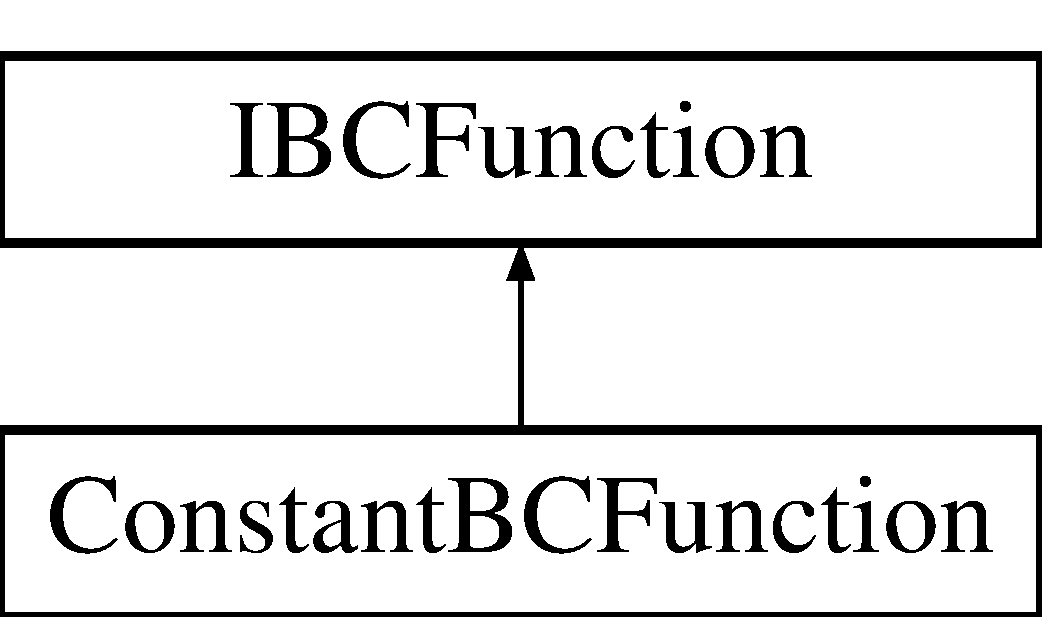
\includegraphics[height=2cm]{classIBCFunction}
\end{center}
\end{figure}
\subsection*{Public Member Functions}
\begin{DoxyCompactItemize}
\item 
\hypertarget{classIBCFunction_af301369c2049187e033bf74c0acf487c}{
virtual Real {\bfseries getValue} (Real time)=0}
\label{classIBCFunction_af301369c2049187e033bf74c0acf487c}

\end{DoxyCompactItemize}


The documentation for this class was generated from the following file:\begin{DoxyCompactItemize}
\item 
IBCFunction.h\end{DoxyCompactItemize}

\hypertarget{classIFluxFunction}{
\section{IFluxFunction Class Reference}
\label{classIFluxFunction}\index{IFluxFunction@{IFluxFunction}}
}
Inheritance diagram for IFluxFunction::\begin{figure}[H]
\begin{center}
\leavevmode
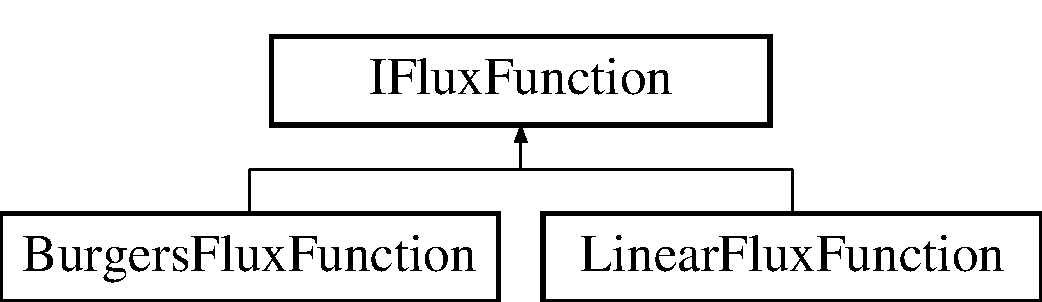
\includegraphics[height=2cm]{classIFluxFunction}
\end{center}
\end{figure}
\subsection*{Public Member Functions}
\begin{DoxyCompactItemize}
\item 
\hypertarget{classIFluxFunction_af3a7d185cf7c2d5e834b8f6872ba2110}{
virtual Real {\bfseries evalF} (Real time, Real y\_\-sol)=0}
\label{classIFluxFunction_af3a7d185cf7c2d5e834b8f6872ba2110}

\item 
\hypertarget{classIFluxFunction_a8747b84cf6abe453ca4ce7871c16275a}{
virtual Real {\bfseries evalFderivative} (Real time, Real y\_\-sol)=0}
\label{classIFluxFunction_a8747b84cf6abe453ca4ce7871c16275a}

\end{DoxyCompactItemize}


The documentation for this class was generated from the following file:\begin{DoxyCompactItemize}
\item 
IFluxFunction.h\end{DoxyCompactItemize}

\hypertarget{classIMasterSolver}{
\section{IMasterSolver Class Reference}
\label{classIMasterSolver}\index{IMasterSolver@{IMasterSolver}}
}
Inheritance diagram for IMasterSolver::\begin{figure}[H]
\begin{center}
\leavevmode
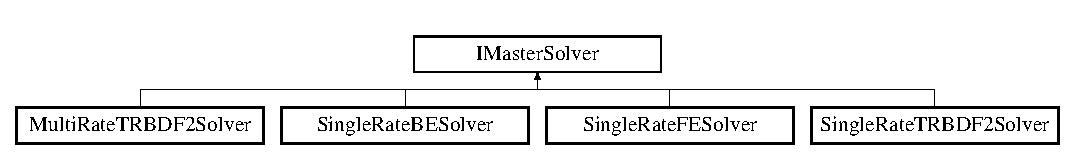
\includegraphics[height=1.70732cm]{classIMasterSolver}
\end{center}
\end{figure}
\subsection*{Public Member Functions}
\begin{DoxyCompactItemize}
\item 
\hypertarget{classIMasterSolver_a31793bc357725f331eea95a41787f0fb}{
virtual void {\bfseries setNewtSolv} (std::unique\_\-ptr$<$ \hyperlink{classINewtonSolver}{INewtonSolver} $>$ newtSolv)=0}
\label{classIMasterSolver_a31793bc357725f331eea95a41787f0fb}

\item 
\hypertarget{classIMasterSolver_a5e34f08940e8202379547f254371f9c0}{
virtual void {\bfseries setHinitial} (Real hinitial)=0}
\label{classIMasterSolver_a5e34f08940e8202379547f254371f9c0}

\item 
\hypertarget{classIMasterSolver_a7b9bf11ed562216986cf8da7a207fddf}{
virtual void {\bfseries setHz1initial} (const RealVector \&hz1initial)=0}
\label{classIMasterSolver_a7b9bf11ed562216986cf8da7a207fddf}

\item 
\hypertarget{classIMasterSolver_a0eab70f9ad2096c997a7da106a848034}{
virtual void {\bfseries setTfinal} (Real tfinal)=0}
\label{classIMasterSolver_a0eab70f9ad2096c997a7da106a848034}

\item 
\hypertarget{classIMasterSolver_a736551977fa76530ca54cc6d784cf24b}{
virtual void {\bfseries setTinitial} (Real tinitial)=0}
\label{classIMasterSolver_a736551977fa76530ca54cc6d784cf24b}

\item 
\hypertarget{classIMasterSolver_a8c9057fbaad0cb899c0b8af5cef8484f}{
virtual void {\bfseries setYinitial} (const RealVector \&yinitial)=0}
\label{classIMasterSolver_a8c9057fbaad0cb899c0b8af5cef8484f}

\item 
\hypertarget{classIMasterSolver_ad2001f3949d56db06d9756f4cc8220f5}{
virtual void {\bfseries setNewtonTolAbs} (Real newtonTolAbs)=0}
\label{classIMasterSolver_ad2001f3949d56db06d9756f4cc8220f5}

\item 
\hypertarget{classIMasterSolver_aa8142f0b762d7117a124b39d2c559036}{
virtual void {\bfseries setNewtonTolRel} (Real newtonTolRel)=0}
\label{classIMasterSolver_aa8142f0b762d7117a124b39d2c559036}

\item 
\hypertarget{classIMasterSolver_a0f4e92764161d30782c07accef08cc2e}{
virtual void {\bfseries setErrorTolAbs} (Real errorTolAbs)=0}
\label{classIMasterSolver_a0f4e92764161d30782c07accef08cc2e}

\item 
\hypertarget{classIMasterSolver_ace3b6564185972f0f1f22471c8be2faa}{
virtual void {\bfseries setErrorTolRel} (Real errorTolRel)=0}
\label{classIMasterSolver_ace3b6564185972f0f1f22471c8be2faa}

\item 
\hypertarget{classIMasterSolver_a69c6587bf3ec8d1c58a597f6138b7565}{
virtual void {\bfseries compute} ()=0}
\label{classIMasterSolver_a69c6587bf3ec8d1c58a597f6138b7565}

\item 
\hypertarget{classIMasterSolver_a23c8ea4a7018bd4daea1e911fa851715}{
virtual void {\bfseries setFun} (\hyperlink{classIRHSFunction}{IRHSFunction} $\ast$fun)=0}
\label{classIMasterSolver_a23c8ea4a7018bd4daea1e911fa851715}

\item 
\hypertarget{classIMasterSolver_a19e1fb93fa07956cbe21ef24aeb23f0b}{
virtual std::vector$<$ std::unique\_\-ptr$<$ \hyperlink{classISolverData}{ISolverData} $>$ $>$ \&\& {\bfseries getSolution} ()=0}
\label{classIMasterSolver_a19e1fb93fa07956cbe21ef24aeb23f0b}

\end{DoxyCompactItemize}


The documentation for this class was generated from the following file:\begin{DoxyCompactItemize}
\item 
IMasterSolver.h\end{DoxyCompactItemize}

\hypertarget{classRestab_1_1IndexDescription}{
\section{Restab::IndexDescription Class Reference}
\label{classRestab_1_1IndexDescription}\index{Restab::IndexDescription@{Restab::IndexDescription}}
}
\subsection*{Public Member Functions}
\begin{DoxyCompactItemize}
\item 
\hypertarget{classRestab_1_1IndexDescription_a32286b1e431f828502998eb7f7e5c718}{
{\bfseries IndexDescription} (String \_\-label, String \_\-name)}
\label{classRestab_1_1IndexDescription_a32286b1e431f828502998eb7f7e5c718}

\end{DoxyCompactItemize}
\subsection*{Public Attributes}
\begin{DoxyCompactItemize}
\item 
\hypertarget{classRestab_1_1IndexDescription_a60b99f5b5a2549229060ded6574891c0}{
String {\bfseries label}}
\label{classRestab_1_1IndexDescription_a60b99f5b5a2549229060ded6574891c0}

\item 
\hypertarget{classRestab_1_1IndexDescription_a29135a01a17adeb1a09b07a613ed9507}{
String {\bfseries name}}
\label{classRestab_1_1IndexDescription_a29135a01a17adeb1a09b07a613ed9507}

\end{DoxyCompactItemize}


The documentation for this class was generated from the following file:\begin{DoxyCompactItemize}
\item 
Restab.h\end{DoxyCompactItemize}

\hypertarget{classINewtonFunction}{
\section{INewtonFunction Class Reference}
\label{classINewtonFunction}\index{INewtonFunction@{INewtonFunction}}
}
Inheritance diagram for INewtonFunction::\begin{figure}[H]
\begin{center}
\leavevmode
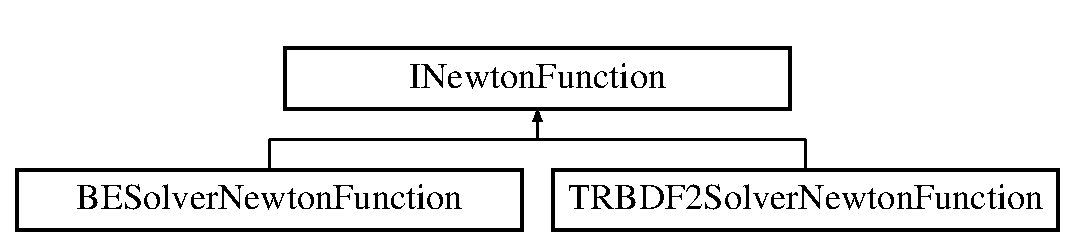
\includegraphics[height=2cm]{classINewtonFunction}
\end{center}
\end{figure}
\subsection*{Public Member Functions}
\begin{DoxyCompactItemize}
\item 
\hypertarget{classINewtonFunction_a26ac6ae8e59e3b7ceef68e80a8f688fa}{
virtual void {\bfseries evalFJ} (RealVector \&Y, RealVector \&F, RealMatrixSparse \&J)=0}
\label{classINewtonFunction_a26ac6ae8e59e3b7ceef68e80a8f688fa}

\item 
\hypertarget{classINewtonFunction_a2e0e667ea7ea91747554e6da128a246e}{
virtual void {\bfseries evalF} (RealVector \&Y, RealVector \&F)=0}
\label{classINewtonFunction_a2e0e667ea7ea91747554e6da128a246e}

\end{DoxyCompactItemize}


The documentation for this class was generated from the following file:\begin{DoxyCompactItemize}
\item 
INewtonFunction.h\end{DoxyCompactItemize}

\hypertarget{classINewtonSolver}{
\section{INewtonSolver Class Reference}
\label{classINewtonSolver}\index{INewtonSolver@{INewtonSolver}}
}
Inheritance diagram for INewtonSolver::\begin{figure}[H]
\begin{center}
\leavevmode
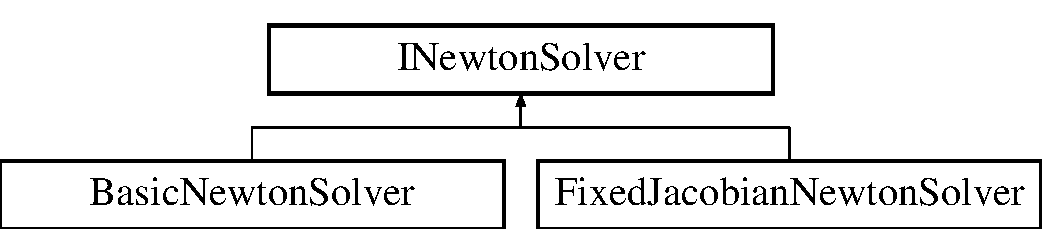
\includegraphics[height=2cm]{classINewtonSolver}
\end{center}
\end{figure}
\subsection*{Public Member Functions}
\begin{DoxyCompactItemize}
\item 
virtual void \hyperlink{classINewtonSolver_aaf2a0a6fbf03d4f58ba24e47590458d0}{compute} (\hyperlink{classINewtonFunction}{INewtonFunction} \&fun, RealMatrixSparse \&J, RealVector \&Y, const Real tol\_\-rel, const Real tol\_\-abs, Bool \&diverge\_\-Newton, const Integer MaxNewtonStep)=0
\begin{DoxyCompactList}\small\item\em Function to compute the solution with the Newton method for non linear system. \item\end{DoxyCompactList}\end{DoxyCompactItemize}


\subsection{Member Function Documentation}
\hypertarget{classINewtonSolver_aaf2a0a6fbf03d4f58ba24e47590458d0}{
\index{INewtonSolver@{INewtonSolver}!compute@{compute}}
\index{compute@{compute}!INewtonSolver@{INewtonSolver}}
\subsubsection[{compute}]{\setlength{\rightskip}{0pt plus 5cm}virtual void INewtonSolver::compute ({\bf INewtonFunction} \& {\em fun}, \/  RealMatrixSparse \& {\em J}, \/  RealVector \& {\em Y}, \/  const Real {\em tol\_\-rel}, \/  const Real {\em tol\_\-abs}, \/  Bool \& {\em diverge\_\-Newton}, \/  const Integer {\em MaxNewtonStep})\hspace{0.3cm}{\ttfamily  \mbox{[}pure virtual\mbox{]}}}}
\label{classINewtonSolver_aaf2a0a6fbf03d4f58ba24e47590458d0}


Function to compute the solution with the Newton method for non linear system. Returns the solution by reference 
\begin{DoxyParams}{Parameters}
\item[{\em INewtonfunction}]Newton function \item[{\em RealMatrixSparse}]Jacobian \item[{\em RealVector}]solution \item[{\em Real}]relative tolerance \item[{\em Real}]absolute tolerance \item[{\em Bool}]Newton diverge \item[{\em Integer}]maximum number of Newton iteration \end{DoxyParams}


Implemented in \hyperlink{classBasicNewtonSolver_a24d27f55e338412dbd6337087a25190a}{BasicNewtonSolver}, and \hyperlink{classFixedJacobianNewtonSolver_a0afd96a1a9a1622f27cbe7b3fa345d01}{FixedJacobianNewtonSolver}.

The documentation for this class was generated from the following file:\begin{DoxyCompactItemize}
\item 
INewtonSolver.h\end{DoxyCompactItemize}

\hypertarget{classIRHSFunction}{
\section{IRHSFunction Class Reference}
\label{classIRHSFunction}\index{IRHSFunction@{IRHSFunction}}
}
Inheritance diagram for IRHSFunction::\begin{figure}[H]
\begin{center}
\leavevmode
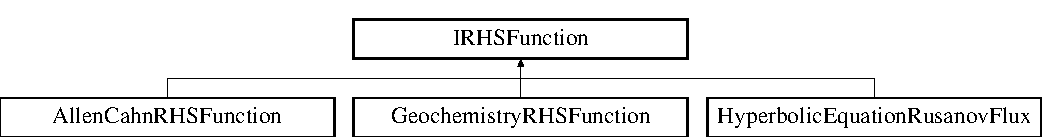
\includegraphics[height=1.83908cm]{classIRHSFunction}
\end{center}
\end{figure}
\subsection*{Public Member Functions}
\begin{DoxyCompactItemize}
\item 
\hypertarget{classIRHSFunction_a0ba33a3b44f77c7f51c3ce085ecbd003}{
virtual RealVector {\bfseries evalF} (Real time, RealVector \&y)=0}
\label{classIRHSFunction_a0ba33a3b44f77c7f51c3ce085ecbd003}

\item 
\hypertarget{classIRHSFunction_a5f28c5fe8ffde86f839e859cd2fb6424}{
virtual RealVector {\bfseries evalF} (Real time, RealVector \&y, IntegerVector \&ref)=0}
\label{classIRHSFunction_a5f28c5fe8ffde86f839e859cd2fb6424}

\item 
\hypertarget{classIRHSFunction_af82bf63b0230781d0936825c97ac15cc}{
virtual RealMatrixSparse {\bfseries evaldFdY} (Real time, RealVector \&y)=0}
\label{classIRHSFunction_af82bf63b0230781d0936825c97ac15cc}

\item 
\hypertarget{classIRHSFunction_a4e4676728e8141f7dc956e061e6468c4}{
virtual RealMatrixSparse {\bfseries evaldFdY} (Real time, RealVector \&y, IntegerVector \&ref)=0}
\label{classIRHSFunction_a4e4676728e8141f7dc956e061e6468c4}

\end{DoxyCompactItemize}


The documentation for this class was generated from the following file:\begin{DoxyCompactItemize}
\item 
IRHSFunction.h\end{DoxyCompactItemize}

\hypertarget{classISolverData}{
\section{ISolverData Class Reference}
\label{classISolverData}\index{ISolverData@{ISolverData}}
}
Inheritance diagram for ISolverData::\begin{figure}[H]
\begin{center}
\leavevmode
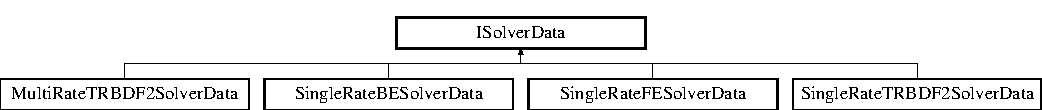
\includegraphics[height=1.47368cm]{classISolverData}
\end{center}
\end{figure}
\subsection*{Public Member Functions}
\begin{DoxyCompactItemize}
\item 
\hypertarget{classISolverData_ac9bd0d0902bf6c7a47d1b82097e734b9}{
virtual const RealVector \& {\bfseries getError} () const =0}
\label{classISolverData_ac9bd0d0902bf6c7a47d1b82097e734b9}

\item 
\hypertarget{classISolverData_adf0c47be80ef98e377e2bcc99ce1ecae}{
virtual void {\bfseries setError} (const RealVector \&error)=0}
\label{classISolverData_adf0c47be80ef98e377e2bcc99ce1ecae}

\item 
\hypertarget{classISolverData_addcac56958d8b75157a19cf3046ddbed}{
virtual Real {\bfseries getH} () const =0}
\label{classISolverData_addcac56958d8b75157a19cf3046ddbed}

\item 
\hypertarget{classISolverData_acdfe4a78fbb4919abc4151afe355d786}{
virtual void {\bfseries setH} (Real h)=0}
\label{classISolverData_acdfe4a78fbb4919abc4151afe355d786}

\item 
\hypertarget{classISolverData_ae4f2dee77edb21d09aa139538499f6f9}{
virtual Bool {\bfseries isHasSucceded} () const =0}
\label{classISolverData_ae4f2dee77edb21d09aa139538499f6f9}

\item 
\hypertarget{classISolverData_ac3e1f3066da46cf8f1835bc7f472cb8e}{
virtual void {\bfseries setHasSucceded} (Bool hasSucceded)=0}
\label{classISolverData_ac3e1f3066da46cf8f1835bc7f472cb8e}

\item 
\hypertarget{classISolverData_ae828c5447215a66209c5aac4a4f41cb1}{
virtual Real {\bfseries getTime} () const =0}
\label{classISolverData_ae828c5447215a66209c5aac4a4f41cb1}

\item 
\hypertarget{classISolverData_a447682e1f88025ed4f9ecd0a51b3e268}{
virtual void {\bfseries setTime} (Real time)=0}
\label{classISolverData_a447682e1f88025ed4f9ecd0a51b3e268}

\item 
\hypertarget{classISolverData_ade791cc49459d83f06c2af28444355b3}{
virtual const RealVector \& {\bfseries getY} () const =0}
\label{classISolverData_ade791cc49459d83f06c2af28444355b3}

\item 
\hypertarget{classISolverData_a502bbea5e7ee8a30e931225e2b688d53}{
virtual void {\bfseries setY} (const RealVector \&y)=0}
\label{classISolverData_a502bbea5e7ee8a30e931225e2b688d53}

\item 
\hypertarget{classISolverData_ad70dc78009a260f66ec6f1f70595b6e2}{
virtual const IntegerVector \& {\bfseries getMesh} () const =0}
\label{classISolverData_ad70dc78009a260f66ec6f1f70595b6e2}

\item 
\hypertarget{classISolverData_a92ab1d515b4821bef0baa4c9aa1329b2}{
virtual void {\bfseries setMesh} (const IntegerVector \&mesh)=0}
\label{classISolverData_a92ab1d515b4821bef0baa4c9aa1329b2}

\item 
\hypertarget{classISolverData_a13a702e8d1bbabe4fcdd1fefceac540b}{
virtual Bool {\bfseries isRefining} () const =0}
\label{classISolverData_a13a702e8d1bbabe4fcdd1fefceac540b}

\item 
\hypertarget{classISolverData_a00920a57269b67f4b381e98fe98bd77b}{
virtual void {\bfseries setRefining} (Bool refining)=0}
\label{classISolverData_a00920a57269b67f4b381e98fe98bd77b}

\item 
\hypertarget{classISolverData_a9b5aafd177911c1b61d5ae880c4cef3b}{
virtual const IntegerVector \& {\bfseries getNumbComponentsSolve} () const =0}
\label{classISolverData_a9b5aafd177911c1b61d5ae880c4cef3b}

\item 
\hypertarget{classISolverData_a1bc63351b238535b4e73649ef237a53c}{
virtual void {\bfseries setNumbComponentsSolve} (const IntegerVector \&numbComponentsSolve)=0}
\label{classISolverData_a1bc63351b238535b4e73649ef237a53c}

\end{DoxyCompactItemize}


The documentation for this class was generated from the following file:\begin{DoxyCompactItemize}
\item 
ISolverData.h\end{DoxyCompactItemize}

\hypertarget{classLinearFluxFunction}{
\section{LinearFluxFunction Class Reference}
\label{classLinearFluxFunction}\index{LinearFluxFunction@{LinearFluxFunction}}
}


Linear flux for the Hyperbolic PDE.  


{\ttfamily \#include $<$LinearFluxFunction.h$>$}Inheritance diagram for LinearFluxFunction::\begin{figure}[H]
\begin{center}
\leavevmode
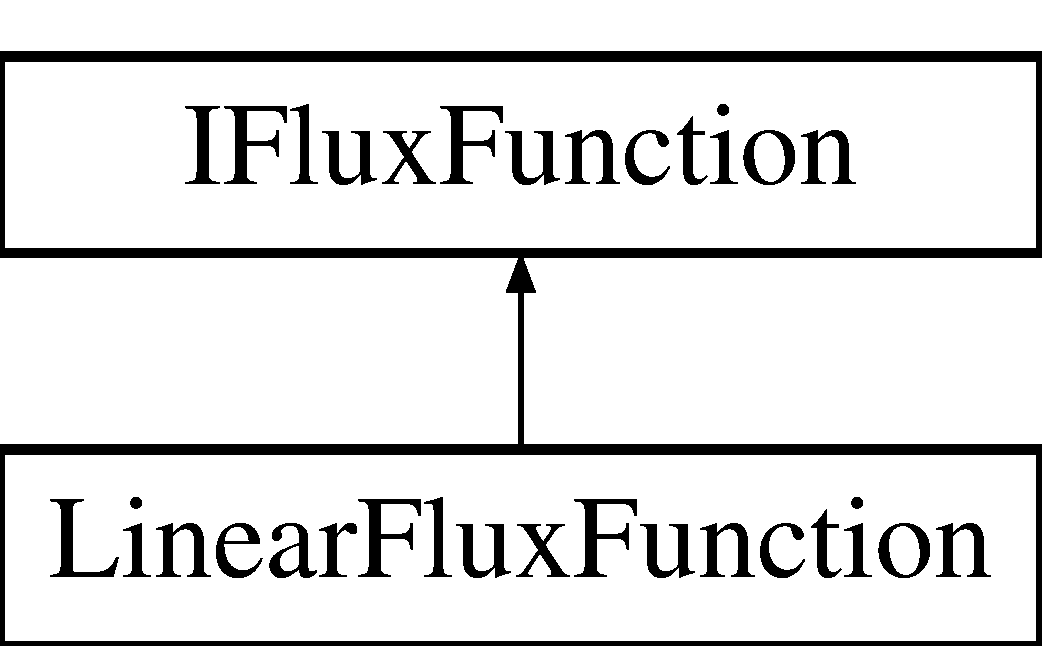
\includegraphics[height=2cm]{classLinearFluxFunction}
\end{center}
\end{figure}
\subsection*{Public Member Functions}
\begin{DoxyCompactItemize}
\item 
\hypertarget{classLinearFluxFunction_a7ed546c493111d905b74f21525dba6aa}{
Real {\bfseries getA} () const }
\label{classLinearFluxFunction_a7ed546c493111d905b74f21525dba6aa}

\item 
\hypertarget{classLinearFluxFunction_a56fac54d5cff803b220ce6e07e90d8ef}{
void {\bfseries setA} (Real a)}
\label{classLinearFluxFunction_a56fac54d5cff803b220ce6e07e90d8ef}

\item 
\hypertarget{classLinearFluxFunction_a31a0643b300312e983e81cba2369ddc0}{
Real \hyperlink{classLinearFluxFunction_a31a0643b300312e983e81cba2369ddc0}{evalF} (Real time, Real y\_\-sol)}
\label{classLinearFluxFunction_a31a0643b300312e983e81cba2369ddc0}

\begin{DoxyCompactList}\small\item\em Evaluates the flux function component by component, we can't put as input a vector. \item\end{DoxyCompactList}\item 
\hypertarget{classLinearFluxFunction_a0091e8fac858703d344ca66d108f1b39}{
Real {\bfseries evalFderivative} (Real time, Real y\_\-sol)}
\label{classLinearFluxFunction_a0091e8fac858703d344ca66d108f1b39}

\end{DoxyCompactItemize}


\subsection{Detailed Description}
Linear flux for the Hyperbolic PDE. $ f(u) = au(x,t) $ 

The documentation for this class was generated from the following files:\begin{DoxyCompactItemize}
\item 
HyperbolicEquationUpwindRHSFunction/LinearFluxFunction.h\item 
HyperbolicEquationUpwindRHSFunction/LinearFluxFunction.cpp\end{DoxyCompactItemize}

\hypertarget{classMasterSolution}{
\section{MasterSolution Class Reference}
\label{classMasterSolution}\index{MasterSolution@{MasterSolution}}
}


Class useful to store only some information from the SolverData class.  


{\ttfamily \#include $<$MasterSolution.h$>$}\subsection*{Public Member Functions}
\begin{DoxyCompactItemize}
\item 
\hypertarget{classMasterSolution_a5636ad5be535ed1d73f23862b70bf0f8}{
Real {\bfseries getT} () const }
\label{classMasterSolution_a5636ad5be535ed1d73f23862b70bf0f8}

\item 
\hypertarget{classMasterSolution_aab93fbe3e24d67549d22ff7cdf879b84}{
void {\bfseries setT} (Real t)}
\label{classMasterSolution_aab93fbe3e24d67549d22ff7cdf879b84}

\item 
\hypertarget{classMasterSolution_a3c51bf00996eb64b35722b329d86768a}{
const RealVector \& {\bfseries getY} () const }
\label{classMasterSolution_a3c51bf00996eb64b35722b329d86768a}

\item 
\hypertarget{classMasterSolution_a16075bff7c2b04a0f5638ee6c491eb62}{
void {\bfseries setY} (const RealVector \&y)}
\label{classMasterSolution_a16075bff7c2b04a0f5638ee6c491eb62}

\end{DoxyCompactItemize}


\subsection{Detailed Description}
Class useful to store only some information from the SolverData class. 

The documentation for this class was generated from the following files:\begin{DoxyCompactItemize}
\item 
MasterSolverOutputManipulator/MasterSolution.h\item 
MasterSolverOutputManipulator/MasterSolution.cpp\end{DoxyCompactItemize}

\hypertarget{classMultiRateTRBDF2Solver}{
\section{MultiRateTRBDF2Solver Class Reference}
\label{classMultiRateTRBDF2Solver}\index{MultiRateTRBDF2Solver@{MultiRateTRBDF2Solver}}
}
Inheritance diagram for MultiRateTRBDF2Solver::\begin{figure}[H]
\begin{center}
\leavevmode
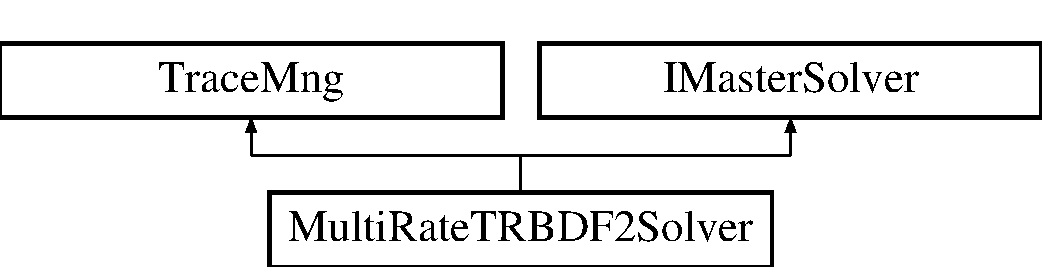
\includegraphics[height=2cm]{classMultiRateTRBDF2Solver}
\end{center}
\end{figure}
\subsection*{Public Member Functions}
\begin{DoxyCompactItemize}
\item 
\hypertarget{classMultiRateTRBDF2Solver_abba38b276958ca27b4da6dc05810198e}{
void \hyperlink{classMultiRateTRBDF2Solver_abba38b276958ca27b4da6dc05810198e}{setFun} (\hyperlink{classIRHSFunction}{IRHSFunction} $\ast$fun)}
\label{classMultiRateTRBDF2Solver_abba38b276958ca27b4da6dc05810198e}

\begin{DoxyCompactList}\small\item\em Sets the RHS Function. \item\end{DoxyCompactList}\item 
\hypertarget{classMultiRateTRBDF2Solver_a2975901caa9b3e8307876e420d11051a}{
void \hyperlink{classMultiRateTRBDF2Solver_a2975901caa9b3e8307876e420d11051a}{setNewtSolv} (std::unique\_\-ptr$<$ \hyperlink{classINewtonSolver}{INewtonSolver} $>$ newtSolv)}
\label{classMultiRateTRBDF2Solver_a2975901caa9b3e8307876e420d11051a}

\begin{DoxyCompactList}\small\item\em Sets the Newton SOlver. \item\end{DoxyCompactList}\item 
\hypertarget{classMultiRateTRBDF2Solver_a108e0f1d57fa5fcf7c0a256b73de9b46}{
void \hyperlink{classMultiRateTRBDF2Solver_a108e0f1d57fa5fcf7c0a256b73de9b46}{setHinitial} (Real hinitial)}
\label{classMultiRateTRBDF2Solver_a108e0f1d57fa5fcf7c0a256b73de9b46}

\begin{DoxyCompactList}\small\item\em Sets the time step for the first time slab. \item\end{DoxyCompactList}\item 
\hypertarget{classMultiRateTRBDF2Solver_a6849c58254a896d35a473e180bce8ca7}{
void \hyperlink{classMultiRateTRBDF2Solver_a6849c58254a896d35a473e180bce8ca7}{setHz1initial} (const RealVector \&hz1initial)}
\label{classMultiRateTRBDF2Solver_a6849c58254a896d35a473e180bce8ca7}

\begin{DoxyCompactList}\small\item\em Sets the initial guess for the variable z. \item\end{DoxyCompactList}\item 
\hypertarget{classMultiRateTRBDF2Solver_a4cbd43086b77c41081b94316b6c0c0fa}{
void \hyperlink{classMultiRateTRBDF2Solver_a4cbd43086b77c41081b94316b6c0c0fa}{setTfinal} (Real tfinal)}
\label{classMultiRateTRBDF2Solver_a4cbd43086b77c41081b94316b6c0c0fa}

\begin{DoxyCompactList}\small\item\em Sets the final time. \item\end{DoxyCompactList}\item 
\hypertarget{classMultiRateTRBDF2Solver_a2414fae818f613f1d22c2cbc9d3874a2}{
void \hyperlink{classMultiRateTRBDF2Solver_a2414fae818f613f1d22c2cbc9d3874a2}{setTinitial} (Real tinitial)}
\label{classMultiRateTRBDF2Solver_a2414fae818f613f1d22c2cbc9d3874a2}

\begin{DoxyCompactList}\small\item\em Sets the initial time. \item\end{DoxyCompactList}\item 
\hypertarget{classMultiRateTRBDF2Solver_a80c6f99043ef743e40ce3281a6e5f078}{
void \hyperlink{classMultiRateTRBDF2Solver_a80c6f99043ef743e40ce3281a6e5f078}{setYinitial} (const RealVector \&yinitial)}
\label{classMultiRateTRBDF2Solver_a80c6f99043ef743e40ce3281a6e5f078}

\begin{DoxyCompactList}\small\item\em Sets the initial condition. \item\end{DoxyCompactList}\item 
\hypertarget{classMultiRateTRBDF2Solver_a5f31da03700507626779ef83441b8108}{
std::vector$<$ std::unique\_\-ptr$<$ \hyperlink{classISolverData}{ISolverData} $>$ $>$ \&\& \hyperlink{classMultiRateTRBDF2Solver_a5f31da03700507626779ef83441b8108}{getSolution} ()}
\label{classMultiRateTRBDF2Solver_a5f31da03700507626779ef83441b8108}

\begin{DoxyCompactList}\small\item\em Gets the solution vector. \item\end{DoxyCompactList}\item 
\hypertarget{classMultiRateTRBDF2Solver_aa7a96662dd73f626b2c33f6f16f7e531}{
void \hyperlink{classMultiRateTRBDF2Solver_aa7a96662dd73f626b2c33f6f16f7e531}{setNewtonTolAbs} (Real newtonTolAbs)}
\label{classMultiRateTRBDF2Solver_aa7a96662dd73f626b2c33f6f16f7e531}

\begin{DoxyCompactList}\small\item\em Sets the absolute Newton tolerance. \item\end{DoxyCompactList}\item 
\hypertarget{classMultiRateTRBDF2Solver_a6c5ba21c5ede4e7915898c1ef705b422}{
void \hyperlink{classMultiRateTRBDF2Solver_a6c5ba21c5ede4e7915898c1ef705b422}{setNewtonTolRel} (Real newtonTolRel)}
\label{classMultiRateTRBDF2Solver_a6c5ba21c5ede4e7915898c1ef705b422}

\begin{DoxyCompactList}\small\item\em Sets the relative Newton tolerance. \item\end{DoxyCompactList}\item 
\hypertarget{classMultiRateTRBDF2Solver_a43c3ea4cdada6de697ab40d85c1ad98b}{
void \hyperlink{classMultiRateTRBDF2Solver_a43c3ea4cdada6de697ab40d85c1ad98b}{setErrorTolAbs} (Real errorTolAbs)}
\label{classMultiRateTRBDF2Solver_a43c3ea4cdada6de697ab40d85c1ad98b}

\begin{DoxyCompactList}\small\item\em Sets the absolute Error tolerance. \item\end{DoxyCompactList}\item 
\hypertarget{classMultiRateTRBDF2Solver_aeb42ae9c8fd687d080987d2b19b28c4a}{
void \hyperlink{classMultiRateTRBDF2Solver_aeb42ae9c8fd687d080987d2b19b28c4a}{setErrorTolRel} (Real errorTolRel)}
\label{classMultiRateTRBDF2Solver_aeb42ae9c8fd687d080987d2b19b28c4a}

\begin{DoxyCompactList}\small\item\em Sets the relative Error tolerance. \item\end{DoxyCompactList}\item 
void \hyperlink{classMultiRateTRBDF2Solver_af938aabdcfc8c26f802fa648812e83cc}{compute} ()
\end{DoxyCompactItemize}


\subsection{Member Function Documentation}
\hypertarget{classMultiRateTRBDF2Solver_af938aabdcfc8c26f802fa648812e83cc}{
\index{MultiRateTRBDF2Solver@{MultiRateTRBDF2Solver}!compute@{compute}}
\index{compute@{compute}!MultiRateTRBDF2Solver@{MultiRateTRBDF2Solver}}
\subsubsection[{compute}]{\setlength{\rightskip}{0pt plus 5cm}void MultiRateTRBDF2Solver::compute ()\hspace{0.3cm}{\ttfamily  \mbox{[}virtual\mbox{]}}}}
\label{classMultiRateTRBDF2Solver_af938aabdcfc8c26f802fa648812e83cc}


Calculate the solution with TRBDF2 Method

we are in a sub-\/level we have to do the interpolation

Compute Standard Stiff Problem Estimator

Calculate if the time step has succeded and if we have some components that should be refine

Store the numerical Solution and update values

store the values that we need for the interpolation

update the values that we need for the interpolation

Propose next time step

if we don't accept the time step we calculate a small one

we accept the time step and it is not necessary to refine

Propose next time step

Special case: we exit from a sub-\/level that has the same t-\/final of the previous one or more than one. we have to update the initial condition (hz) and we have to eliminate the variables of the forward sub-\/levels.

Propose next time step 

Implements \hyperlink{classIMasterSolver}{IMasterSolver}.

The documentation for this class was generated from the following files:\begin{DoxyCompactItemize}
\item 
MultiRateTRBDF2Solver/MultiRateTRBDF2Solver.h\item 
MultiRateTRBDF2Solver/MultiRateTRBDF2Solver.cpp\end{DoxyCompactItemize}

\hypertarget{classMultiRateTRBDF2SolverData}{
\section{MultiRateTRBDF2SolverData Class Reference}
\label{classMultiRateTRBDF2SolverData}\index{MultiRateTRBDF2SolverData@{MultiRateTRBDF2SolverData}}
}
Inheritance diagram for MultiRateTRBDF2SolverData::\begin{figure}[H]
\begin{center}
\leavevmode
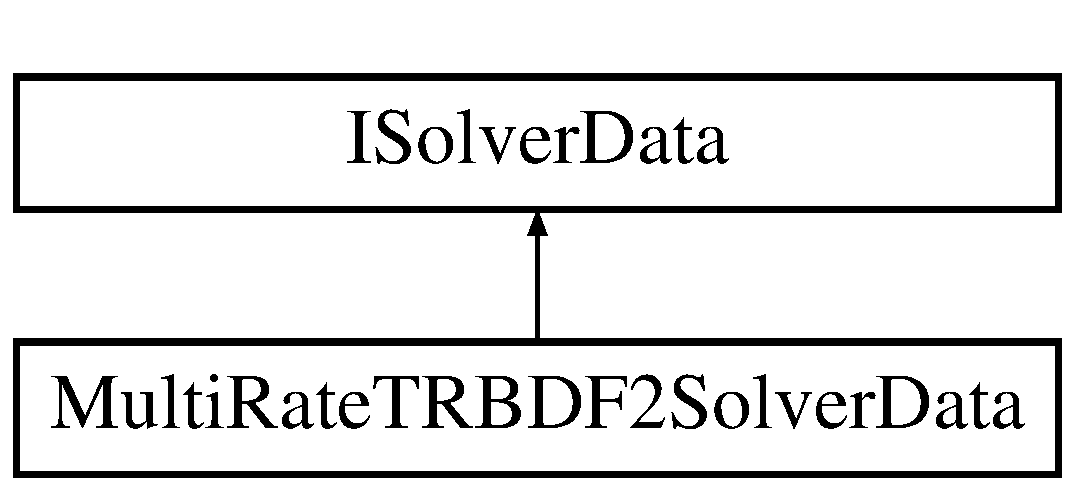
\includegraphics[height=2cm]{classMultiRateTRBDF2SolverData}
\end{center}
\end{figure}
\subsection*{Public Member Functions}
\begin{DoxyCompactItemize}
\item 
\hypertarget{classMultiRateTRBDF2SolverData_a310271deced3d51c8142442f154f38fd}{
const RealVector \& \hyperlink{classMultiRateTRBDF2SolverData_a310271deced3d51c8142442f154f38fd}{getError} () const }
\label{classMultiRateTRBDF2SolverData_a310271deced3d51c8142442f154f38fd}

\begin{DoxyCompactList}\small\item\em Gets the error estimation. \item\end{DoxyCompactList}\item 
\hypertarget{classMultiRateTRBDF2SolverData_a9086199e30afc0863574c87867f56c1f}{
void \hyperlink{classMultiRateTRBDF2SolverData_a9086199e30afc0863574c87867f56c1f}{setError} (const RealVector \&error)}
\label{classMultiRateTRBDF2SolverData_a9086199e30afc0863574c87867f56c1f}

\begin{DoxyCompactList}\small\item\em Sets the error estimation. \item\end{DoxyCompactList}\item 
\hypertarget{classMultiRateTRBDF2SolverData_a088daa942d6ec822d5799e7d67381b39}{
Real \hyperlink{classMultiRateTRBDF2SolverData_a088daa942d6ec822d5799e7d67381b39}{getH} () const }
\label{classMultiRateTRBDF2SolverData_a088daa942d6ec822d5799e7d67381b39}

\begin{DoxyCompactList}\small\item\em Gets the size of the time step. \item\end{DoxyCompactList}\item 
\hypertarget{classMultiRateTRBDF2SolverData_a8e01b1c6a54135cb30b16ec35750750a}{
void \hyperlink{classMultiRateTRBDF2SolverData_a8e01b1c6a54135cb30b16ec35750750a}{setH} (Real h)}
\label{classMultiRateTRBDF2SolverData_a8e01b1c6a54135cb30b16ec35750750a}

\begin{DoxyCompactList}\small\item\em Sets the size of the time step. \item\end{DoxyCompactList}\item 
\hypertarget{classMultiRateTRBDF2SolverData_a3e9cc3df9e7344c6b4161c6e5dd492c3}{
Bool \hyperlink{classMultiRateTRBDF2SolverData_a3e9cc3df9e7344c6b4161c6e5dd492c3}{isHasSucceded} () const }
\label{classMultiRateTRBDF2SolverData_a3e9cc3df9e7344c6b4161c6e5dd492c3}

\begin{DoxyCompactList}\small\item\em Gets the boolean variable that says if the time step is accepted. \item\end{DoxyCompactList}\item 
\hypertarget{classMultiRateTRBDF2SolverData_aea944caae448918e895d7a70e45654d0}{
void \hyperlink{classMultiRateTRBDF2SolverData_aea944caae448918e895d7a70e45654d0}{setHasSucceded} (Bool hasSucceded)}
\label{classMultiRateTRBDF2SolverData_aea944caae448918e895d7a70e45654d0}

\begin{DoxyCompactList}\small\item\em Sets the boolean variable that says if the time step is accepted. \item\end{DoxyCompactList}\item 
\hypertarget{classMultiRateTRBDF2SolverData_aa6a3f6cd8e12b7ab453c9a799895c21f}{
Real \hyperlink{classMultiRateTRBDF2SolverData_aa6a3f6cd8e12b7ab453c9a799895c21f}{getTime} () const }
\label{classMultiRateTRBDF2SolverData_aa6a3f6cd8e12b7ab453c9a799895c21f}

\begin{DoxyCompactList}\small\item\em Gets the time where is computed the solution. \item\end{DoxyCompactList}\item 
\hypertarget{classMultiRateTRBDF2SolverData_a17fe220be0669beab144a72122518147}{
void \hyperlink{classMultiRateTRBDF2SolverData_a17fe220be0669beab144a72122518147}{setTime} (Real time)}
\label{classMultiRateTRBDF2SolverData_a17fe220be0669beab144a72122518147}

\begin{DoxyCompactList}\small\item\em Sets the time where is computed the solution. \item\end{DoxyCompactList}\item 
\hypertarget{classMultiRateTRBDF2SolverData_aa3c3459d54c5f0e2c1236062ec0d422a}{
const RealVector \& \hyperlink{classMultiRateTRBDF2SolverData_aa3c3459d54c5f0e2c1236062ec0d422a}{getY} () const }
\label{classMultiRateTRBDF2SolverData_aa3c3459d54c5f0e2c1236062ec0d422a}

\begin{DoxyCompactList}\small\item\em Gets the solution. \item\end{DoxyCompactList}\item 
\hypertarget{classMultiRateTRBDF2SolverData_af1233e2d355383e2ccf14341a6c690d7}{
void \hyperlink{classMultiRateTRBDF2SolverData_af1233e2d355383e2ccf14341a6c690d7}{setY} (const RealVector \&y)}
\label{classMultiRateTRBDF2SolverData_af1233e2d355383e2ccf14341a6c690d7}

\begin{DoxyCompactList}\small\item\em Sets the solution. \item\end{DoxyCompactList}\item 
\hypertarget{classMultiRateTRBDF2SolverData_ab3a002810c0bdf01fe2daebe7f309d58}{
const IntegerVector \& \hyperlink{classMultiRateTRBDF2SolverData_ab3a002810c0bdf01fe2daebe7f309d58}{getMesh} () const }
\label{classMultiRateTRBDF2SolverData_ab3a002810c0bdf01fe2daebe7f309d58}

\begin{DoxyCompactList}\small\item\em Gets the mesh vector, useful to see the active and latent components. \item\end{DoxyCompactList}\item 
\hypertarget{classMultiRateTRBDF2SolverData_a08dd24d9391710fa80d3f2d00f157dfe}{
void \hyperlink{classMultiRateTRBDF2SolverData_a08dd24d9391710fa80d3f2d00f157dfe}{setMesh} (const IntegerVector \&mesh)}
\label{classMultiRateTRBDF2SolverData_a08dd24d9391710fa80d3f2d00f157dfe}

\begin{DoxyCompactList}\small\item\em Sets the mesh vector, useful to see the active and latent components. \item\end{DoxyCompactList}\item 
\hypertarget{classMultiRateTRBDF2SolverData_a57d58fc11fd5421bb40446db15fba4e3}{
Bool \hyperlink{classMultiRateTRBDF2SolverData_a57d58fc11fd5421bb40446db15fba4e3}{isRefining} () const }
\label{classMultiRateTRBDF2SolverData_a57d58fc11fd5421bb40446db15fba4e3}

\begin{DoxyCompactList}\small\item\em Gets the boolean value refining, it is true if we have to refine the time step. \item\end{DoxyCompactList}\item 
\hypertarget{classMultiRateTRBDF2SolverData_ac8152b7b7603e631afbd58b689615eaa}{
void \hyperlink{classMultiRateTRBDF2SolverData_ac8152b7b7603e631afbd58b689615eaa}{setRefining} (Bool refining)}
\label{classMultiRateTRBDF2SolverData_ac8152b7b7603e631afbd58b689615eaa}

\begin{DoxyCompactList}\small\item\em Sets the boolean value refining, it is true if we have to refine the time step. \item\end{DoxyCompactList}\item 
const IntegerVector \& \hyperlink{classMultiRateTRBDF2SolverData_ad8c376746e1daddc1f3ecc6986206c79}{getNumbComponentsSolve} () const 
\item 
\hypertarget{classMultiRateTRBDF2SolverData_a756db2ce93a3dfd2d24f0eb524d7e87b}{
void \hyperlink{classMultiRateTRBDF2SolverData_a756db2ce93a3dfd2d24f0eb524d7e87b}{setNumbComponentsSolve} (const IntegerVector \&numbComponentsSolve)}
\label{classMultiRateTRBDF2SolverData_a756db2ce93a3dfd2d24f0eb524d7e87b}

\begin{DoxyCompactList}\small\item\em Sets the vector NumbComponentsSolve. \item\end{DoxyCompactList}\end{DoxyCompactItemize}


\subsection{Member Function Documentation}
\hypertarget{classMultiRateTRBDF2SolverData_ad8c376746e1daddc1f3ecc6986206c79}{
\index{MultiRateTRBDF2SolverData@{MultiRateTRBDF2SolverData}!getNumbComponentsSolve@{getNumbComponentsSolve}}
\index{getNumbComponentsSolve@{getNumbComponentsSolve}!MultiRateTRBDF2SolverData@{MultiRateTRBDF2SolverData}}
\subsubsection[{getNumbComponentsSolve}]{\setlength{\rightskip}{0pt plus 5cm}const IntegerVector \& MultiRateTRBDF2SolverData::getNumbComponentsSolve () const\hspace{0.3cm}{\ttfamily  \mbox{[}virtual\mbox{]}}}}
\label{classMultiRateTRBDF2SolverData_ad8c376746e1daddc1f3ecc6986206c79}
Gets a vector of 0 and 1(if for the i-\/th component it is equal to 1 means that we are computed the solution with the TRBDF2 method, if it is equal to 0 it means that we are interpolating that component's solution) 

Implements \hyperlink{classISolverData}{ISolverData}.

The documentation for this class was generated from the following files:\begin{DoxyCompactItemize}
\item 
MultiRateTRBDF2Solver/MultiRateTRBDF2SolverData.h\item 
MultiRateTRBDF2Solver/MultiRateTRBDF2SolverData.cpp\end{DoxyCompactItemize}

\hypertarget{classNulOStream}{
\section{NulOStream Class Reference}
\label{classNulOStream}\index{NulOStream@{NulOStream}}
}
Inheritance diagram for NulOStream::\begin{figure}[H]
\begin{center}
\leavevmode
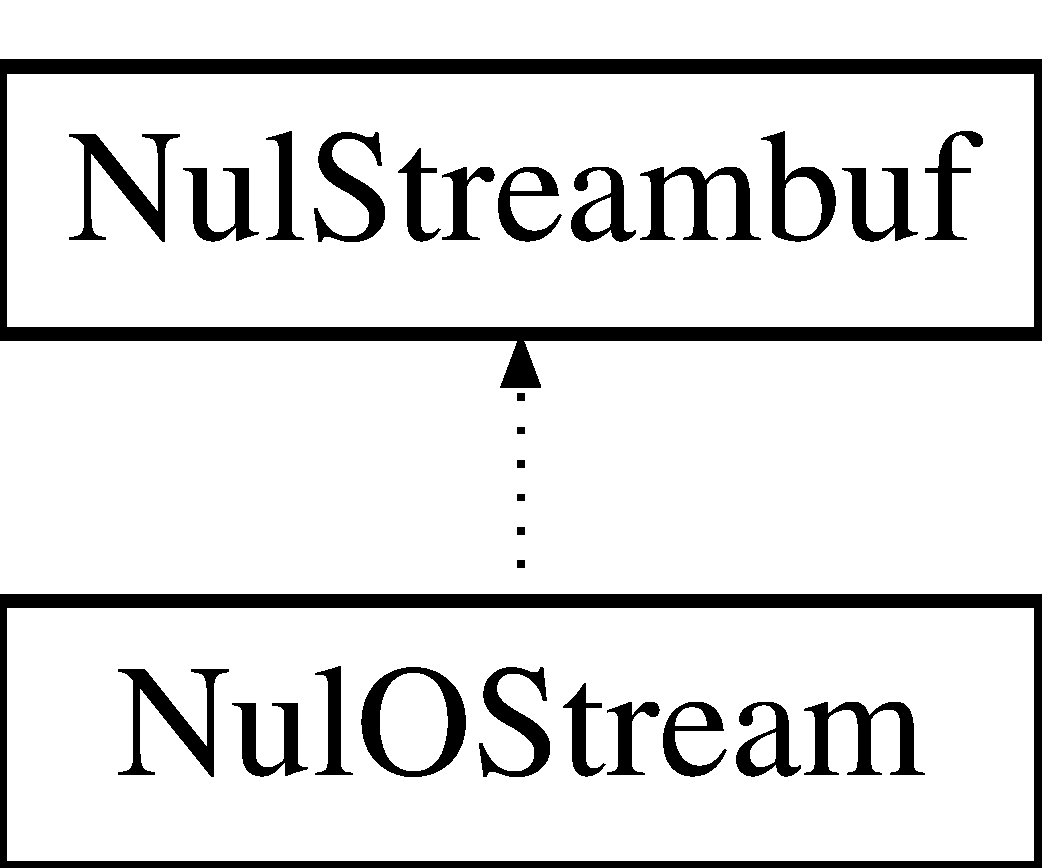
\includegraphics[height=2cm]{classNulOStream}
\end{center}
\end{figure}
\subsection*{Public Member Functions}
\begin{DoxyCompactItemize}
\item 
\hypertarget{classNulOStream_adf32a85d4d53e7dfcb0e5d8ee259513b}{
\hyperlink{classNulStreambuf}{NulStreambuf} $\ast$ {\bfseries rdbuf} ()}
\label{classNulOStream_adf32a85d4d53e7dfcb0e5d8ee259513b}

\end{DoxyCompactItemize}


The documentation for this class was generated from the following file:\begin{DoxyCompactItemize}
\item 
TraceMng.h\end{DoxyCompactItemize}

\hypertarget{classNulStreambuf}{
\section{NulStreambuf Class Reference}
\label{classNulStreambuf}\index{NulStreambuf@{NulStreambuf}}
}
Inheritance diagram for NulStreambuf::\begin{figure}[H]
\begin{center}
\leavevmode
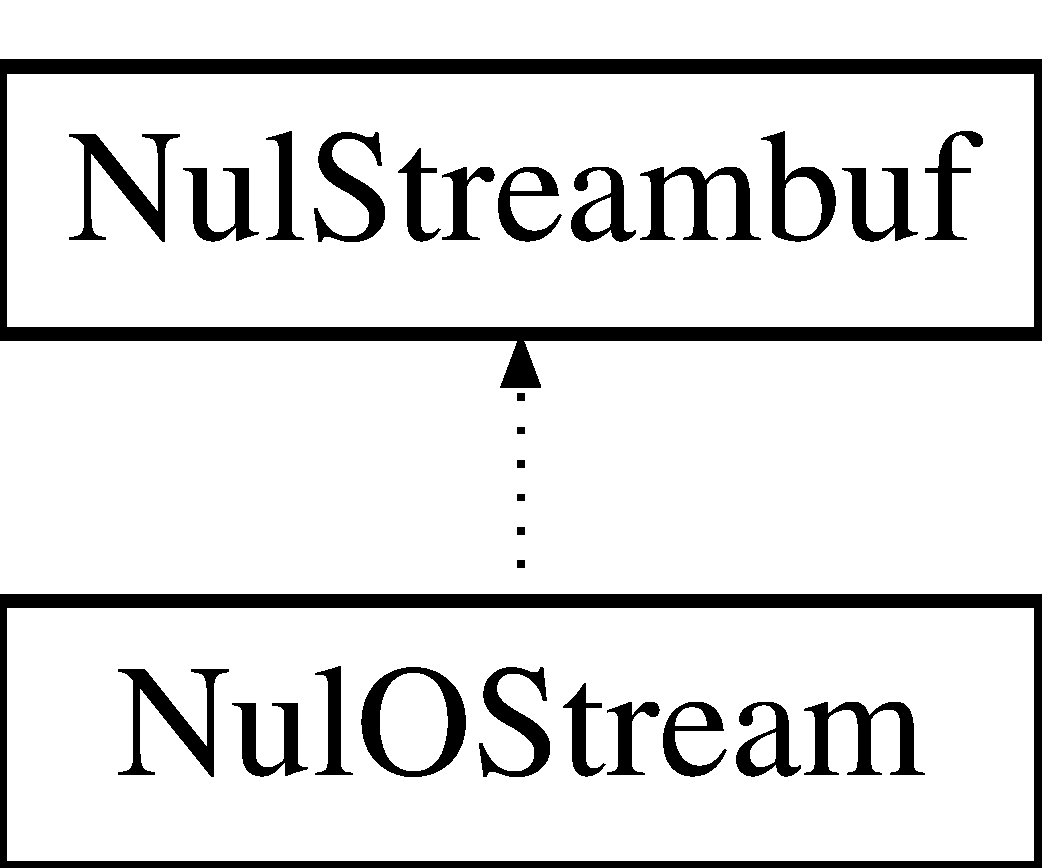
\includegraphics[height=2cm]{classNulStreambuf}
\end{center}
\end{figure}
\subsection*{Protected Member Functions}
\begin{DoxyCompactItemize}
\item 
\hypertarget{classNulStreambuf_aeaba3d336743d4c7bd8a2ca254dfcac4}{
virtual int {\bfseries overflow} (int c)}
\label{classNulStreambuf_aeaba3d336743d4c7bd8a2ca254dfcac4}

\end{DoxyCompactItemize}


The documentation for this class was generated from the following file:\begin{DoxyCompactItemize}
\item 
TraceMng.h\end{DoxyCompactItemize}

\hypertarget{classSingleRateBESolver}{
\section{SingleRateBESolver Class Reference}
\label{classSingleRateBESolver}\index{SingleRateBESolver@{SingleRateBESolver}}
}


Class to define the Singlerate Backward Euler Solver with a fixed time step.  


{\ttfamily \#include $<$SingleRateBESolver.h$>$}Inheritance diagram for SingleRateBESolver::\begin{figure}[H]
\begin{center}
\leavevmode
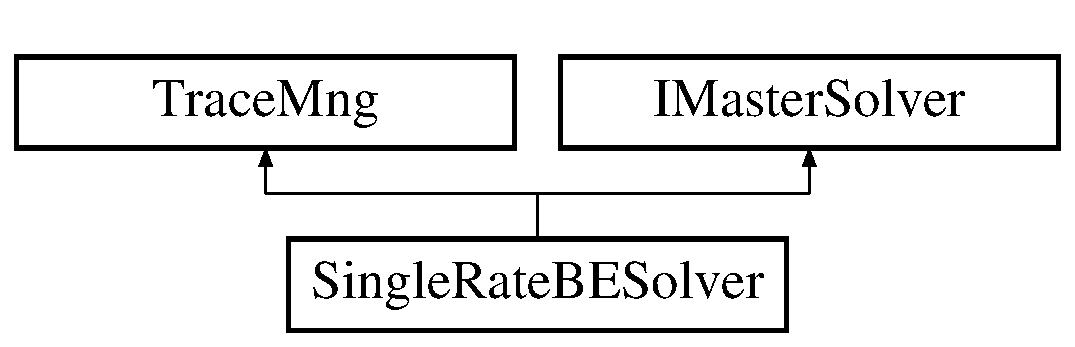
\includegraphics[height=2cm]{classSingleRateBESolver}
\end{center}
\end{figure}
\subsection*{Public Member Functions}
\begin{DoxyCompactItemize}
\item 
\hypertarget{classSingleRateBESolver_ab62ae4e0720cd64397b9a3b2795f295b}{
void \hyperlink{classSingleRateBESolver_ab62ae4e0720cd64397b9a3b2795f295b}{setFun} (\hyperlink{classIRHSFunction}{IRHSFunction} $\ast$fun)}
\label{classSingleRateBESolver_ab62ae4e0720cd64397b9a3b2795f295b}

\begin{DoxyCompactList}\small\item\em Sets the RHS Function. \item\end{DoxyCompactList}\item 
\hypertarget{classSingleRateBESolver_aa870a6088429e48ea68e82e57aed170f}{
void \hyperlink{classSingleRateBESolver_aa870a6088429e48ea68e82e57aed170f}{setNewtSolv} (std::unique\_\-ptr$<$ \hyperlink{classINewtonSolver}{INewtonSolver} $>$ newtSolv)}
\label{classSingleRateBESolver_aa870a6088429e48ea68e82e57aed170f}

\begin{DoxyCompactList}\small\item\em Sets the Newton SOlver. \item\end{DoxyCompactList}\item 
\hypertarget{classSingleRateBESolver_a8e5175349db542325d3018425b697a57}{
void \hyperlink{classSingleRateBESolver_a8e5175349db542325d3018425b697a57}{setHinitial} (Real hinitial)}
\label{classSingleRateBESolver_a8e5175349db542325d3018425b697a57}

\begin{DoxyCompactList}\small\item\em Sets the time step for the first time slab. \item\end{DoxyCompactList}\item 
\hypertarget{classSingleRateBESolver_ad4f25d37e24a0ffca299be5b883bda7f}{
void \hyperlink{classSingleRateBESolver_ad4f25d37e24a0ffca299be5b883bda7f}{setHz1initial} (const RealVector \&hz1initial)}
\label{classSingleRateBESolver_ad4f25d37e24a0ffca299be5b883bda7f}

\begin{DoxyCompactList}\small\item\em Sets the initial guess for the variable z. \item\end{DoxyCompactList}\item 
\hypertarget{classSingleRateBESolver_ab0f8f8e6acf3caf0fc71c96f6453f645}{
void \hyperlink{classSingleRateBESolver_ab0f8f8e6acf3caf0fc71c96f6453f645}{setTfinal} (Real tfinal)}
\label{classSingleRateBESolver_ab0f8f8e6acf3caf0fc71c96f6453f645}

\begin{DoxyCompactList}\small\item\em Sets the final time. \item\end{DoxyCompactList}\item 
\hypertarget{classSingleRateBESolver_a980cdd2a991061325ea33d1107625894}{
void \hyperlink{classSingleRateBESolver_a980cdd2a991061325ea33d1107625894}{setTinitial} (Real tinitial)}
\label{classSingleRateBESolver_a980cdd2a991061325ea33d1107625894}

\begin{DoxyCompactList}\small\item\em Sets the initial time. \item\end{DoxyCompactList}\item 
\hypertarget{classSingleRateBESolver_a17249255931cafae0630af063b79a31b}{
void \hyperlink{classSingleRateBESolver_a17249255931cafae0630af063b79a31b}{setYinitial} (const RealVector \&yinitial)}
\label{classSingleRateBESolver_a17249255931cafae0630af063b79a31b}

\begin{DoxyCompactList}\small\item\em Sets the initial condition. \item\end{DoxyCompactList}\item 
\hypertarget{classSingleRateBESolver_a0040e70cd9131e4bc92675844c00e8d2}{
std::vector$<$ std::unique\_\-ptr$<$ \hyperlink{classISolverData}{ISolverData} $>$ $>$ \&\& \hyperlink{classSingleRateBESolver_a0040e70cd9131e4bc92675844c00e8d2}{getSolution} ()}
\label{classSingleRateBESolver_a0040e70cd9131e4bc92675844c00e8d2}

\begin{DoxyCompactList}\small\item\em Gets the solution vector. \item\end{DoxyCompactList}\item 
\hypertarget{classSingleRateBESolver_a5a5f3bb616e3b59b3d80546a32f29a00}{
void \hyperlink{classSingleRateBESolver_a5a5f3bb616e3b59b3d80546a32f29a00}{setNewtonTolAbs} (Real newtonTolAbs)}
\label{classSingleRateBESolver_a5a5f3bb616e3b59b3d80546a32f29a00}

\begin{DoxyCompactList}\small\item\em Sets the absolute Newton tolerance. \item\end{DoxyCompactList}\item 
\hypertarget{classSingleRateBESolver_a4a64afb0233f999d53ee23d56b347032}{
void \hyperlink{classSingleRateBESolver_a4a64afb0233f999d53ee23d56b347032}{setNewtonTolRel} (Real newtonTolRel)}
\label{classSingleRateBESolver_a4a64afb0233f999d53ee23d56b347032}

\begin{DoxyCompactList}\small\item\em Sets the relative Newton tolerance. \item\end{DoxyCompactList}\item 
\hypertarget{classSingleRateBESolver_ad7ca632b547b8073edaf4f053d468783}{
void \hyperlink{classSingleRateBESolver_ad7ca632b547b8073edaf4f053d468783}{setErrorTolAbs} (Real errorTolAbs)}
\label{classSingleRateBESolver_ad7ca632b547b8073edaf4f053d468783}

\begin{DoxyCompactList}\small\item\em Sets the absolute Error tolerance. \item\end{DoxyCompactList}\item 
\hypertarget{classSingleRateBESolver_ac271921479ec7d9f2c676a7130f70624}{
void \hyperlink{classSingleRateBESolver_ac271921479ec7d9f2c676a7130f70624}{setErrorTolRel} (Real errorTolRel)}
\label{classSingleRateBESolver_ac271921479ec7d9f2c676a7130f70624}

\begin{DoxyCompactList}\small\item\em Sets the relative Error tolerance. \item\end{DoxyCompactList}\item 
void \hyperlink{classSingleRateBESolver_afafbf5018389e64522ba27b4855fbba9}{compute} ()
\end{DoxyCompactItemize}


\subsection{Detailed Description}
Class to define the Singlerate Backward Euler Solver with a fixed time step. 

\subsection{Member Function Documentation}
\hypertarget{classSingleRateBESolver_afafbf5018389e64522ba27b4855fbba9}{
\index{SingleRateBESolver@{SingleRateBESolver}!compute@{compute}}
\index{compute@{compute}!SingleRateBESolver@{SingleRateBESolver}}
\subsubsection[{compute}]{\setlength{\rightskip}{0pt plus 5cm}void SingleRateBESolver::compute ()\hspace{0.3cm}{\ttfamily  \mbox{[}virtual\mbox{]}}}}
\label{classSingleRateBESolver_afafbf5018389e64522ba27b4855fbba9}


First data output: initial conditions

BE time step solver

update solution

Store new solution 

Implements \hyperlink{classIMasterSolver}{IMasterSolver}.

The documentation for this class was generated from the following files:\begin{DoxyCompactItemize}
\item 
SingleRateBESolver/SingleRateBESolver.h\item 
SingleRateBESolver/SingleRateBESolver.cpp\end{DoxyCompactItemize}

\hypertarget{classSingleRateBESolverData}{
\section{SingleRateBESolverData Class Reference}
\label{classSingleRateBESolverData}\index{SingleRateBESolverData@{SingleRateBESolverData}}
}
Inheritance diagram for SingleRateBESolverData::\begin{figure}[H]
\begin{center}
\leavevmode
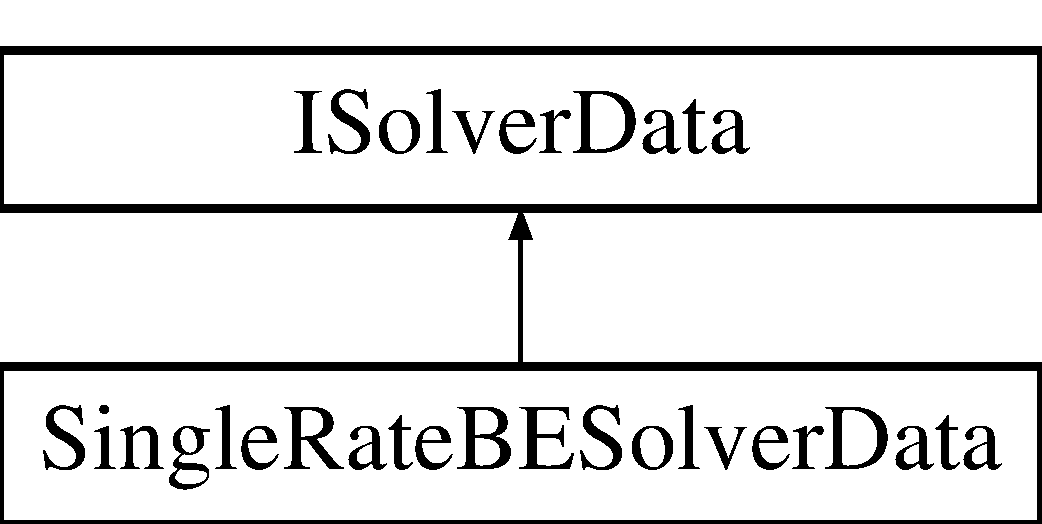
\includegraphics[height=2cm]{classSingleRateBESolverData}
\end{center}
\end{figure}
\subsection*{Public Member Functions}
\begin{DoxyCompactItemize}
\item 
\hypertarget{classSingleRateBESolverData_af7c930c6aa2efb7860957e5044cc3373}{
const RealVector \& {\bfseries getError} () const }
\label{classSingleRateBESolverData_af7c930c6aa2efb7860957e5044cc3373}

\item 
\hypertarget{classSingleRateBESolverData_acb03ac3487e81e10ba857f496da0daaf}{
void {\bfseries setError} (const RealVector \&error)}
\label{classSingleRateBESolverData_acb03ac3487e81e10ba857f496da0daaf}

\item 
\hypertarget{classSingleRateBESolverData_a6db719022becc85e9419c8b6181b200a}{
Real {\bfseries getH} () const }
\label{classSingleRateBESolverData_a6db719022becc85e9419c8b6181b200a}

\item 
\hypertarget{classSingleRateBESolverData_aaef251e585ae5ab4b10b54bfe6076202}{
void {\bfseries setH} (Real h)}
\label{classSingleRateBESolverData_aaef251e585ae5ab4b10b54bfe6076202}

\item 
\hypertarget{classSingleRateBESolverData_a8a7382d33dff89c95be07a32749157d2}{
Bool {\bfseries isHasSucceded} () const }
\label{classSingleRateBESolverData_a8a7382d33dff89c95be07a32749157d2}

\item 
\hypertarget{classSingleRateBESolverData_aee4f7e6c1851c21dda37fae5f5ffb032}{
void {\bfseries setHasSucceded} (Bool hasSucceded)}
\label{classSingleRateBESolverData_aee4f7e6c1851c21dda37fae5f5ffb032}

\item 
\hypertarget{classSingleRateBESolverData_a932176df7eb8fb4a42e99e596555b9cd}{
Real {\bfseries getTime} () const }
\label{classSingleRateBESolverData_a932176df7eb8fb4a42e99e596555b9cd}

\item 
\hypertarget{classSingleRateBESolverData_aabc5e847c66a78c20ef2f464d6c51d75}{
void {\bfseries setTime} (Real time)}
\label{classSingleRateBESolverData_aabc5e847c66a78c20ef2f464d6c51d75}

\item 
\hypertarget{classSingleRateBESolverData_ae210703564ebc8670b0c68ea9e302245}{
const RealVector \& {\bfseries getY} () const }
\label{classSingleRateBESolverData_ae210703564ebc8670b0c68ea9e302245}

\item 
\hypertarget{classSingleRateBESolverData_a1958d758dfd26da3d31efccecd753f1e}{
void {\bfseries setY} (const RealVector \&y)}
\label{classSingleRateBESolverData_a1958d758dfd26da3d31efccecd753f1e}

\item 
\hypertarget{classSingleRateBESolverData_ae86faf1673cc3b31042e2bf363972462}{
const IntegerVector \& {\bfseries getMesh} () const }
\label{classSingleRateBESolverData_ae86faf1673cc3b31042e2bf363972462}

\item 
\hypertarget{classSingleRateBESolverData_aae854bb373d3053328b7913d552af0ac}{
Bool {\bfseries isRefining} () const }
\label{classSingleRateBESolverData_aae854bb373d3053328b7913d552af0ac}

\item 
\hypertarget{classSingleRateBESolverData_a381969dea45142be23a62c1bfccfd300}{
void {\bfseries setRefining} (Bool refining)}
\label{classSingleRateBESolverData_a381969dea45142be23a62c1bfccfd300}

\item 
\hypertarget{classSingleRateBESolverData_a12444469b88c43c5756dfe5039cea6f9}{
const IntegerVector \& {\bfseries getNumbComponentsSolve} () const }
\label{classSingleRateBESolverData_a12444469b88c43c5756dfe5039cea6f9}

\item 
\hypertarget{classSingleRateBESolverData_aa94d2505f9aa0c283d5c4eba73968e76}{
void {\bfseries setNumbComponentsSolve} (const IntegerVector \&numbComponentsSolve)}
\label{classSingleRateBESolverData_aa94d2505f9aa0c283d5c4eba73968e76}

\item 
\hypertarget{classSingleRateBESolverData_ae04c513aea3527d3d70d35c82a333ddd}{
void {\bfseries setMesh} (const IntegerVector \&mesh)}
\label{classSingleRateBESolverData_ae04c513aea3527d3d70d35c82a333ddd}

\end{DoxyCompactItemize}


The documentation for this class was generated from the following files:\begin{DoxyCompactItemize}
\item 
SingleRateBESolver/SingleRateBESolverData.h\item 
SingleRateBESolver/SingleRateBESolverData.cpp\end{DoxyCompactItemize}

\hypertarget{classSingleRateFESolver}{
\section{SingleRateFESolver Class Reference}
\label{classSingleRateFESolver}\index{SingleRateFESolver@{SingleRateFESolver}}
}


Class to define the Singlerate Forward Euler Solver with a fixed time step.  


{\ttfamily \#include $<$SingleRateFESolver.h$>$}Inheritance diagram for SingleRateFESolver::\begin{figure}[H]
\begin{center}
\leavevmode
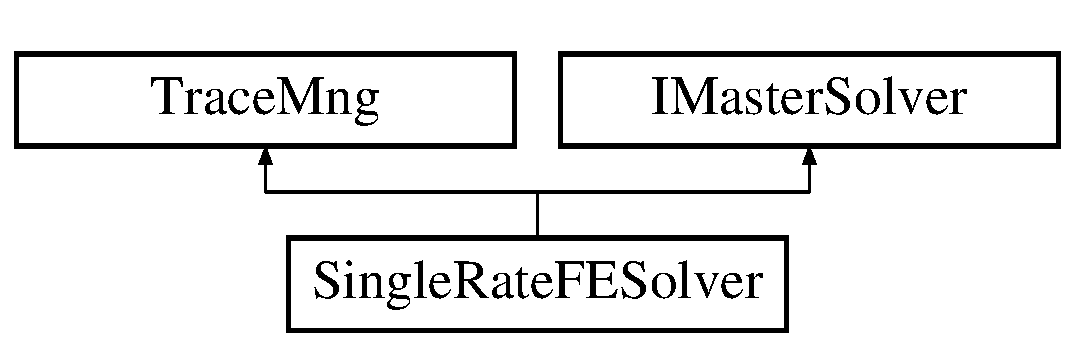
\includegraphics[height=2cm]{classSingleRateFESolver}
\end{center}
\end{figure}
\subsection*{Public Member Functions}
\begin{DoxyCompactItemize}
\item 
\hypertarget{classSingleRateFESolver_a5ea6db6cfefba42530555d2d5c809a08}{
void \hyperlink{classSingleRateFESolver_a5ea6db6cfefba42530555d2d5c809a08}{setFun} (\hyperlink{classIRHSFunction}{IRHSFunction} $\ast$fun)}
\label{classSingleRateFESolver_a5ea6db6cfefba42530555d2d5c809a08}

\begin{DoxyCompactList}\small\item\em Sets the RHS Function. \item\end{DoxyCompactList}\item 
\hypertarget{classSingleRateFESolver_a8db35d4c78e8ee2188bfe5d3c60f8a20}{
void \hyperlink{classSingleRateFESolver_a8db35d4c78e8ee2188bfe5d3c60f8a20}{setNewtSolv} (std::unique\_\-ptr$<$ \hyperlink{classINewtonSolver}{INewtonSolver} $>$ newtSolv)}
\label{classSingleRateFESolver_a8db35d4c78e8ee2188bfe5d3c60f8a20}

\begin{DoxyCompactList}\small\item\em Sets the Newton SOlver. \item\end{DoxyCompactList}\item 
\hypertarget{classSingleRateFESolver_a85f5c7440f89d791f2b5cf31173a591e}{
void \hyperlink{classSingleRateFESolver_a85f5c7440f89d791f2b5cf31173a591e}{setHinitial} (Real hinitial)}
\label{classSingleRateFESolver_a85f5c7440f89d791f2b5cf31173a591e}

\begin{DoxyCompactList}\small\item\em Sets the time step for the first time slab. \item\end{DoxyCompactList}\item 
\hypertarget{classSingleRateFESolver_a0347b664a5941a8d3e2f075c1b42b4bf}{
void \hyperlink{classSingleRateFESolver_a0347b664a5941a8d3e2f075c1b42b4bf}{setHz1initial} (const RealVector \&hz1initial)}
\label{classSingleRateFESolver_a0347b664a5941a8d3e2f075c1b42b4bf}

\begin{DoxyCompactList}\small\item\em Sets the initial guess for the variable z. \item\end{DoxyCompactList}\item 
\hypertarget{classSingleRateFESolver_a1f642b2a50f2ba7a95e418b012b23f1c}{
void \hyperlink{classSingleRateFESolver_a1f642b2a50f2ba7a95e418b012b23f1c}{setTfinal} (Real tfinal)}
\label{classSingleRateFESolver_a1f642b2a50f2ba7a95e418b012b23f1c}

\begin{DoxyCompactList}\small\item\em Sets the final time. \item\end{DoxyCompactList}\item 
\hypertarget{classSingleRateFESolver_a5047dc929dc5a0d68163994999f3bb09}{
void \hyperlink{classSingleRateFESolver_a5047dc929dc5a0d68163994999f3bb09}{setTinitial} (Real tinitial)}
\label{classSingleRateFESolver_a5047dc929dc5a0d68163994999f3bb09}

\begin{DoxyCompactList}\small\item\em Sets the initial time. \item\end{DoxyCompactList}\item 
\hypertarget{classSingleRateFESolver_a07bd5e02b6fcd7c29058f1ab745f2f71}{
void \hyperlink{classSingleRateFESolver_a07bd5e02b6fcd7c29058f1ab745f2f71}{setYinitial} (const RealVector \&yinitial)}
\label{classSingleRateFESolver_a07bd5e02b6fcd7c29058f1ab745f2f71}

\begin{DoxyCompactList}\small\item\em Sets the initial condition. \item\end{DoxyCompactList}\item 
\hypertarget{classSingleRateFESolver_aebb661ca33459dc1bbbecff6f40aeb0a}{
std::vector$<$ std::unique\_\-ptr$<$ \hyperlink{classISolverData}{ISolverData} $>$ $>$ \&\& \hyperlink{classSingleRateFESolver_aebb661ca33459dc1bbbecff6f40aeb0a}{getSolution} ()}
\label{classSingleRateFESolver_aebb661ca33459dc1bbbecff6f40aeb0a}

\begin{DoxyCompactList}\small\item\em Gets the solution vector. \item\end{DoxyCompactList}\item 
\hypertarget{classSingleRateFESolver_aad2d9d77e35451e6e7be6af0162b4623}{
void \hyperlink{classSingleRateFESolver_aad2d9d77e35451e6e7be6af0162b4623}{setNewtonTolAbs} (Real newtonTolAbs)}
\label{classSingleRateFESolver_aad2d9d77e35451e6e7be6af0162b4623}

\begin{DoxyCompactList}\small\item\em Sets the absolute Newton tolerance. \item\end{DoxyCompactList}\item 
\hypertarget{classSingleRateFESolver_a6b84fbec7f7dbf28ba3e42305c60a0a6}{
void \hyperlink{classSingleRateFESolver_a6b84fbec7f7dbf28ba3e42305c60a0a6}{setNewtonTolRel} (Real newtonTolRel)}
\label{classSingleRateFESolver_a6b84fbec7f7dbf28ba3e42305c60a0a6}

\begin{DoxyCompactList}\small\item\em Sets the relative Newton tolerance. \item\end{DoxyCompactList}\item 
\hypertarget{classSingleRateFESolver_ac2b98eed3ec2af8b0708953b2b957031}{
void \hyperlink{classSingleRateFESolver_ac2b98eed3ec2af8b0708953b2b957031}{setErrorTolAbs} (Real errorTolAbs)}
\label{classSingleRateFESolver_ac2b98eed3ec2af8b0708953b2b957031}

\begin{DoxyCompactList}\small\item\em Sets the absolute Error tolerance. \item\end{DoxyCompactList}\item 
\hypertarget{classSingleRateFESolver_a3f93cd51aef89e0ccbdef8b8baf267de}{
void \hyperlink{classSingleRateFESolver_a3f93cd51aef89e0ccbdef8b8baf267de}{setErrorTolRel} (Real errorTolRel)}
\label{classSingleRateFESolver_a3f93cd51aef89e0ccbdef8b8baf267de}

\begin{DoxyCompactList}\small\item\em Sets the relative Error tolerance. \item\end{DoxyCompactList}\item 
void \hyperlink{classSingleRateFESolver_a4beb6ba564a2df02b0c96342646b3be9}{compute} ()
\end{DoxyCompactItemize}


\subsection{Detailed Description}
Class to define the Singlerate Forward Euler Solver with a fixed time step. 

\subsection{Member Function Documentation}
\hypertarget{classSingleRateFESolver_a4beb6ba564a2df02b0c96342646b3be9}{
\index{SingleRateFESolver@{SingleRateFESolver}!compute@{compute}}
\index{compute@{compute}!SingleRateFESolver@{SingleRateFESolver}}
\subsubsection[{compute}]{\setlength{\rightskip}{0pt plus 5cm}void SingleRateFESolver::compute ()\hspace{0.3cm}{\ttfamily  \mbox{[}virtual\mbox{]}}}}
\label{classSingleRateFESolver_a4beb6ba564a2df02b0c96342646b3be9}


First data output: initial conditions

update solution

Store new solution 

Implements \hyperlink{classIMasterSolver}{IMasterSolver}.

The documentation for this class was generated from the following files:\begin{DoxyCompactItemize}
\item 
SingleRateFESolver/SingleRateFESolver.h\item 
SingleRateFESolver/SingleRateFESolver.cpp\end{DoxyCompactItemize}

\hypertarget{classSingleRateFESolverData}{
\section{SingleRateFESolverData Class Reference}
\label{classSingleRateFESolverData}\index{SingleRateFESolverData@{SingleRateFESolverData}}
}
Inheritance diagram for SingleRateFESolverData::\begin{figure}[H]
\begin{center}
\leavevmode
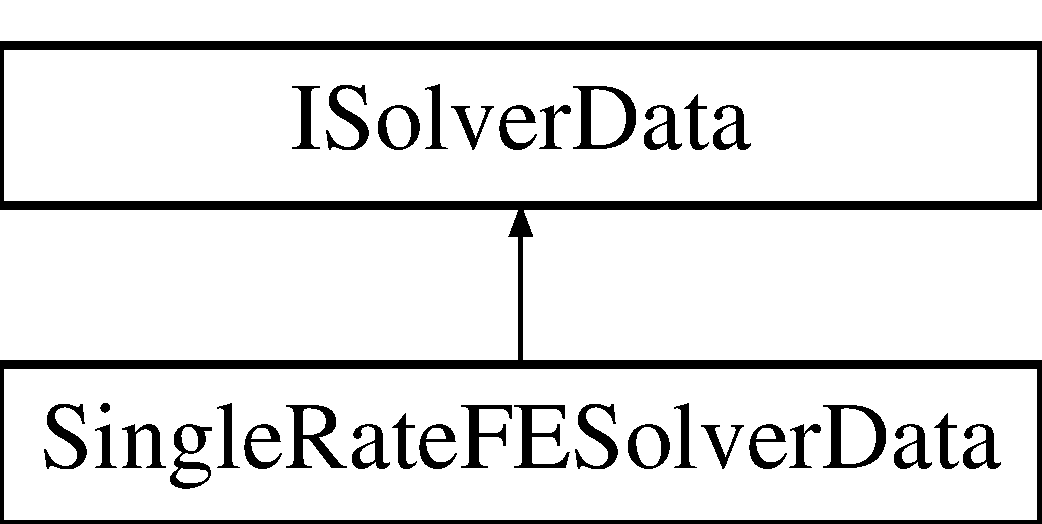
\includegraphics[height=2cm]{classSingleRateFESolverData}
\end{center}
\end{figure}
\subsection*{Public Member Functions}
\begin{DoxyCompactItemize}
\item 
\hypertarget{classSingleRateFESolverData_ac3434371d7fecbe4e03743ce0077cdeb}{
const RealVector \& {\bfseries getError} () const }
\label{classSingleRateFESolverData_ac3434371d7fecbe4e03743ce0077cdeb}

\item 
\hypertarget{classSingleRateFESolverData_a81a42aeacdd1fd83ed0bccef6898ddc2}{
void {\bfseries setError} (const RealVector \&error)}
\label{classSingleRateFESolverData_a81a42aeacdd1fd83ed0bccef6898ddc2}

\item 
\hypertarget{classSingleRateFESolverData_ad6bf6cdcde73d976bb7fa745bc31e354}{
Real {\bfseries getH} () const }
\label{classSingleRateFESolverData_ad6bf6cdcde73d976bb7fa745bc31e354}

\item 
\hypertarget{classSingleRateFESolverData_a29e1329801a0eb8038bb2ffe963760d0}{
void {\bfseries setH} (Real h)}
\label{classSingleRateFESolverData_a29e1329801a0eb8038bb2ffe963760d0}

\item 
\hypertarget{classSingleRateFESolverData_a717b8c79cb9b2c2525b968302f471d3d}{
Bool {\bfseries isHasSucceded} () const }
\label{classSingleRateFESolverData_a717b8c79cb9b2c2525b968302f471d3d}

\item 
\hypertarget{classSingleRateFESolverData_a6f55b5a772d7559f44d30b6ef73ea046}{
void {\bfseries setHasSucceded} (Bool hasSucceded)}
\label{classSingleRateFESolverData_a6f55b5a772d7559f44d30b6ef73ea046}

\item 
\hypertarget{classSingleRateFESolverData_aa0b99b42a8abd1ea09a851e61281157d}{
Real {\bfseries getTime} () const }
\label{classSingleRateFESolverData_aa0b99b42a8abd1ea09a851e61281157d}

\item 
\hypertarget{classSingleRateFESolverData_ac4f7a318943683aab40654d2d5c68d46}{
void {\bfseries setTime} (Real time)}
\label{classSingleRateFESolverData_ac4f7a318943683aab40654d2d5c68d46}

\item 
\hypertarget{classSingleRateFESolverData_a7be74f378da05b81a59b0b2d6983392a}{
const RealVector \& {\bfseries getY} () const }
\label{classSingleRateFESolverData_a7be74f378da05b81a59b0b2d6983392a}

\item 
\hypertarget{classSingleRateFESolverData_a01acff39ea246981730bc410f6ebc78d}{
void {\bfseries setY} (const RealVector \&y)}
\label{classSingleRateFESolverData_a01acff39ea246981730bc410f6ebc78d}

\item 
\hypertarget{classSingleRateFESolverData_a20238df7a7605992c1b88766fd009643}{
const IntegerVector \& {\bfseries getMesh} () const }
\label{classSingleRateFESolverData_a20238df7a7605992c1b88766fd009643}

\item 
\hypertarget{classSingleRateFESolverData_af27ca6658e5f521ed6168d1f7e2a2ca2}{
Bool {\bfseries isRefining} () const }
\label{classSingleRateFESolverData_af27ca6658e5f521ed6168d1f7e2a2ca2}

\item 
\hypertarget{classSingleRateFESolverData_a7b855d3316ff393770edaeb1b313bfd5}{
void {\bfseries setRefining} (Bool refining)}
\label{classSingleRateFESolverData_a7b855d3316ff393770edaeb1b313bfd5}

\item 
\hypertarget{classSingleRateFESolverData_a383c5301131d7a6dad537f9af76fcfb3}{
const IntegerVector \& {\bfseries getNumbComponentsSolve} () const }
\label{classSingleRateFESolverData_a383c5301131d7a6dad537f9af76fcfb3}

\item 
\hypertarget{classSingleRateFESolverData_af51e1c99af7dcdbf7d9f4239d49b27b2}{
void {\bfseries setNumbComponentsSolve} (const IntegerVector \&numbComponentsSolve)}
\label{classSingleRateFESolverData_af51e1c99af7dcdbf7d9f4239d49b27b2}

\item 
\hypertarget{classSingleRateFESolverData_a4ec292a9e1c974ac89452320fbd0663f}{
void {\bfseries setMesh} (const IntegerVector \&mesh)}
\label{classSingleRateFESolverData_a4ec292a9e1c974ac89452320fbd0663f}

\end{DoxyCompactItemize}


The documentation for this class was generated from the following files:\begin{DoxyCompactItemize}
\item 
SingleRateFESolver/SingleRateFESolverData.h\item 
SingleRateFESolver/SingleRateFESolverData.cpp\end{DoxyCompactItemize}

\hypertarget{classSingleRateTRBDF2Solver}{
\section{SingleRateTRBDF2Solver Class Reference}
\label{classSingleRateTRBDF2Solver}\index{SingleRateTRBDF2Solver@{SingleRateTRBDF2Solver}}
}


Class to define the Singlerate TRBDF2 Solver with a fixed time step.  


{\ttfamily \#include $<$SingleRateTRBDF2Solver.h$>$}Inheritance diagram for SingleRateTRBDF2Solver::\begin{figure}[H]
\begin{center}
\leavevmode
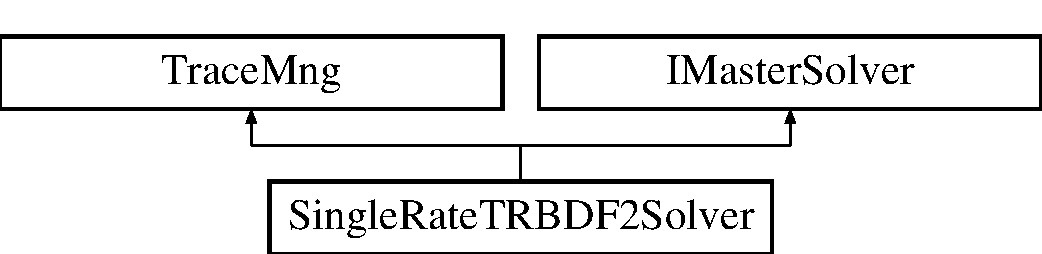
\includegraphics[height=2cm]{classSingleRateTRBDF2Solver}
\end{center}
\end{figure}
\subsection*{Public Member Functions}
\begin{DoxyCompactItemize}
\item 
\hypertarget{classSingleRateTRBDF2Solver_aa9133a77e58a3a4027655cd6de0d5b94}{
void \hyperlink{classSingleRateTRBDF2Solver_aa9133a77e58a3a4027655cd6de0d5b94}{setFun} (\hyperlink{classIRHSFunction}{IRHSFunction} $\ast$fun)}
\label{classSingleRateTRBDF2Solver_aa9133a77e58a3a4027655cd6de0d5b94}

\begin{DoxyCompactList}\small\item\em Sets the RHS Function. \item\end{DoxyCompactList}\item 
\hypertarget{classSingleRateTRBDF2Solver_a5c1f921a270ac422900c127f320e97c9}{
void \hyperlink{classSingleRateTRBDF2Solver_a5c1f921a270ac422900c127f320e97c9}{setNewtSolv} (std::unique\_\-ptr$<$ \hyperlink{classINewtonSolver}{INewtonSolver} $>$ newtSolv)}
\label{classSingleRateTRBDF2Solver_a5c1f921a270ac422900c127f320e97c9}

\begin{DoxyCompactList}\small\item\em Sets the Newton SOlver. \item\end{DoxyCompactList}\item 
\hypertarget{classSingleRateTRBDF2Solver_a1486e389359b8fb68df92c26a73ad0f3}{
void \hyperlink{classSingleRateTRBDF2Solver_a1486e389359b8fb68df92c26a73ad0f3}{setHinitial} (Real hinitial)}
\label{classSingleRateTRBDF2Solver_a1486e389359b8fb68df92c26a73ad0f3}

\begin{DoxyCompactList}\small\item\em Sets the time step for the first time slab. \item\end{DoxyCompactList}\item 
\hypertarget{classSingleRateTRBDF2Solver_a9f33c38922a2b72dfd2d9377ccd5d22a}{
void \hyperlink{classSingleRateTRBDF2Solver_a9f33c38922a2b72dfd2d9377ccd5d22a}{setHz1initial} (const RealVector \&hz1initial)}
\label{classSingleRateTRBDF2Solver_a9f33c38922a2b72dfd2d9377ccd5d22a}

\begin{DoxyCompactList}\small\item\em Sets the initial guess for the variable z. \item\end{DoxyCompactList}\item 
\hypertarget{classSingleRateTRBDF2Solver_a71f0327229d5ea37e769bbf48a6b85d1}{
void \hyperlink{classSingleRateTRBDF2Solver_a71f0327229d5ea37e769bbf48a6b85d1}{setTfinal} (Real tfinal)}
\label{classSingleRateTRBDF2Solver_a71f0327229d5ea37e769bbf48a6b85d1}

\begin{DoxyCompactList}\small\item\em Sets the final time. \item\end{DoxyCompactList}\item 
\hypertarget{classSingleRateTRBDF2Solver_a9f0fa527544f37e8659df2c4c13153d2}{
void \hyperlink{classSingleRateTRBDF2Solver_a9f0fa527544f37e8659df2c4c13153d2}{setTinitial} (Real tinitial)}
\label{classSingleRateTRBDF2Solver_a9f0fa527544f37e8659df2c4c13153d2}

\begin{DoxyCompactList}\small\item\em Sets the initial time. \item\end{DoxyCompactList}\item 
\hypertarget{classSingleRateTRBDF2Solver_a30d1c78ed31b69d7711f3c40a602f78c}{
void \hyperlink{classSingleRateTRBDF2Solver_a30d1c78ed31b69d7711f3c40a602f78c}{setYinitial} (const RealVector \&yinitial)}
\label{classSingleRateTRBDF2Solver_a30d1c78ed31b69d7711f3c40a602f78c}

\begin{DoxyCompactList}\small\item\em Sets the initial condition. \item\end{DoxyCompactList}\item 
\hypertarget{classSingleRateTRBDF2Solver_a406cfcab074805b129bd80006c74843e}{
std::vector$<$ std::unique\_\-ptr$<$ \hyperlink{classISolverData}{ISolverData} $>$ $>$ \&\& \hyperlink{classSingleRateTRBDF2Solver_a406cfcab074805b129bd80006c74843e}{getSolution} ()}
\label{classSingleRateTRBDF2Solver_a406cfcab074805b129bd80006c74843e}

\begin{DoxyCompactList}\small\item\em Gets the solution vector. \item\end{DoxyCompactList}\item 
\hypertarget{classSingleRateTRBDF2Solver_ab221da0f138d4aebe054f4b1fbe91444}{
void \hyperlink{classSingleRateTRBDF2Solver_ab221da0f138d4aebe054f4b1fbe91444}{setNewtonTolAbs} (Real newtonTolAbs)}
\label{classSingleRateTRBDF2Solver_ab221da0f138d4aebe054f4b1fbe91444}

\begin{DoxyCompactList}\small\item\em Sets the absolute Newton tolerance. \item\end{DoxyCompactList}\item 
\hypertarget{classSingleRateTRBDF2Solver_aeb3bfed2c5c7a1b314579b2854f4f64d}{
void \hyperlink{classSingleRateTRBDF2Solver_aeb3bfed2c5c7a1b314579b2854f4f64d}{setNewtonTolRel} (Real newtonTolRel)}
\label{classSingleRateTRBDF2Solver_aeb3bfed2c5c7a1b314579b2854f4f64d}

\begin{DoxyCompactList}\small\item\em Sets the relative Newton tolerance. \item\end{DoxyCompactList}\item 
\hypertarget{classSingleRateTRBDF2Solver_ada3abba75dbb15b4bb524bb7b144f634}{
void \hyperlink{classSingleRateTRBDF2Solver_ada3abba75dbb15b4bb524bb7b144f634}{setErrorTolAbs} (Real errorTolAbs)}
\label{classSingleRateTRBDF2Solver_ada3abba75dbb15b4bb524bb7b144f634}

\begin{DoxyCompactList}\small\item\em Sets the absolute Error tolerance. \item\end{DoxyCompactList}\item 
\hypertarget{classSingleRateTRBDF2Solver_ac951fd8c8caf2292cf9c93a47495b44b}{
void \hyperlink{classSingleRateTRBDF2Solver_ac951fd8c8caf2292cf9c93a47495b44b}{setErrorTolRel} (Real errorTolRel)}
\label{classSingleRateTRBDF2Solver_ac951fd8c8caf2292cf9c93a47495b44b}

\begin{DoxyCompactList}\small\item\em Sets the relative Error tolerance. \item\end{DoxyCompactList}\item 
void \hyperlink{classSingleRateTRBDF2Solver_ab9beae6ea765fe34398a02b7b99da10f}{compute} ()
\end{DoxyCompactItemize}


\subsection{Detailed Description}
Class to define the Singlerate TRBDF2 Solver with a fixed time step. 

\subsection{Member Function Documentation}
\hypertarget{classSingleRateTRBDF2Solver_ab9beae6ea765fe34398a02b7b99da10f}{
\index{SingleRateTRBDF2Solver@{SingleRateTRBDF2Solver}!compute@{compute}}
\index{compute@{compute}!SingleRateTRBDF2Solver@{SingleRateTRBDF2Solver}}
\subsubsection[{compute}]{\setlength{\rightskip}{0pt plus 5cm}void SingleRateTRBDF2Solver::compute ()\hspace{0.3cm}{\ttfamily  \mbox{[}virtual\mbox{]}}}}
\label{classSingleRateTRBDF2Solver_ab9beae6ea765fe34398a02b7b99da10f}


Parameters time step size

First data output: initial conditions

number of consecutive Newton divergence

Calculate the Jacobian and the mixed tolerance

Calculate the solution with TRBDF2 Method

Store the numerical Solution

Newton is OK But some components estimator $>$ Tol

Control restart timestep

Newton is OK But and ALL components estimator $<$ Tol

Propose next timestep

Take into account tfinal bound

Newton divergence 

Implements \hyperlink{classIMasterSolver}{IMasterSolver}.

The documentation for this class was generated from the following files:\begin{DoxyCompactItemize}
\item 
SingleRateTRBDF2Solver/SingleRateTRBDF2Solver.h\item 
SingleRateTRBDF2Solver/SingleRateTRBDF2Solver.cpp\end{DoxyCompactItemize}

\hypertarget{classSingleRateTRBDF2SolverData}{
\section{SingleRateTRBDF2SolverData Class Reference}
\label{classSingleRateTRBDF2SolverData}\index{SingleRateTRBDF2SolverData@{SingleRateTRBDF2SolverData}}
}
Inheritance diagram for SingleRateTRBDF2SolverData::\begin{figure}[H]
\begin{center}
\leavevmode
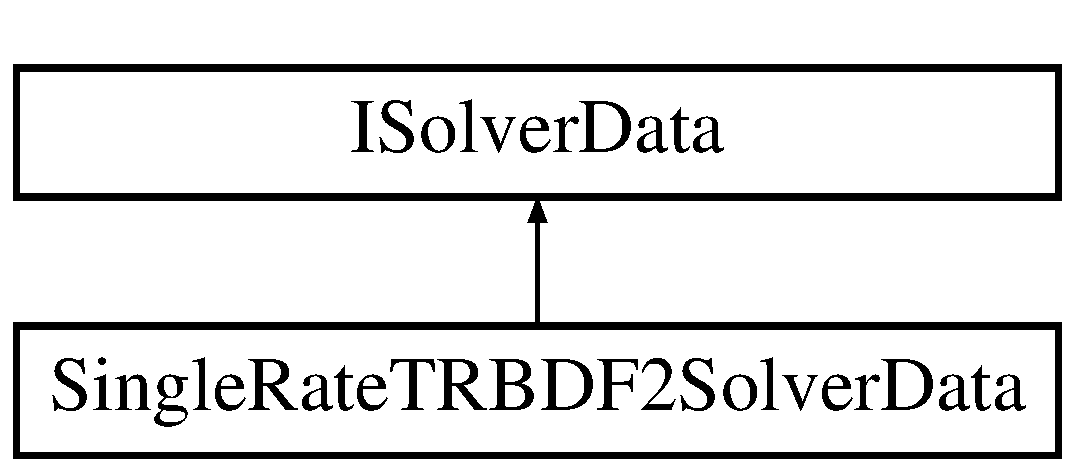
\includegraphics[height=2cm]{classSingleRateTRBDF2SolverData}
\end{center}
\end{figure}
\subsection*{Public Member Functions}
\begin{DoxyCompactItemize}
\item 
\hypertarget{classSingleRateTRBDF2SolverData_a085d2c0a19a46fa12e18819cba60e2af}{
const RealVector \& {\bfseries getError} () const }
\label{classSingleRateTRBDF2SolverData_a085d2c0a19a46fa12e18819cba60e2af}

\item 
\hypertarget{classSingleRateTRBDF2SolverData_a6cfa909f13a7acf3ed3aeb34c5926cb2}{
void {\bfseries setError} (const RealVector \&err)}
\label{classSingleRateTRBDF2SolverData_a6cfa909f13a7acf3ed3aeb34c5926cb2}

\item 
\hypertarget{classSingleRateTRBDF2SolverData_aadaf7a90573d5037133235df9e4f2b27}{
Real {\bfseries getH} () const }
\label{classSingleRateTRBDF2SolverData_aadaf7a90573d5037133235df9e4f2b27}

\item 
\hypertarget{classSingleRateTRBDF2SolverData_a09a791547a21c23934f3b978f0477d1e}{
void {\bfseries setH} (Real vec)}
\label{classSingleRateTRBDF2SolverData_a09a791547a21c23934f3b978f0477d1e}

\item 
\hypertarget{classSingleRateTRBDF2SolverData_a74d19396671b35506a15e1caa0eb6edc}{
Bool {\bfseries isHasSucceded} () const }
\label{classSingleRateTRBDF2SolverData_a74d19396671b35506a15e1caa0eb6edc}

\item 
\hypertarget{classSingleRateTRBDF2SolverData_a938d1fa18a6685c80108876eeedd45b1}{
void {\bfseries setHasSucceded} (Bool hasSucceded)}
\label{classSingleRateTRBDF2SolverData_a938d1fa18a6685c80108876eeedd45b1}

\item 
\hypertarget{classSingleRateTRBDF2SolverData_ad6981cc33ecbe6f1e2c6cc49e490ecbf}{
Real {\bfseries getTime} () const }
\label{classSingleRateTRBDF2SolverData_ad6981cc33ecbe6f1e2c6cc49e490ecbf}

\item 
\hypertarget{classSingleRateTRBDF2SolverData_a76271d91262f664442170ccdd6878999}{
void {\bfseries setTime} (Real t)}
\label{classSingleRateTRBDF2SolverData_a76271d91262f664442170ccdd6878999}

\item 
\hypertarget{classSingleRateTRBDF2SolverData_a8f6cfa06a496b6ef3147004a7178ce04}{
const RealVector \& {\bfseries getY} () const }
\label{classSingleRateTRBDF2SolverData_a8f6cfa06a496b6ef3147004a7178ce04}

\item 
\hypertarget{classSingleRateTRBDF2SolverData_a23f5ac0c1b29ae58e62806022f8bcbbe}{
void {\bfseries setY} (const RealVector \&yn)}
\label{classSingleRateTRBDF2SolverData_a23f5ac0c1b29ae58e62806022f8bcbbe}

\item 
\hypertarget{classSingleRateTRBDF2SolverData_acae22cf473ad1fbc93648b1dfeee8210}{
const IntegerVector \& {\bfseries getMesh} () const }
\label{classSingleRateTRBDF2SolverData_acae22cf473ad1fbc93648b1dfeee8210}

\item 
\hypertarget{classSingleRateTRBDF2SolverData_a8b13e9a4427a55940b331b271f5aa568}{
void {\bfseries setMesh} (const IntegerVector \&mesh)}
\label{classSingleRateTRBDF2SolverData_a8b13e9a4427a55940b331b271f5aa568}

\item 
\hypertarget{classSingleRateTRBDF2SolverData_a7acc7fa4971888b02a68887579eaec72}{
const IntegerVector \& {\bfseries getNumbComponentsSolve} () const }
\label{classSingleRateTRBDF2SolverData_a7acc7fa4971888b02a68887579eaec72}

\item 
\hypertarget{classSingleRateTRBDF2SolverData_a3eb4bd15d699f1e72f3871fa115ba1fc}{
void {\bfseries setNumbComponentsSolve} (const IntegerVector \&numbComponentsSolve)}
\label{classSingleRateTRBDF2SolverData_a3eb4bd15d699f1e72f3871fa115ba1fc}

\item 
\hypertarget{classSingleRateTRBDF2SolverData_adb6bf2a597a12c7759f51f810bc2b401}{
Bool {\bfseries isRefining} () const }
\label{classSingleRateTRBDF2SolverData_adb6bf2a597a12c7759f51f810bc2b401}

\item 
\hypertarget{classSingleRateTRBDF2SolverData_ac11077f8a3c4021d6d80d1b691304797}{
void {\bfseries setRefining} (Bool refining)}
\label{classSingleRateTRBDF2SolverData_ac11077f8a3c4021d6d80d1b691304797}

\end{DoxyCompactItemize}


The documentation for this class was generated from the following files:\begin{DoxyCompactItemize}
\item 
SingleRateTRBDF2Solver/SingleRateTRBDF2SolverData.h\item 
SingleRateTRBDF2Solver/SingleRateTRBDF2SolverData.cpp\end{DoxyCompactItemize}

\hypertarget{classTraceMng}{
\section{TraceMng Class Reference}
\label{classTraceMng}\index{TraceMng@{TraceMng}}
}
Inheritance diagram for TraceMng::\begin{figure}[H]
\begin{center}
\leavevmode
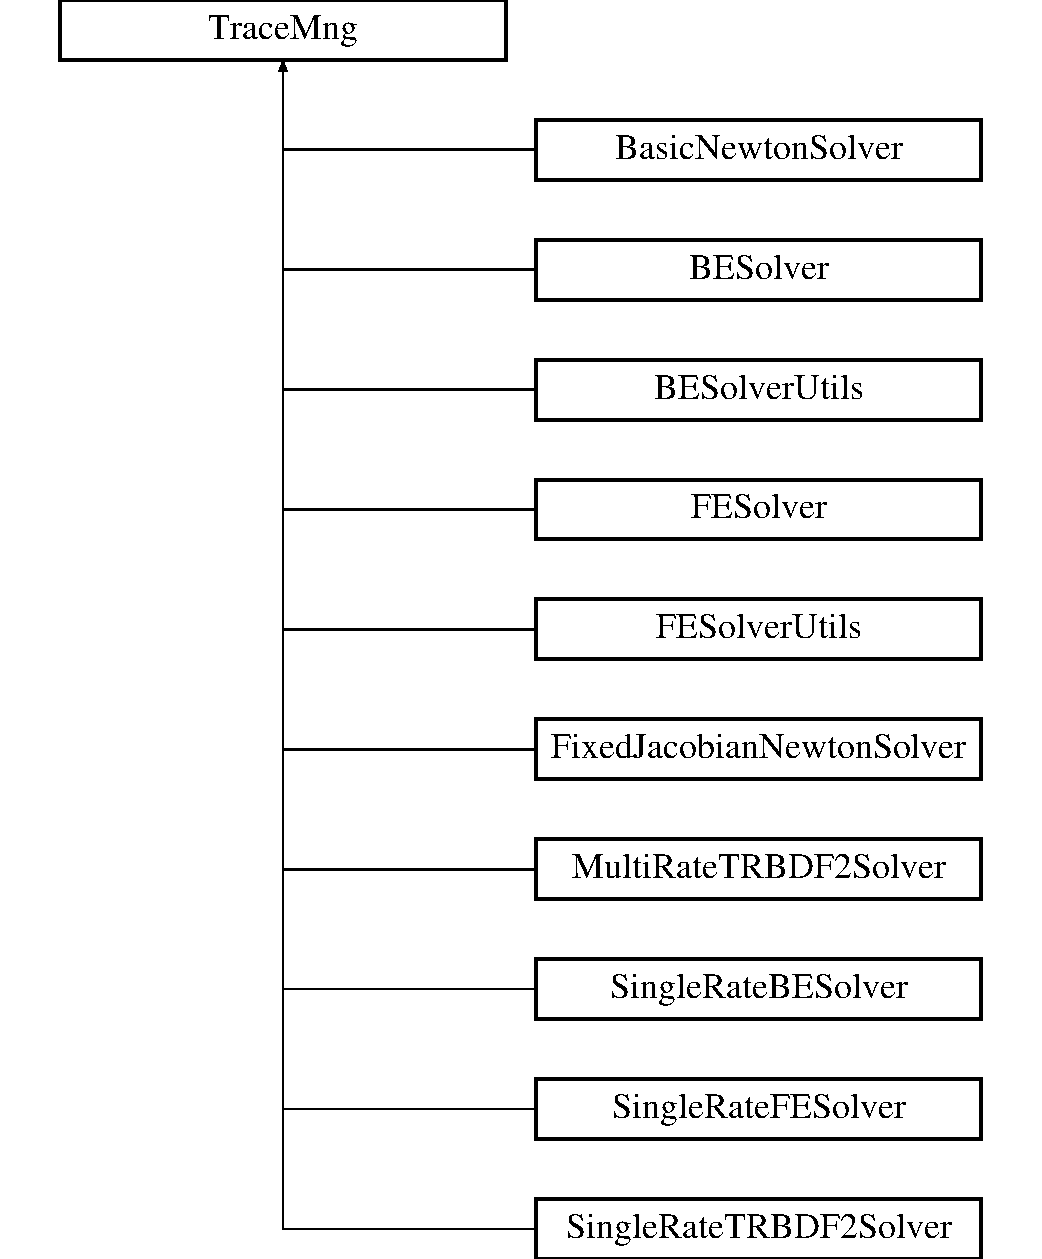
\includegraphics[height=11cm]{classTraceMng}
\end{center}
\end{figure}
\subsection*{Public Member Functions}
\begin{DoxyCompactItemize}
\item 
\hypertarget{classTraceMng_a97874ba8114182fe38e7bbe4a7c8d847}{
void {\bfseries setIsInfo} (bool is\_\-info)}
\label{classTraceMng_a97874ba8114182fe38e7bbe4a7c8d847}

\item 
\hypertarget{classTraceMng_abc1600f6aa416e4e0fc0a9bb8c5fb83d}{
void {\bfseries setIsDebug} (bool is\_\-debug)}
\label{classTraceMng_abc1600f6aa416e4e0fc0a9bb8c5fb83d}

\item 
\hypertarget{classTraceMng_a1bd397263da82f212a67033973bdbde2}{
\hyperlink{classTraceOut}{TraceOut} \& {\bfseries info} ()}
\label{classTraceMng_a1bd397263da82f212a67033973bdbde2}

\item 
\hypertarget{classTraceMng_ac0567336aae4223773ebe5328c916705}{
\hyperlink{classTraceOut}{TraceOut} \& {\bfseries debug} ()}
\label{classTraceMng_ac0567336aae4223773ebe5328c916705}

\item 
\hypertarget{classTraceMng_ad740a852e77265588f6c24733fcb6ca4}{
\hyperlink{classTraceOut}{TraceOut} \& {\bfseries fatal} ()}
\label{classTraceMng_ad740a852e77265588f6c24733fcb6ca4}

\end{DoxyCompactItemize}


The documentation for this class was generated from the following file:\begin{DoxyCompactItemize}
\item 
TraceMng.h\end{DoxyCompactItemize}

\hypertarget{classTraceOut}{
\section{TraceOut Class Reference}
\label{classTraceOut}\index{TraceOut@{TraceOut}}
}
\subsection*{Classes}
\begin{DoxyCompactItemize}
\item 
class \hyperlink{classTraceOut_1_1Flux}{Flux}
\end{DoxyCompactItemize}
\subsection*{Public Member Functions}
\begin{DoxyCompactItemize}
\item 
\hypertarget{classTraceOut_a6fc2da1f125f092d961ec4144ea158af}{
{\bfseries TraceOut} (std::ostream \&os=std::cout)}
\label{classTraceOut_a6fc2da1f125f092d961ec4144ea158af}

\item 
\hypertarget{classTraceOut_aa6249f0fc83fa27c5b7becb8018ba6d3}{
void {\bfseries setIsFatal} (bool is\_\-fatal)}
\label{classTraceOut_aa6249f0fc83fa27c5b7becb8018ba6d3}

\item 
\hypertarget{classTraceOut_a3ca1a57d2cb8dacc4d0ba720063d47cd}{
void {\bfseries setTag} (std::string tag)}
\label{classTraceOut_a3ca1a57d2cb8dacc4d0ba720063d47cd}

\item 
\hypertarget{classTraceOut_a91e06f67c42be20d6951bb1e5df97516}{
void {\bfseries insertTag} ()}
\label{classTraceOut_a91e06f67c42be20d6951bb1e5df97516}

\end{DoxyCompactItemize}
\subsection*{Public Attributes}
\begin{DoxyCompactItemize}
\item 
\hypertarget{classTraceOut_adcb025b62f5f29506eddf2499b3cbee3}{
std::ostream \& {\bfseries m\_\-os}}
\label{classTraceOut_adcb025b62f5f29506eddf2499b3cbee3}

\item 
\hypertarget{classTraceOut_a554933716accee192ba86bd9241467f8}{
bool {\bfseries m\_\-is\_\-fatal}}
\label{classTraceOut_a554933716accee192ba86bd9241467f8}

\end{DoxyCompactItemize}


The documentation for this class was generated from the following file:\begin{DoxyCompactItemize}
\item 
TraceMng.h\end{DoxyCompactItemize}

\hypertarget{classTRBDF2Solver}{
\section{TRBDF2Solver Class Reference}
\label{classTRBDF2Solver}\index{TRBDF2Solver@{TRBDF2Solver}}
}
\subsection*{Public Member Functions}
\begin{DoxyCompactItemize}
\item 
\hypertarget{classTRBDF2Solver_a0e317994696c267ea08324e1d7041c59}{
void {\bfseries setInput} (const \hyperlink{classTRBDF2SolverInput}{TRBDF2SolverInput} \&input)}
\label{classTRBDF2Solver_a0e317994696c267ea08324e1d7041c59}

\item 
\hypertarget{classTRBDF2Solver_a8c4b2abc5cdbff58ca9286e7ba899e38}{
const \hyperlink{classTRBDF2SolverOutput}{TRBDF2SolverOutput} \& {\bfseries getOutput} () const }
\label{classTRBDF2Solver_a8c4b2abc5cdbff58ca9286e7ba899e38}

\item 
\hypertarget{classTRBDF2Solver_a37b7ddb1a13f344665990ed84b3efd9e}{
void {\bfseries setOutput} (const \hyperlink{classTRBDF2SolverOutput}{TRBDF2SolverOutput} \&output)}
\label{classTRBDF2Solver_a37b7ddb1a13f344665990ed84b3efd9e}

\item 
\hypertarget{classTRBDF2Solver_a4d482b9450e446cda5491e394aa61b8a}{
void {\bfseries setRhsFun} (\hyperlink{classIRHSFunction}{IRHSFunction} $\ast$rhsFun)}
\label{classTRBDF2Solver_a4d482b9450e446cda5491e394aa61b8a}

\item 
\hypertarget{classTRBDF2Solver_a085c0f2134957bca52d7d0ca60eedf68}{
void {\bfseries setNewtSolv} (std::unique\_\-ptr$<$ \hyperlink{classINewtonSolver}{INewtonSolver} $>$ newtSolv)}
\label{classTRBDF2Solver_a085c0f2134957bca52d7d0ca60eedf68}

\item 
void \hyperlink{classTRBDF2Solver_a852ad825d56d976c1654135a8eb449a1}{compute} ()
\item 
\hypertarget{classTRBDF2Solver_a920ec7e4bfbc6f356254c41e82fe11be}{
const \hyperlink{classTRBDF2SolverParameters}{TRBDF2SolverParameters} \& {\bfseries getParam} () const }
\label{classTRBDF2Solver_a920ec7e4bfbc6f356254c41e82fe11be}

\item 
\hypertarget{classTRBDF2Solver_a3ede6ffaa21cc65f1e641a5ef7e540f8}{
void {\bfseries setParam} (\hyperlink{classTRBDF2SolverParameters}{TRBDF2SolverParameters} \&param)}
\label{classTRBDF2Solver_a3ede6ffaa21cc65f1e641a5ef7e540f8}

\end{DoxyCompactItemize}


\subsection{Member Function Documentation}
\hypertarget{classTRBDF2Solver_a852ad825d56d976c1654135a8eb449a1}{
\index{TRBDF2Solver@{TRBDF2Solver}!compute@{compute}}
\index{compute@{compute}!TRBDF2Solver@{TRBDF2Solver}}
\subsubsection[{compute}]{\setlength{\rightskip}{0pt plus 5cm}void TRBDF2Solver::compute ()}}
\label{classTRBDF2Solver_a852ad825d56d976c1654135a8eb449a1}


Store the input values

Store the parameters that are necessary for TRBDF2 method

We split the code in two cases: the case that we have to compute the solution for all the components, the case where we have to compute the solution only for some components.

We compute the solution for all the components

Set the Newton function for the z variables and not for y z variables represent $ z(x,t) = h y'(x,t) $ where h is the time step.

We compute the solution for some components 

The documentation for this class was generated from the following files:\begin{DoxyCompactItemize}
\item 
TRBDF2Solver/TRBDF2Solver.h\item 
TRBDF2Solver/TRBDF2Solver.cpp\end{DoxyCompactItemize}

\hypertarget{classTRBDF2SolverInput}{
\section{TRBDF2SolverInput Class Reference}
\label{classTRBDF2SolverInput}\index{TRBDF2SolverInput@{TRBDF2SolverInput}}
}
\subsection*{Public Member Functions}
\begin{DoxyCompactItemize}
\item 
\hypertarget{classTRBDF2SolverInput_a9fd420dd043b684b0f011d9af2df03b5}{
void {\bfseries setInput} (Real t0, Real h, RealVector \&hz1, RealVector \&y0, RealVector \&y1, RealVector \&y2, RealMatrixSparse \&matrixiter, Real tolAbsolute, Real tolRelative, IntegerVector \&ref)}
\label{classTRBDF2SolverInput_a9fd420dd043b684b0f011d9af2df03b5}

\item 
\hypertarget{classTRBDF2SolverInput_ad17ef1264c9b34eb90c4e198cb732a66}{
Real {\bfseries getH} () const }
\label{classTRBDF2SolverInput_ad17ef1264c9b34eb90c4e198cb732a66}

\item 
\hypertarget{classTRBDF2SolverInput_a3c900fc6d938eb96f503f320cf653d04}{
RealVector \& {\bfseries getHz1} ()}
\label{classTRBDF2SolverInput_a3c900fc6d938eb96f503f320cf653d04}

\item 
\hypertarget{classTRBDF2SolverInput_aab9af0524f1c8c9ec1cfb9460f2eddb4}{
Real {\bfseries getT0} () const }
\label{classTRBDF2SolverInput_aab9af0524f1c8c9ec1cfb9460f2eddb4}

\item 
\hypertarget{classTRBDF2SolverInput_abd3aa47d16618f0aa93534ea135c2880}{
Real {\bfseries getTolAbs} () const }
\label{classTRBDF2SolverInput_abd3aa47d16618f0aa93534ea135c2880}

\item 
\hypertarget{classTRBDF2SolverInput_a214a679ef02dd617899af1268490def8}{
Real {\bfseries getTolRel} () const }
\label{classTRBDF2SolverInput_a214a679ef02dd617899af1268490def8}

\item 
\hypertarget{classTRBDF2SolverInput_a410a22478989c4810d8e584beff01dba}{
RealVector \& {\bfseries getY0} ()}
\label{classTRBDF2SolverInput_a410a22478989c4810d8e584beff01dba}

\item 
\hypertarget{classTRBDF2SolverInput_a55c49a8db7dd1ee1e44c62b04d856e83}{
RealMatrixSparse \& {\bfseries getMatrixIter} ()}
\label{classTRBDF2SolverInput_a55c49a8db7dd1ee1e44c62b04d856e83}

\item 
\hypertarget{classTRBDF2SolverInput_a41aa3e4674a8a7aa12f707bbc68794c3}{
const IntegerVector \& {\bfseries getRef} () const }
\label{classTRBDF2SolverInput_a41aa3e4674a8a7aa12f707bbc68794c3}

\item 
\hypertarget{classTRBDF2SolverInput_a9ffded951fea08aed619a88429c7c516}{
const RealVector \& {\bfseries getY1} () const }
\label{classTRBDF2SolverInput_a9ffded951fea08aed619a88429c7c516}

\item 
\hypertarget{classTRBDF2SolverInput_a0812b9c8263ff2e8614749188d9ec7fc}{
const RealVector \& {\bfseries getY2} () const }
\label{classTRBDF2SolverInput_a0812b9c8263ff2e8614749188d9ec7fc}

\end{DoxyCompactItemize}


The documentation for this class was generated from the following files:\begin{DoxyCompactItemize}
\item 
TRBDF2Solver/TRBDF2SolverInput.h\item 
TRBDF2Solver/TRBDF2SolverInput.cpp\end{DoxyCompactItemize}

\hypertarget{classTRBDF2SolverNewtonFunction}{
\section{TRBDF2SolverNewtonFunction Class Reference}
\label{classTRBDF2SolverNewtonFunction}\index{TRBDF2SolverNewtonFunction@{TRBDF2SolverNewtonFunction}}
}
Inheritance diagram for TRBDF2SolverNewtonFunction::\begin{figure}[H]
\begin{center}
\leavevmode
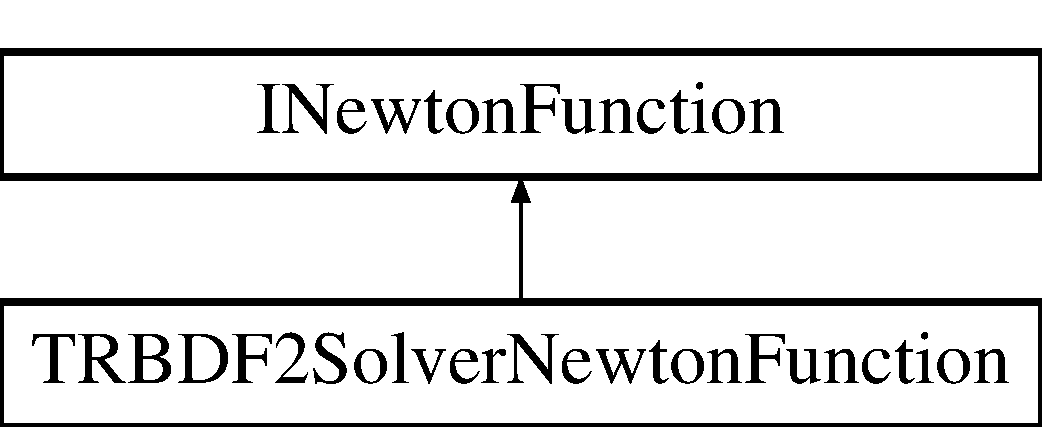
\includegraphics[height=2cm]{classTRBDF2SolverNewtonFunction}
\end{center}
\end{figure}
\subsection*{Public Member Functions}
\begin{DoxyCompactItemize}
\item 
\hypertarget{classTRBDF2SolverNewtonFunction_a6ac29ab69be7c879fc2a271367fbcf07}{
void {\bfseries setDt} (Real dt)}
\label{classTRBDF2SolverNewtonFunction_a6ac29ab69be7c879fc2a271367fbcf07}

\item 
\hypertarget{classTRBDF2SolverNewtonFunction_a1daccfe7b6c0294a4601f3995f7af41d}{
void {\bfseries setFun} (\hyperlink{classIRHSFunction}{IRHSFunction} $\ast$fun)}
\label{classTRBDF2SolverNewtonFunction_a1daccfe7b6c0294a4601f3995f7af41d}

\item 
\hypertarget{classTRBDF2SolverNewtonFunction_a87a2b42923fa544d55a3673ae14dc726}{
void {\bfseries setYn} (RealVector \&ya)}
\label{classTRBDF2SolverNewtonFunction_a87a2b42923fa544d55a3673ae14dc726}

\item 
\hypertarget{classTRBDF2SolverNewtonFunction_a29af111aaa1e51f6bb2180561f970f8f}{
void {\bfseries setTnp} (Real tnp)}
\label{classTRBDF2SolverNewtonFunction_a29af111aaa1e51f6bb2180561f970f8f}

\item 
\hypertarget{classTRBDF2SolverNewtonFunction_a89793efd91dbd70e0a0e475f6d1c1be4}{
void {\bfseries setRef} (IntegerVector \&ref)}
\label{classTRBDF2SolverNewtonFunction_a89793efd91dbd70e0a0e475f6d1c1be4}

\item 
\hypertarget{classTRBDF2SolverNewtonFunction_a7203850686dcc6cd5d9d73822eb53c8a}{
void {\bfseries setD} (Real d)}
\label{classTRBDF2SolverNewtonFunction_a7203850686dcc6cd5d9d73822eb53c8a}

\item 
\hypertarget{classTRBDF2SolverNewtonFunction_a94cb1f31efc579ee0a60f5a6b42bb38e}{
void \hyperlink{classTRBDF2SolverNewtonFunction_a94cb1f31efc579ee0a60f5a6b42bb38e}{evalFJ} (RealVector \&Y, RealVector \&F, RealMatrixSparse \&J)}
\label{classTRBDF2SolverNewtonFunction_a94cb1f31efc579ee0a60f5a6b42bb38e}

\begin{DoxyCompactList}\small\item\em Returns as references the evaluate of Newton function (F) and Newton Jacobian (J) for the vector Y. \item\end{DoxyCompactList}\item 
\hypertarget{classTRBDF2SolverNewtonFunction_aabc2c4aa7517049cec92ce9819f6ce18}{
void \hyperlink{classTRBDF2SolverNewtonFunction_aabc2c4aa7517049cec92ce9819f6ce18}{evalF} (RealVector \&Y, RealVector \&F)}
\label{classTRBDF2SolverNewtonFunction_aabc2c4aa7517049cec92ce9819f6ce18}

\begin{DoxyCompactList}\small\item\em Returns as reference the evaluate of Newton function (F) for the vector Y. \item\end{DoxyCompactList}\end{DoxyCompactItemize}


The documentation for this class was generated from the following files:\begin{DoxyCompactItemize}
\item 
TRBDF2SolverNewtonFunction/TRBDF2SolverNewtonFunction.h\item 
TRBDF2SolverNewtonFunction/TRBDF2SolverNewtonFunction.cpp\end{DoxyCompactItemize}

\hypertarget{classTRBDF2SolverOutput}{
\section{TRBDF2SolverOutput Class Reference}
\label{classTRBDF2SolverOutput}\index{TRBDF2SolverOutput@{TRBDF2SolverOutput}}
}
\subsection*{Public Member Functions}
\begin{DoxyCompactItemize}
\item 
\hypertarget{classTRBDF2SolverOutput_ada9dea9ffe820a17b734a87461b91d4d}{
const RealVector \& {\bfseries getEst} () const }
\label{classTRBDF2SolverOutput_ada9dea9ffe820a17b734a87461b91d4d}

\item 
\hypertarget{classTRBDF2SolverOutput_af2f93169a340a6ab4a8a99b8d71c8a6c}{
void {\bfseries setEst} (const RealVector \&est)}
\label{classTRBDF2SolverOutput_af2f93169a340a6ab4a8a99b8d71c8a6c}

\item 
\hypertarget{classTRBDF2SolverOutput_a665a9fed4e9a09040f241a9f6f4a0e8d}{
Bool {\bfseries isNewtonDiverge} () const }
\label{classTRBDF2SolverOutput_a665a9fed4e9a09040f241a9f6f4a0e8d}

\item 
\hypertarget{classTRBDF2SolverOutput_a79f99dd83f2a1b46a802524efb07bea6}{
void {\bfseries setNewtonDiverge} (Bool newtonDiverge)}
\label{classTRBDF2SolverOutput_a79f99dd83f2a1b46a802524efb07bea6}

\item 
\hypertarget{classTRBDF2SolverOutput_a69b37f83acdcd8428b9ca8da2371ca9e}{
Real {\bfseries getT2} () const }
\label{classTRBDF2SolverOutput_a69b37f83acdcd8428b9ca8da2371ca9e}

\item 
\hypertarget{classTRBDF2SolverOutput_aa1786344740daff82d03595d328fa65a}{
void {\bfseries setT2} (Real t2)}
\label{classTRBDF2SolverOutput_aa1786344740daff82d03595d328fa65a}

\item 
\hypertarget{classTRBDF2SolverOutput_ac337515f4fa142662c1c1b05c7e9f60b}{
const RealVector \& {\bfseries getY2} () const }
\label{classTRBDF2SolverOutput_ac337515f4fa142662c1c1b05c7e9f60b}

\item 
\hypertarget{classTRBDF2SolverOutput_a67f38e014fe4d677cba7091e4e440d49}{
void {\bfseries setY2} (const RealVector \&y2)}
\label{classTRBDF2SolverOutput_a67f38e014fe4d677cba7091e4e440d49}

\item 
\hypertarget{classTRBDF2SolverOutput_aa0ed760c1abf0c0d84a301c7ca207533}{
const RealVector \& {\bfseries getZ2} () const }
\label{classTRBDF2SolverOutput_aa0ed760c1abf0c0d84a301c7ca207533}

\item 
\hypertarget{classTRBDF2SolverOutput_a6b5c18bc78394e18372723a87f4bb134}{
void {\bfseries setZ2} (const RealVector \&z2)}
\label{classTRBDF2SolverOutput_a6b5c18bc78394e18372723a87f4bb134}

\item 
\hypertarget{classTRBDF2SolverOutput_af17ecb422f1b60fa63c7acbb2249bb1c}{
Real {\bfseries getT1} () const }
\label{classTRBDF2SolverOutput_af17ecb422f1b60fa63c7acbb2249bb1c}

\item 
\hypertarget{classTRBDF2SolverOutput_a58cee4a42fe8c8363a4cc442b236edbf}{
void {\bfseries setT1} (Real t1)}
\label{classTRBDF2SolverOutput_a58cee4a42fe8c8363a4cc442b236edbf}

\item 
\hypertarget{classTRBDF2SolverOutput_a9a9241061b20569c65d90599a9bbaaaf}{
const RealVector \& {\bfseries getY1} () const }
\label{classTRBDF2SolverOutput_a9a9241061b20569c65d90599a9bbaaaf}

\item 
\hypertarget{classTRBDF2SolverOutput_a1c72f8f41f4be088a9ee59aa04a3487a}{
void {\bfseries setY1} (const RealVector \&y1)}
\label{classTRBDF2SolverOutput_a1c72f8f41f4be088a9ee59aa04a3487a}

\item 
\hypertarget{classTRBDF2SolverOutput_a7c0a761d421ed91c77ae9353c21efd44}{
const RealVector \& {\bfseries getZ0} () const }
\label{classTRBDF2SolverOutput_a7c0a761d421ed91c77ae9353c21efd44}

\item 
\hypertarget{classTRBDF2SolverOutput_a0d60332dafe04aeb309c6d3f4b19d6f2}{
void {\bfseries setZ0} (const RealVector \&z0)}
\label{classTRBDF2SolverOutput_a0d60332dafe04aeb309c6d3f4b19d6f2}

\item 
\hypertarget{classTRBDF2SolverOutput_a25eddadb39872f554829aa4d766a150e}{
const RealVector \& {\bfseries getZ1} () const }
\label{classTRBDF2SolverOutput_a25eddadb39872f554829aa4d766a150e}

\item 
\hypertarget{classTRBDF2SolverOutput_a9297774be02296f8df5fa3cd51026405}{
void {\bfseries setZ1} (const RealVector \&z1)}
\label{classTRBDF2SolverOutput_a9297774be02296f8df5fa3cd51026405}

\end{DoxyCompactItemize}


The documentation for this class was generated from the following files:\begin{DoxyCompactItemize}
\item 
TRBDF2Solver/TRBDF2SolverOutput.h\item 
TRBDF2Solver/TRBDF2SolverOutput.cpp\end{DoxyCompactItemize}

\hypertarget{classTRBDF2SolverParameters}{
\section{TRBDF2SolverParameters Class Reference}
\label{classTRBDF2SolverParameters}\index{TRBDF2SolverParameters@{TRBDF2SolverParameters}}
}
\subsection*{Public Member Functions}
\begin{DoxyCompactItemize}
\item 
\hypertarget{classTRBDF2SolverParameters_a6b8d26128e0d81ea1e2b1f8139744855}{
Real {\bfseries getD} () const }
\label{classTRBDF2SolverParameters_a6b8d26128e0d81ea1e2b1f8139744855}

\item 
\hypertarget{classTRBDF2SolverParameters_adc7b9fde1606291972f216093b436990}{
Real {\bfseries getE0} () const }
\label{classTRBDF2SolverParameters_adc7b9fde1606291972f216093b436990}

\item 
\hypertarget{classTRBDF2SolverParameters_abd9d6dcce2e1c788a6f24f98df3f438a}{
Real {\bfseries getE1} () const }
\label{classTRBDF2SolverParameters_abd9d6dcce2e1c788a6f24f98df3f438a}

\item 
\hypertarget{classTRBDF2SolverParameters_ab1d976394715dff2a66ae23404a465bf}{
Real {\bfseries getE2} () const }
\label{classTRBDF2SolverParameters_ab1d976394715dff2a66ae23404a465bf}

\item 
\hypertarget{classTRBDF2SolverParameters_a3e4bfd6d63d25c83656955185752186d}{
Real {\bfseries getGm} () const }
\label{classTRBDF2SolverParameters_a3e4bfd6d63d25c83656955185752186d}

\item 
\hypertarget{classTRBDF2SolverParameters_a7e3e230c6a5aa1a0c54e61ce8d6084bc}{
Real {\bfseries getPd0} () const }
\label{classTRBDF2SolverParameters_a7e3e230c6a5aa1a0c54e61ce8d6084bc}

\item 
\hypertarget{classTRBDF2SolverParameters_a99e4fc0ed2b76c38fe59e26261cf7f8a}{
Real {\bfseries getPd1} () const }
\label{classTRBDF2SolverParameters_a99e4fc0ed2b76c38fe59e26261cf7f8a}

\item 
\hypertarget{classTRBDF2SolverParameters_ada5e8684bb05b56ccecc61aceb85c4b8}{
Real {\bfseries getPd2} () const }
\label{classTRBDF2SolverParameters_ada5e8684bb05b56ccecc61aceb85c4b8}

\item 
\hypertarget{classTRBDF2SolverParameters_ae1d53917ac10e1b0472a6c5b057c9b32}{
Real {\bfseries getW} () const }
\label{classTRBDF2SolverParameters_ae1d53917ac10e1b0472a6c5b057c9b32}

\item 
\hypertarget{classTRBDF2SolverParameters_a3420dd67088ff3f7074e0920449d128c}{
void {\bfseries setParam} (Real pd0, Real pd1, Real pd2, Real e0, Real e1, Real e2, Real gm, Real d, Real w)}
\label{classTRBDF2SolverParameters_a3420dd67088ff3f7074e0920449d128c}

\end{DoxyCompactItemize}


The documentation for this class was generated from the following files:\begin{DoxyCompactItemize}
\item 
TRBDF2Solver/TRBDF2SolverParameters.h\item 
TRBDF2Solver/TRBDF2SolverParameters.cpp\end{DoxyCompactItemize}

\hypertarget{classRestab_1_1VariableDescription}{
\section{Restab::VariableDescription Class Reference}
\label{classRestab_1_1VariableDescription}\index{Restab::VariableDescription@{Restab::VariableDescription}}
}
\subsection*{Public Member Functions}
\begin{DoxyCompactItemize}
\item 
\hypertarget{classRestab_1_1VariableDescription_a6795aa78bc476d2365306b541bce638d}{
{\bfseries VariableDescription} (String \_\-label)}
\label{classRestab_1_1VariableDescription_a6795aa78bc476d2365306b541bce638d}

\end{DoxyCompactItemize}
\subsection*{Public Attributes}
\begin{DoxyCompactItemize}
\item 
\hypertarget{classRestab_1_1VariableDescription_a301681d4330fd51074568bb388af72e2}{
String {\bfseries label}}
\label{classRestab_1_1VariableDescription_a301681d4330fd51074568bb388af72e2}

\end{DoxyCompactItemize}


The documentation for this class was generated from the following file:\begin{DoxyCompactItemize}
\item 
Restab.h\end{DoxyCompactItemize}

\hypertarget{classstd_1_1vector}{
\section{vector Class Reference}
\label{classstd_1_1vector}\index{std::vector@{std::vector}}
}


Inherited by \hyperlink{classRestab_1_1Array}{Restab::Array$<$ IndexDescription $>$}, \hyperlink{classRestab_1_1Array}{Restab::Array$<$ MapInteger $>$}, \hyperlink{classRestab_1_1Array}{Restab::Array$<$ MapReal $>$}, and \hyperlink{classRestab_1_1Array}{Restab::Array$<$ VariableDescription $>$}.

The documentation for this class was generated from the following file:\begin{DoxyCompactItemize}
\item 
Restab.h\end{DoxyCompactItemize}

\printindex
\end{document}
